\documentclass{article}

\usepackage{setspace}
\usepackage{float}
\usepackage{apacite}
\usepackage{lipsum}
\usepackage{graphicx}
\usepackage{amsmath}
\usepackage{kbordermatrix}
\usepackage{mathrsfs}
\usepackage{subcaption}
\usepackage{multirow}
\usepackage{siunitx}
\usepackage{pbox}
\usepackage [autostyle, english = american]{csquotes}
%\usepackage{draftwatermark}
\usepackage{booktabs}% http://ctan.org/pkg/booktabs
\usepackage[hyphens,spaces,obeyspaces]{url}

\newcommand{\tabitem}{~~\llap{\textbullet}~~}
%\SetWatermarkText{Draft-5}
%\SetWatermarkScale{1}
\MakeOuterQuote{"}
\hyphenation{Bay-es-ian
             data-base
             data-bases
             Sw-ain}
\newenvironment{conditions}
  {\par\vspace{\abovedisplayskip}\noindent\begin{tabular}{>{$}l<{$} @{${}={}$} l}}
  {\end{tabular}\par\vspace{\belowdisplayskip}}
\captionsetup{font=doublespacing}% Double-spaced float captions

\doublespacing% Double-spaced document text


\title{
\textsc{Reactor Design - Literature review}\\[2.6cm]
{\LARGE \bfseries Nuclear Power for Space Propulsion Systems}\\{\Large\bfseries Mission to the Oort cloud}
}

\author{
D. Fish 
\and 
S. Kerber
\and
R. France
\and
G. L'Her
}

\date{
\textsc{Supervisor:} Jeffrey King\\[1em]
\today
}

\begin{document}

\maketitle
\newpage

\singlespacing
\tableofcontents
\newpage
\listoffigures
\newpage
\doublespacing

%\begin{abstract}%   %NOTE: Deleting the percentage after "{abstract}" may be lead to an extra leading space in the first line of the abstract, and this should be prevented.
%This paper reviews the state of nuclear propulsion systems for space power applications.
%\end{abstract}
%\newpage



\section{Introduction}
\label{sec:intro}
A powerful, cost-controlled and high density energy source is a game changer for space exploration. For long term missions, chemical rockets are not an option, and solar does not deliver enough power when the mission is directed away from the Sun. In order to go to the Oort cloud in a timely fashion and be able to send a useful signal back, space agencies will likely have to turn towards nuclear thermal propulsion systems, in a bimodal mode to simultaneously aliment the spacecraft in electricity.

This paper looks at the potential and historical space nuclear reactor designs. It identifies their strength and weaknesses. It considers the previous prototypes that were actually tested with various successes. Finally, the paper details the propulsion system needed for the given mission, to send a spacecraft to the Oort cloud.

\section{Mission specifications}

The Oort cloud is a theoretical cloud of debris believed to be situated between 0.8 and 3 light years from the Sun. Although it has not been proven to exist, it could be the source of various long-period (thousands of AU) comets. The sheer distances involved to reach the Oort cloud hypothetized region mean that solar energy is not an option, as the sun radiation would not reach the spacecraft and would severely limit any onboard power. Radioisotopes thermoelectric generators might be a viable option to power the onboard circuit but could not be used as a propulsion mean, which would limit the range of the spacecraft.

\begin{figure}[]
	\centering
	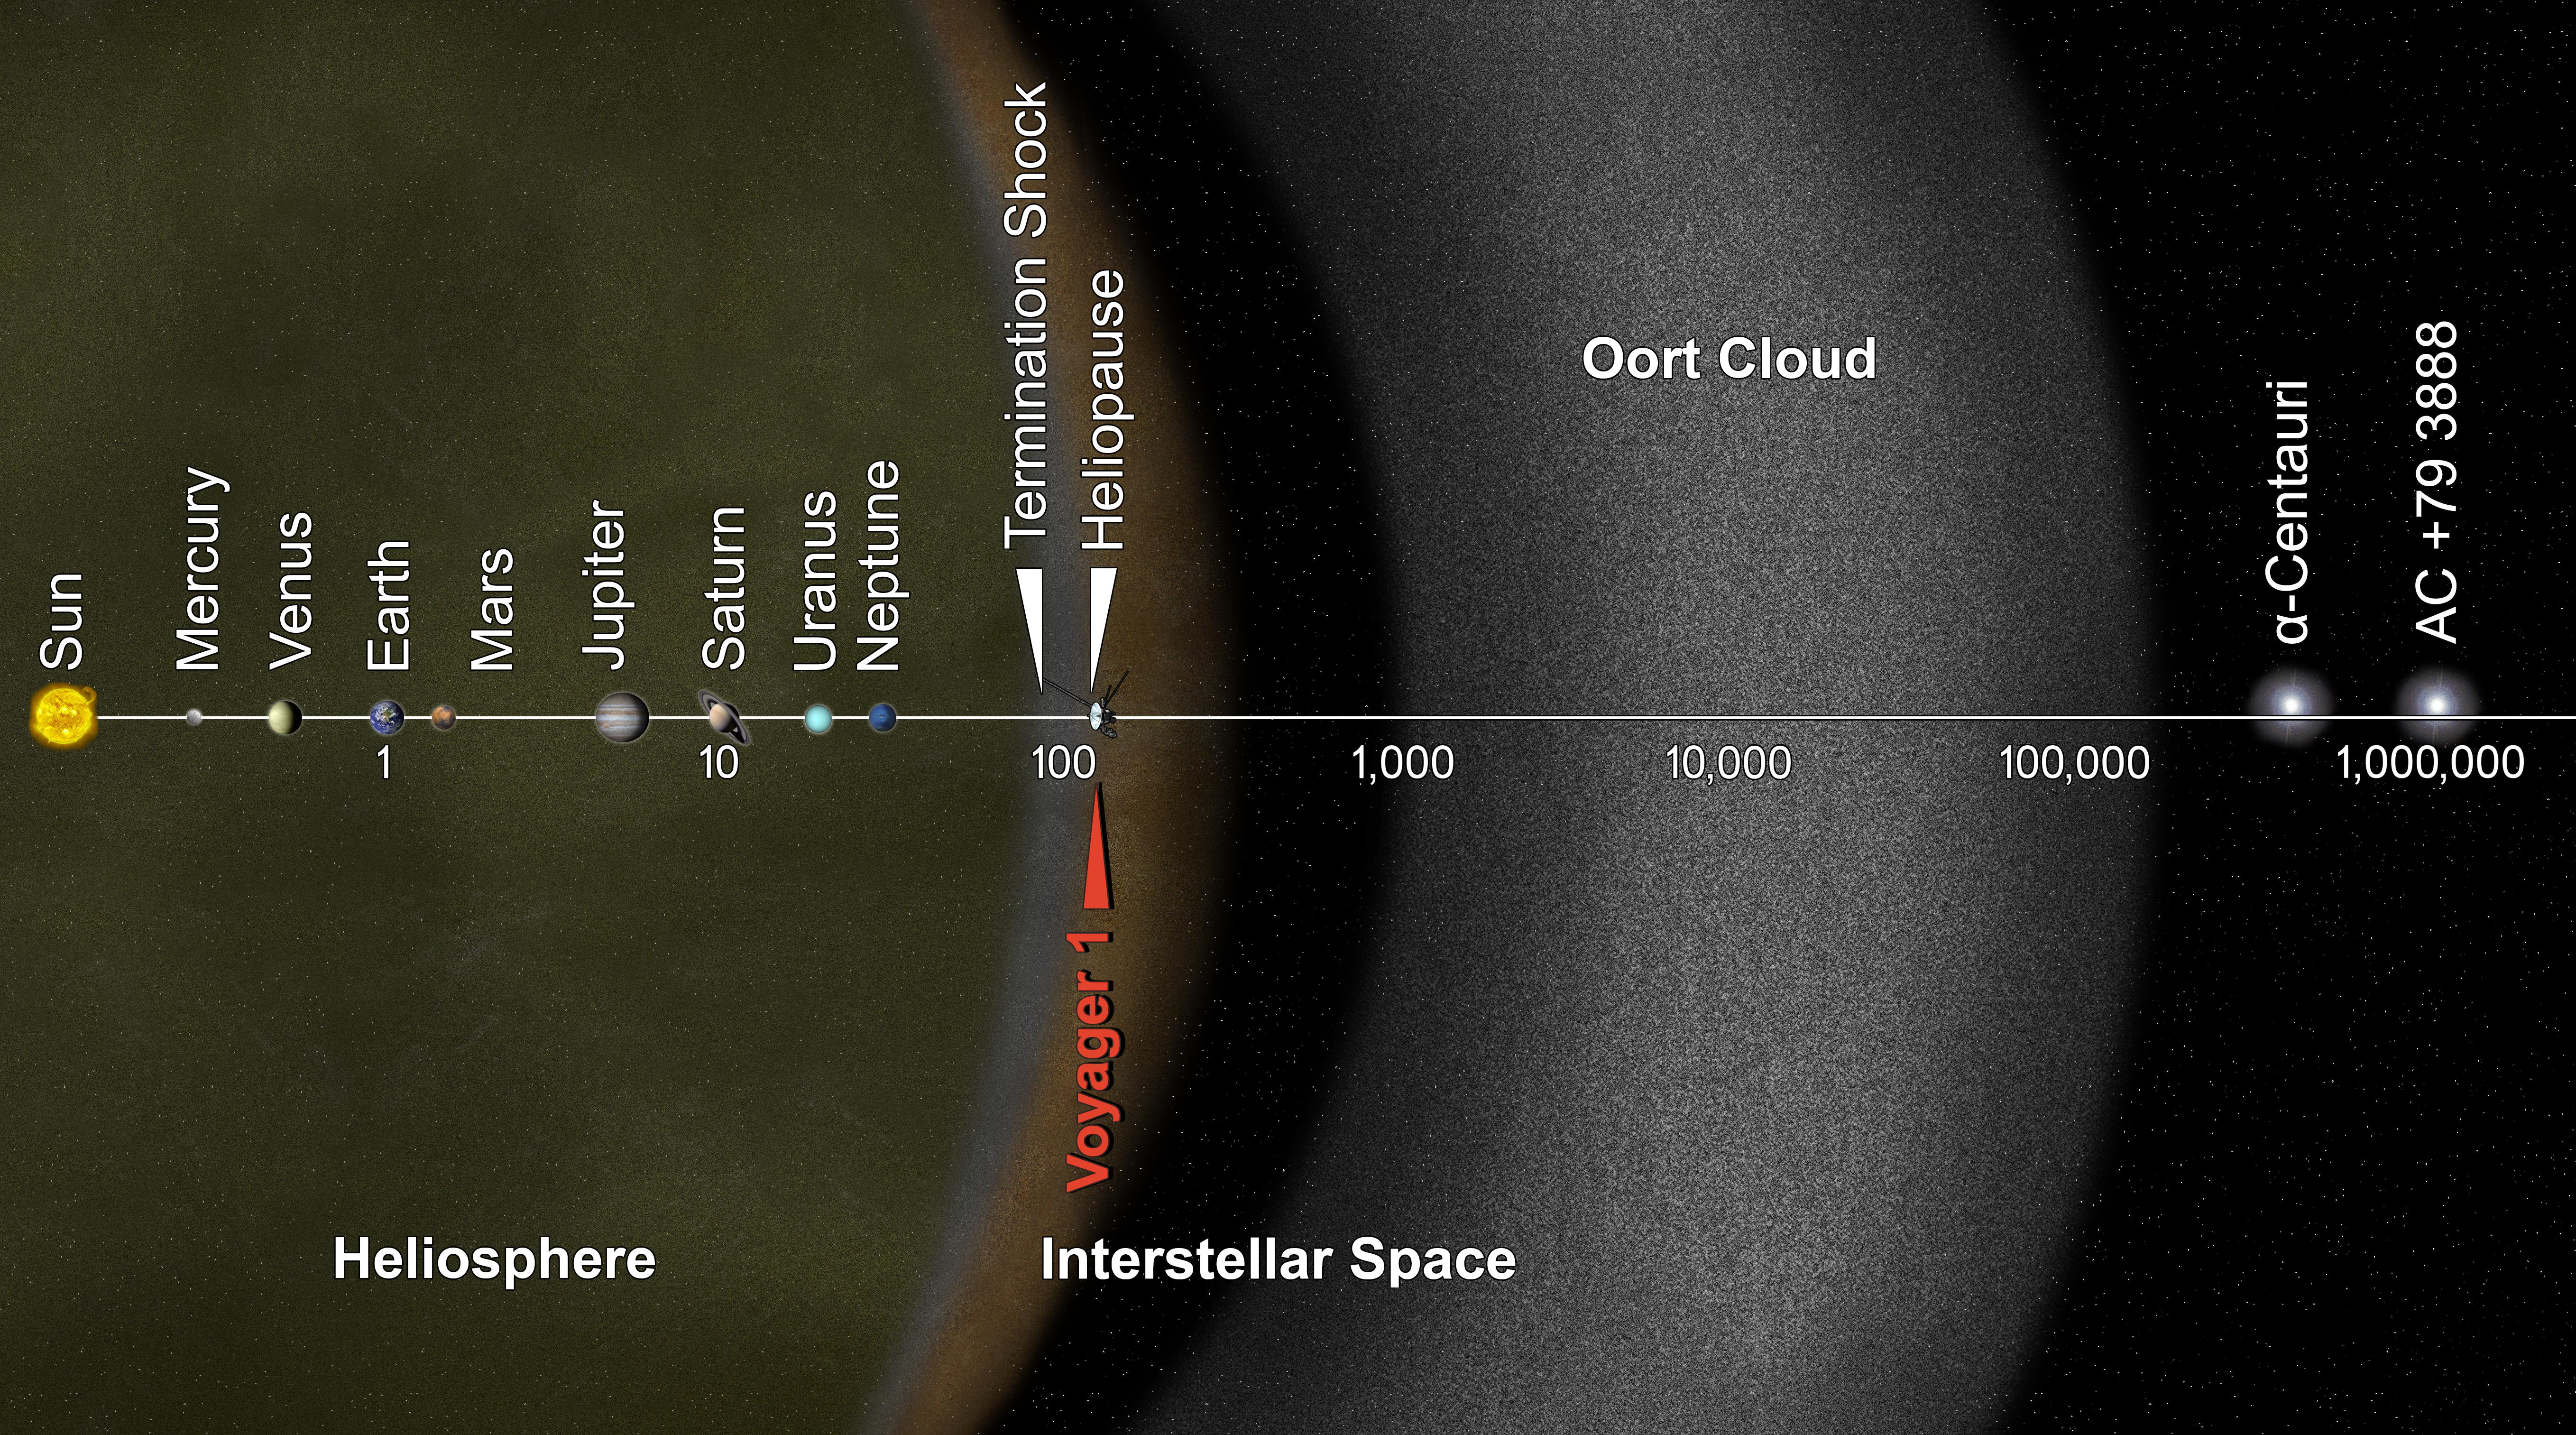
\includegraphics[height=0.35\textheight]{fig/oortcloud}
	\caption[Oort cloud]{Oort cloud - By NASA / JPL-Caltech}
	\label{oort}
\end{figure}

The Oort cloud is theorized to contain many millions of asteroids and long period comets. It is
far enough from the sun that it encircles the solar system in a sphere rather than lying within
the solar plane like the planets. Due to this, any future probe trying to access deep space
beyond our own system will need to account for the existence of the Oort cloud, regardless of
the direction of travel. A probe to verify its existence and to take asteroid number density
measurements will allow us to begin planning extra-solar voyages in the future. Spacecraft run
a serious risk of bombardment when traversing the Oort cloud, and experimental verification of
its existence would allow us to assess the risk of extra-solar missions more accurately. The
added benefit of Oort Cloud exploration is the ability for onboard instruments to take
measurements as it transits. More data on planets like Jupiter and Pluto could be obtained, and
deep space measurements far from planetary influences could also be taken.

Bimodal nuclear reactors for space power propulsion and electricity generation consequently appears to be the main solution to complete the mission.


\section{Reactor Design Options}

Two broad design categories have been considered throughout history for space nuclear reactor programs, direct propulsion and electric propulsion. Direct propulsion consists in ejecting a high speed jet of gas from the rocket, similar to a chemically-propelled system. Electric propulsion uses the electricity converted from the power source to power the thrusters. Within these categories, different system have been developed to various degrees of experimental testing. The main designs options seen in the contemporary literature are Gas Cooled Reactors, Heat Pipe Cooled Reactors and Liquid Metal Cooled Reactors.

\subsection{Liquid metal cooled reactors}

Several design using liquid metal as a coolant have been proposed. The LM-concept developed in 2003 used Lithium as a coolant~\cite{weitzberg2003liquid}. It aimed at delivering 100 kWe for over ten years and was based on electrical propulsion. The goal of this concept was to reuse as much components and research from SP-100 projects as possible~\cite{weitzberg2003liquid}. The SCoRE reactor concepts displayed in Figure~\ref{SCoRE} use a liquid metal coolant in a compartimentalized design avoiding single point failures, in order to mix the reliability advantages of a heat pipes system with the simplicity of a liquid metal cooled design~\cite{el2005score}. The core is divided into six zones, neutronically coupled but thermal-hydraulically independent.


\begin{figure}[]
	\centering
	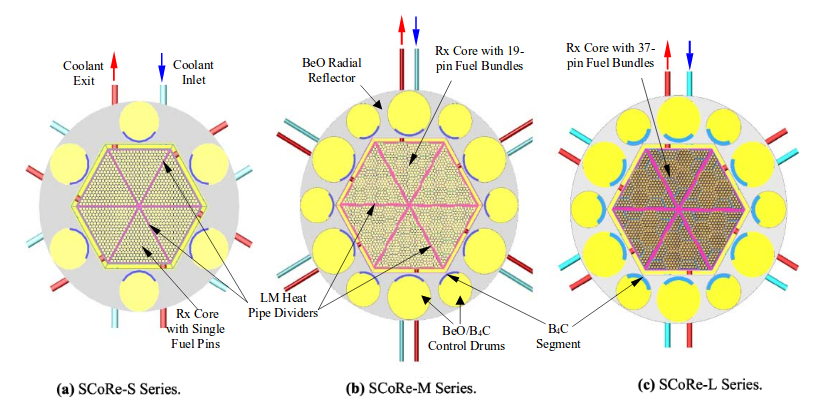
\includegraphics[height=0.35\textheight]{fig/SCoRE}
	\caption[Reactor Core Radial Cross-Sections of SCoRe Concepts]{Reactor Core Radial Cross-Sections of SCoRe Concepts, not to scale~\cite{el2005score}}
	\label{SCoRE}
\end{figure}


\subsection{Heat pipes cooled reactors}
\label{heatpipe}

The heat pipes design for space power application was developed by Los Alamos since 1994~\cite{poston2001heatpipe}, with a goal of 100 kWe in a space environment for 7 years. Heat pipe reactors operate in a fast spectrum and are cooled by heat pipes with working fluid such as Lithium, in the case of the 1982 SP-100 design. Heat pipes designs offer a redundancy in the heat removal, which would avoid single point failure, an important consideration for a space mission. Heat pipes are a closed circuit containing a fluid. During the reactor operation, the fluid is evaporated, travel through the reactor, and is condensed at the end and transfer the heat~\cite{reid1999heat,dean1985heat}.

The Heatpipe-Operated Mars Exploration Reactor or HOMER and the Safe Affordable Fission Engine or SAFE are both systems that work off the heatpipe power system. These heatpipe power systems are designed to be bimodal~\cite{houts1997heatpipe}. The goal of heatpipe power systems are to be: safe, reliable, long lived, modular, testable, versatile, easily fabricable, able to store fuel separately, able to be built with existing technology, bimodal, dual use (civilian and military), low mass, low cost, and be quick to develop, meaning they work off existing technology~\cite{houts1997heatpipe}. These systems will use either UN or UO2 as fuel and have low burnup~\cite{houts1997heatpipe}. They typically operate around 1300 K and can use several different energy conversion systems~\cite{houts1997heatpipe}. If operating below 100 kWth, radiation heat can be adequately removed through finned heatpipes~\cite{houts1997heatpipe}. An example of a heatpipe power system is shown in Figure~\ref{appP}. 


\begin{figure}[]
	\centering
	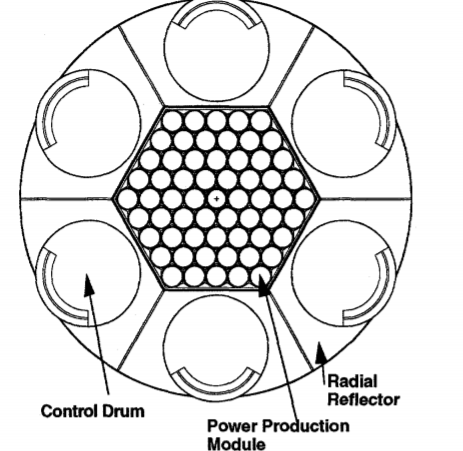
\includegraphics[height=0.45\textheight]{fig/appP}
	\caption[Heatpipe Power System Reactor Example]{Heatpipe Power System Reactor Example~\cite{poston2001heatpipe}}
	\label{appP}
\end{figure}

The HOMER system contains stainless steel clad UO2 fuel pins that are structurally and thermally bonded to SS/Na heatpipes~\cite{poston2001heatpipe}. The UO2 is 90\% theoretical density and 97\% enriched~\cite{poston2001heatpipe}. Heat is transferred from the fuel pins to the heatpipes, and the heatpipes move the heat to an out-of-core power conversion system, so there is no pumped loop system~\cite{poston2001heatpipe}. It is designed to stay sub-critical even if submerged in water~\cite{poston2001heatpipe}. For a 20 kWe HOMER system assuming 20\% conversion efficiency, the core needs 57 heatpipes, 152 fuel pins which results in 128 kg UO2, and 8 BeO pins, with a total reactor mass of 385 kg~\cite{poston2001heatpipe}. Heat would be removed with a radiator and the shielding is dependent on the type of mission. The mass distribution for this system in shown in Figure~\ref{appQ}. 


\begin{figure}[]
	\centering
	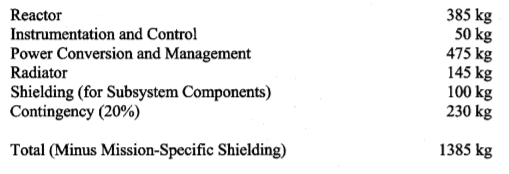
\includegraphics[height=0.15\textheight]{fig/appQ}
	\caption[HOMER Mass Breakdown]{HOMER Mass Breakdown~\cite{poston2001heatpipe}}
	\label{appQ}
\end{figure}

The SAFE-400 is a specific SAFE reactor that produces 400 kWth and uses a Brayton power system to get 100 kWe~\cite{poston2002design}. The core consists of 127 Mo modules and a Mo/Na heatpipe is at the center of each module surrounded by three Mo tubes that contain rhenium clad UN~\cite{poston2002design}. The UN is 96\% theoretical density and 97\% enriched~\cite{poston2002design}. Mo is chosen because of its high strength at high temperatures, its high thermal conductivity, and its good neutronics properties~\cite{poston2002design}. However, Mo is also difficult to make and weld, does not have a lot of information in the US irradiation database, and it brittle at low temperatures~\cite{poston2002design}. The reflectors and control drums are composed of Nb-1Zr clad Be~\cite{poston2002design}. Unlike the HOMER, the SAFE-400 uses a heatpipe to gas heat exchanger~\cite{poston2002design}. In general, this heat exchanger gas is made of 72\% He and 28\% Xe~\cite{webworldnuclear}. An example of the reactor core is shown in Figures~\ref{appR1} and~\ref{appR2}. Like the HOMER systems, the SAFE systems remain subcritical even when submerged.



Other more recent design have been proposed. The SAFE series, with notably the SAFE-400 concept~\cite{poston2002design} have shown great promises at nuclear eletric propulsion, coupled with a 100 kWe Brayton power system.


\begin{figure}[]
	\centering
	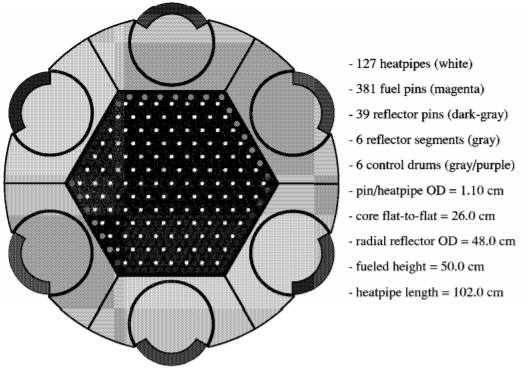
\includegraphics[height=0.45\textheight]{fig/appR1}
	\caption[SAFE-400 Reactor Design]{SAFE-400 Reactor Design~\cite{poston2002design}}
	\label{appR1}
\end{figure}


\begin{figure}[]
	\centering
	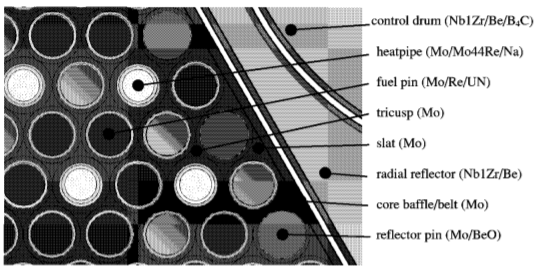
\includegraphics[height=0.35\textheight]{fig/appR2}
	\caption[SAFE-400 Reactor Design - Detailed]{SAFE-400 Reactor Design - detailed~\cite{poston2002design}}
	\label{appR2}
\end{figure}

One issue identified with this design rest in the fuel swelling limiting the burnup. Better fuel materials need to be developed. Fuel materials options are dicussed in section~\ref{fuelmat} of this report. Fission gas can also be problematic from a pressurization view point as well as poisoning the core.

This type of reactor also presents a number of technical challenges. The integration would be complex, with the routing of the heat pipes. The mass would have to be increased to account for a bigger shield. Finally, the reactor would operate at very high temperatures, impacting the available alloys and their characteristics for the heat pipes~\cite{el2005score}. 

\subsection{Gas cooled reactors}

A pin-type gas cooled reactor was designed to operate at 100 kWe for at least seven years~\cite{wright2003pin}, using Helium and Xenon gas and being used as a nuclear electric propulsion system. Similarly to the SCoRE liquid metal reactor concept, the solid-core, gas-cooled, Submersion-Subcritical Safe Space ($S^4$) reactor was designed to avoid single point failure and approach the risk and reliability values of the heat pipes reactor systems~\cite{king2006solid,king2009thermal}. Reactivity control schemes were compared on this design~\cite{craft2011reactivity}.

Gas-cooled reactors are inherently less efficient and less integrable with energy conversion systems that require high heat fluxes~\cite{el2002performance,fraas1966comparison,dochat1992free}.

Project Timberwind was initially started as part of the Star Wars program but later transferred to the air force and lasted from 1987 to 1992. Its goal was to achieve a specific impulse of 1000 seconds and have a thrust to weight ratio of 25:1, as the last NERVA rocket had a thrust to weight ratio of around 5:1~\cite{haslett1995space}. Project Timberwind used a particle bed reactor, with 4 different designs ranging from 400 to 2,000 MW~\cite{ludewig1996design}. Generally, in nuclear rocket systems, a high propellent pressure is needed to overcome the high pressure drop that occurs in the core~\cite{ludewig1996design}. This is why a pressurized bed reactor was chosen, as fuel elements composed of randomly packed spheres can minimize the pressure drop across the bed~\cite{ludewig1996design}. An example of the particle beds and the fuel it used are shown in Figure~\ref{appM}. Particle Bed Propulsion Reactors are heterogenous, have complicated symmetry, and have high neutron leakage, making analysis unique~\cite{ludewig1996design}. The most difficult issues were the temperature of the fuel (3500 K) and the thermal-hydraulic and structural performance of the fuel elements~\cite{haslett1995space}. The Soviet Union had created a mixed carbide fuel that was stable up to 4000 K~\cite{haslett1995space}. A slightly modified mixed carbide fuel was created, called the infiltrated kernel. It was lighter than mixed carbide fuel and performed better~\cite{haslett1995space}. An image of the fuel is shown in Figure~\ref{appN}. This fuel still had problems, when the UC2 became molten it would dissolve the buffer in five minutes and attack the ZrC coating, but the due to time and funding constraints, this issue was never fixed~\cite{haslett1995space}.


\begin{figure}[]
	\centering
	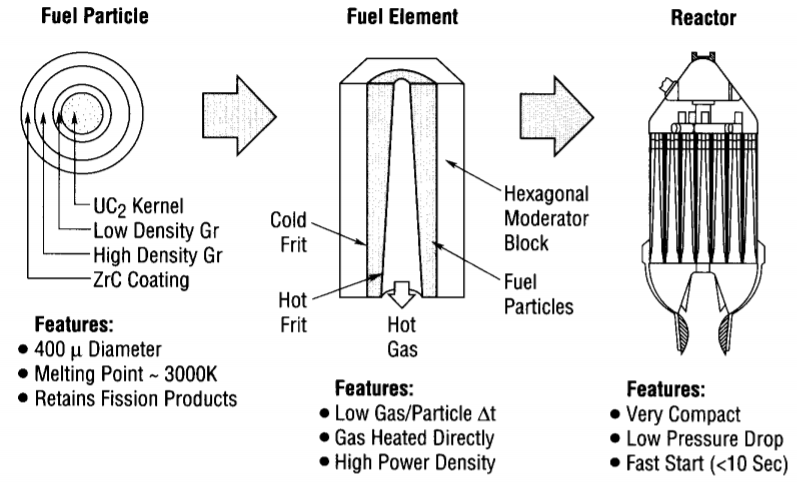
\includegraphics[height=0.45\textheight]{fig/appM}
	\caption[Project Timberwind's Fuel Particle, Fuel Element, and Particle Bed Reactor]{Project Timberwind's Fuel Particle, Fuel Element, and Particle Bed Reactor~\cite{ludewig1996design}}
	\label{appM}
\end{figure}

\begin{figure}[]
	\centering
	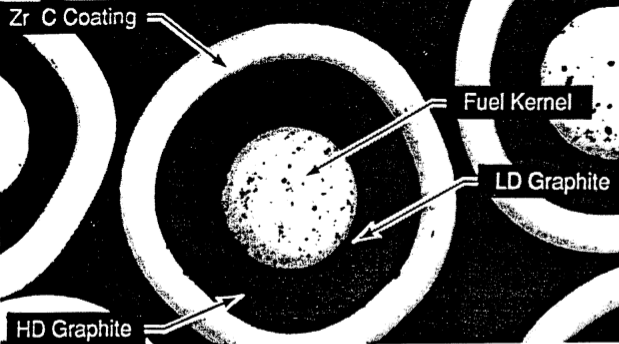
\includegraphics[height=0.35\textheight]{fig/appN}
	\caption[Infiltrated Kernel]{Infiltrated Kernel~\cite{haslett1995space}}
	\label{appN}
\end{figure}

The coolant, hydrogen, undergoes large temperature gradients, entering at 30 K and leaving at over 3,000 K~\cite{ludewig1996design}. The coolant enters the bed in a stainless steel cold frit and exits the bed in a TaC hot frit coated in graphite, with TaC being more durable than the traditional NbC~\cite{ludewig1996design}. The moderator used was Be/7LiH/H with a small Be reflector~\cite{haslett1995space}. The core consisted of 37 fuel elements, even though 61 fuel elements was superior from a neutronics standpoint, because it was much cheaper~\cite{haslett1995space}. 
There were 3 different Timberwind engines were designed but never tested or launched, Timberwind 45, 75, and 250~\cite{board2006priorities}. It was not fully declassified, but the 3 specifications of the target engines are shown in Table~\ref{appO}~\cite{board2006priorities}.

\begin{table}[]
\centering
\caption{Project Timberwind's Planned Specifications}
\label{appO}
\begin{tabular}{|l|c|c|c|}
\hline
\multicolumn{1}{|c|}{}         & Timberwind 45 & Timberwind 75 & Timberwind 250 \\ \hline
Diameter (ft)                  & 13.94         & 5.67          & 28.5           \\ \hline
Vacuum thrust (lbf)            & 99208         & 165347        & 551142         \\ \hline
Sea level thrust (lbf)         & 88305         & 147160        & 429902         \\ \hline
Vacuum specific impulse (s)    & 1000          & 1000          & 1000           \\ \hline
Sea level specific impulse (s) & 890           & 890           & 780            \\ \hline
Engine mass (lb)               & 3300          & 5500          & 8300           \\ \hline
Thrust to weight ratio         & 30            & 30            & 30             \\ \hline
Burn time (s)                  & 449           & 357           & 493            \\ \hline
Propellants                    & $LH_2$        & $LH_2$        & $LH_2$         \\ \hline
\end{tabular}
\end{table}

Various particle bed reactor designs cooled by a gas propellant have been developed for space nuclear thermal propulsion~\cite{hatch1960fluidized,ludewig1974feasibility,powell1985high}. The more recent PBR nuclear rocket aims at a specific impulse of 1000s and a competitive engine thrust/weight ratio with existing chemical rockets~\cite{ludewig1996design}.


\subsection{Fuel materials}
\label{fuelmat}

Over the years, several fuel options have been considered in a space nuclear power thermal rocket, each with its own set of advantages and inconvenients. No one option clearly demonstrated superiority over its competition. Different fuel choices can be considered, mainly in terms of neutron spectrum and fuel enrichment.

First, cermet and composite fuel will be considered. Next, HEU and LEU will be compared based on existing research. The research related to the spectrum used in various proposed design will then be considered, and finally tied to potential coolants.

\subsubsection{Fuel material types}

In Nuclear Thermal Propulsion (NTP) cores, mainly two types of fuel have been researched, composite and cermet. A third type has been considered, uranium nitride (UN) forms~\cite{matthews1993fuels}. Composite fuels are a carbon-based mixture of uranium with a material such as zirconium. Cermet fuels are a mixture of ceramic, usually tungsten, and uranium dioxide. The main strength of composite fuels resides in their neutronic properties, while cermet fuels have excellent thermal and material properties~\cite{postoncermet}, but lower neutronic performances due to the tungsten large absorption cross section~\cite{venneridesign}. Graphite-based fuel have been extensively tested during the NERVA and ROVER projects~\cite{taub1975review,lyon1973performance}. Cermet fuel experiments have been limited, but some informative failure data has been published~\cite{stewart2013comparison}.

More research is needed into both types of considered fuel, in order to assess their capabilities and their potential performance within an NTP system~\cite{qualls2017steps}.

\subsubsection{Fuel enrichment}

For a long time, high enriched uranium fuel was thought to be necessary, in order to have a high-energy reactor while minimizing the size. It was believed that highly enriched uranium (HEU) cores would always allow for more compact reactor designs, one of the goal for a potential use as space power~\cite{patel2016comparing}. This fuel however comes with two main disadvantages. Due to the use of HEU, any related research would have to be under strict national government review, barring market entry to private companies, and the risk of proliferation would be non-negligible~\cite{venneri2015feasibility}. The use of low enriched uranium (LEU) would consequently lower the global cost of a project and facilitate development~\cite{houts2014safe}.

The neutron economy in a HEU-fueled reactor is high, since most of the uranium is now fissile. This means that the probability of fissioning uranium is high enough that the neutron spectrum does not need to be softened much and the parasitic absorption by various core material is of lower concerns.

However, in recent years, it was shown that LEU fuel could demonstrate similar performance as HEU fuel nuclear thermal porpulsion system~\cite{ii2016engine,patel2016comparing}. NASA estimates that LEU fuel might be the only path toward a game-changing operative NTP system~\cite{houts2017low}.

Several preliminary designs using LEU have been proposed. One preliminary design showed the performance of using tungsten-cermet fuel~\cite{venneri2013nuclear}. A simple homogeneous model was modelled to compare a variety of fuel types, ranging from lithium hydride to zirconium hydride with uranium metal fuel~\cite{lee2015neutronic}. KANUTER-LEU was developed to be a small-size NTP system~\cite{nam2016preliminary}.

Interestingly, thorium was not considered as a potential fuel for a NTP system. Research in fuel materials for space power application with a Thorium-Uranium cycle is lacking in the literature.



\section{Space Nuclear Power: A history}
\label{sec:bkgd}


Nuclear power was first introduced to the space industry in the mid 1950's as radioisotope thermoelectric generators, or RTGs~\cite{doe0071}. The main idea is to use the heat produced by decaying isotopes and turn it into electricity. The most common radioisotopes used are Plutonium-238, Polonium-210, Cesium-137, and Americium-241~\cite{kinglecture},~\cite{webworldnuclear}. Plutonium-238 is the most common material used, providing a decay heat of 0.56 W/g and having a half-life of around 87.7 years~\cite{webworldnuclear}. Thermocouples convert this heat into electricity, which is used to power the onboard instrumentation. The maximum thermocouple efficiency was only around 10\%~\cite{engler1987atomic}. RTGs have no moving parts, are relatively light weight, do not use solar power, and the fissions do not cause chain reactions, meaning these RTGs will be reliable in space and output relatively constant amounts of power~\cite{engler1987atomic}. In 1961, the United States launched its first RTG: The SNAP-3 which provided only 2.7 watts~\cite{doe0071}. Even though these RTGs are reliable and long lasting, they do not produce large amounts of power. For example, the Cassini mission to Saturn launched in 1997 used 3 RTG units which only provided 850 watts~\cite{doe0071}. If more power is required, such as sending people to Mars, another power source should be considered.

\begin{figure}[]
	\centering
	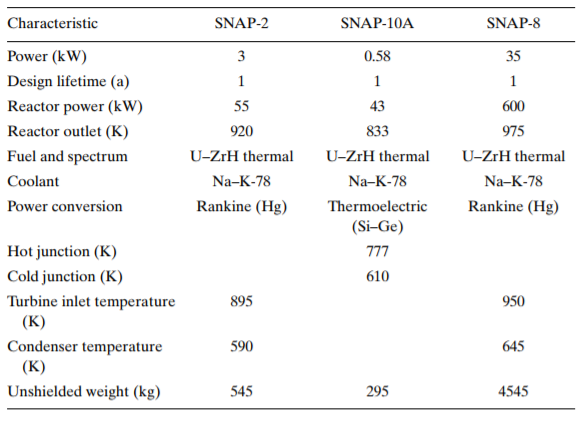
\includegraphics[height=0.35\textheight]{fig/img1}
	\caption[SNAP comparisons]{SNAP comparisons}
	\label{fig1}
\end{figure}

An alternative to RTGs and the main focus of this historical section will be on nuclear power from fission. The first United States program to implement fission was the Systems for Nuclear Auxiliary Power, or SNAP program, which started in the late 1950's. Various SNAP programs are compared in Figure~\ref{fig1}. The goal was to develop light, compact, and reliable atomic electric devices~\cite{voss1984snap}. This consisted of quite a few RTGs and four fission reactors: The SNAP Experimental Reactor or SER, SNAP-2, SNAP-8, and SNAP-10, with only the SNAP 10 reactor being fitted with a thermoelectric conversion system~\cite{websnap}. The SER used a hydride uranium-zirconium alloy enriched to 93\% U-235 as a fuel source, operating at 50 kWth~\cite{voss1984snap}. One of the advantages to this fuel is that the hydrogen acts both as the fuel and a moderator~\cite{voss1984snap}. This fuel was formed into rods and contained inside 0.01 inch thick stainless steel tubes~\cite{beall1962final}. These tubes were 0.975 inches in diameter and 14 inches long total, with 1.5 inches of beryllium on the top and bottom of the fuel and 0.5 inches of stainless steel used as an end cap. A diagram of this fuel rod is shown in Figure~\ref{appA}. 61 of these rods were arranged in a hexagonal shape to form the core, with six beryllium shims used to fill void space and act as a reflector~\cite{lords1994snap}. A diagram of the core is shown in Figure~\ref{appB}. There were three control drums used, which could not be scrammed, to control reactivity by changing reflectivity surface, with a maximum insertion rate of 2.5 cents/s and a total worth of \$3.82 over a 180$^{\circ}$ range~\cite{lords1994snap}. Three safety elements with around \$5.40 in reactivity each and a maximum insertion rate of 6 cents/s could be scrammed through releasing magnet power~\cite{lords1994snap}. The system was cooled with eutectic NaK containing 78 wt\% potassium, which had an outlet temperature of 1200$^{\circ}$F~\cite{beall1962final}. The main goal of the SER was to determine stability and safety of the reactor~\cite{voss1984snap}. Criticality was achieved and the reactor was operated for around 6,000 hours, with no visible damage from operation seen in the fuel rods, so the SER was considered a success~\cite{beall1962final}.  However, there were some problems that needed to be addressed. There was a problem with heater bundles in the secondary coolant loops failing, with three total failings across 11 months of testing. Noise could cause scrams to be initiated, and thermocouples were constantly failing.

\begin{figure}[]
	\centering
	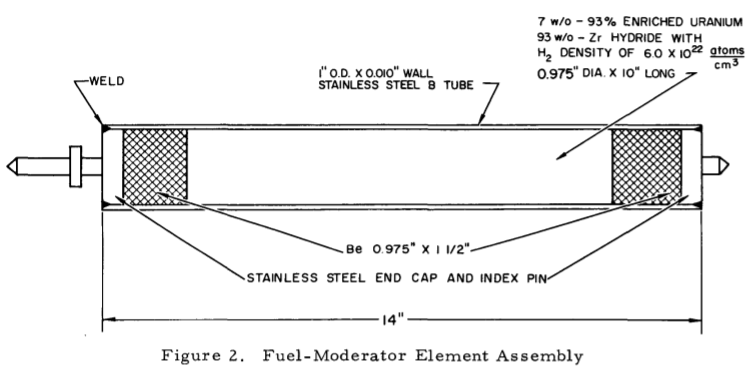
\includegraphics[height=0.35\textheight]{fig/appA}
	\caption[SER Fuel rod]{SER Fuel rod~\cite{lords1994snap}}
	\label{appA}
\end{figure}

\begin{figure}[]
	\centering
	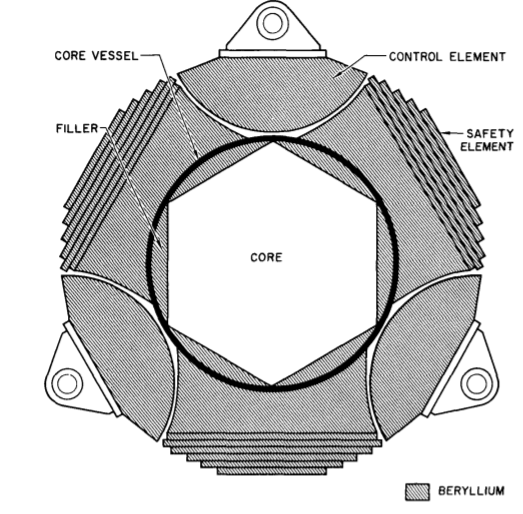
\includegraphics[height=0.45\textheight]{fig/appB}
	\caption[SER Coe Configuration]{SER Coe Configuration~\cite{lords1994snap}}
	\label{appB}
\end{figure}


SNAP-2 produced around 55 kWth, which was predicted to output 3.5 kWe using a Mercury-Rankine cycle~\cite{voss1984snap}. Unlike the SER, the SNAP-2 used 10\% enriched uranium, but ultimately kept the same hydride uranium-zirconium alloy as a fuel source~\cite{ohlenkamp1966snap}. It only had 37 fuel rods in total. There were no major problems during its lifetime, it was used to help characterize long term reactivity loss, xenon poisoning, and hydrogen redistribution~\cite{voss1984snap}. The SNAP-8 was a 600kWth reactor designed to produce 35 kWe with a maximum temperature of 1300$^{\circ}$F~\cite{daye1967snap}. After 1,000 hours of testing, the power was increased from 600 kWth to 1 MWth for 431 hours~\cite{voss1984snap}. This 1 MWth test resulted in 72 of 211 fuel elements cracking from stress due to fuel swelling at temperatures above design parameters~\cite{voss1984snap}. 


The SNAP-10A was the first and only nuclear reactor powered system that the United States launched. It was smaller than all the previous SNAP reactors in terms of power and weight. The SNAP-10A used the a hydrided uranium-zirconium alloy as a fuel~\cite{lords1994snap}.  Each fuel pin contained approximately 128g of U-235, 11.8g of U-238, 24.6g of H, and 1215g of Zr~\cite{voss1984snap}. A burnable poison of Sm2O3 was added to a few fuel elements in order to adjust the excess reactivity. The core had 37 fuel elements arranged in a triangular array, a beryllium reflector, and four semi-cylindrical drums with \$4.30 of reactivity each~\cite{voss1984snap},~\cite{ohlenkamp1966snap}. At launch, two of the control drums were inserted immediately and the other two were stepped in half a degree every 150 seconds, so the reactor would reach criticality seven hours after start up~\cite{voss1984snap}. Shielding was implemented in the form of lithium hydride cast inside a stainless steel case and weighed 98.6 kg~\cite{ohlenkamp1966snap}. The coolant was NaK at 1010$^{\circ}$F which was delivered at 13.2 gpm by a thermoelectric pump~\cite{ohlenkamp1966snap}. A honeycomb aluminum heat shield was used to keep the NaK above 75$^{\circ}$F during prelaunch so it wouldn't freeze and block the pipes~\cite{ohlenkamp1966snap}. PbTe thermoelectric elements were initially used for power conversion due to high performance, but had some disadvantages: high sublimation rates at high temperature and low strength and brittleness~\cite{voss1984snap}. They were replaced with SiGe alloyed thermocouples with lower performance, but had some advantages: low vapor pressure at high temperature, good mechanical integrity, and stability at temperatures greater than required on the SNAP-10A~\cite{voss1984snap}. No serious component failures were seen during the testing period, partly due to the redundancy in the system~\cite{ohlenkamp1966snap}. The total launch weight of the system was 436.4 kg and ended up producing over 600 We after launch on April 3rd, 1965~\cite{websnap}. After 43 days, the system shut down due to a high voltage failure~\cite{websnap}. The SNAP-10A reactor is shown in Figure~\ref{appC} with the thermodynamic cycle shown in Figure~\ref{appD}. 


\begin{figure}[]
	\centering
	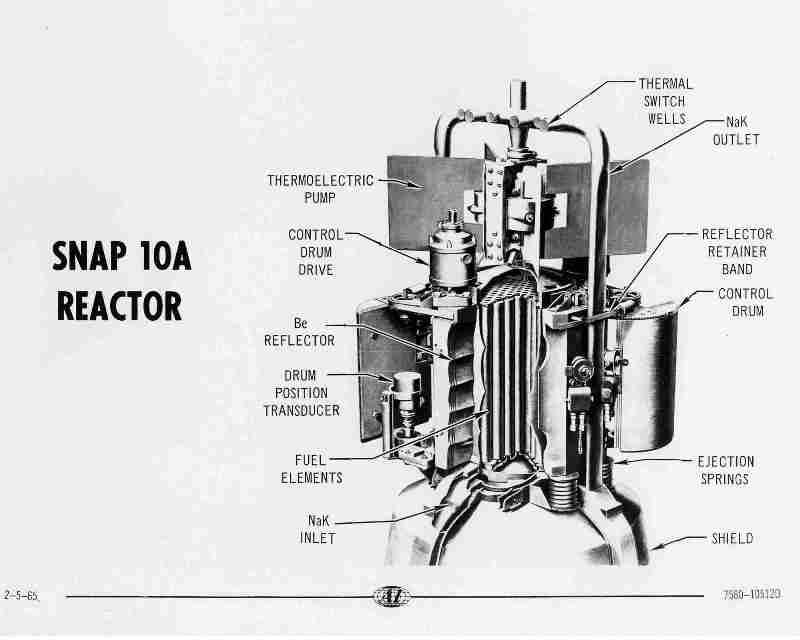
\includegraphics[height=0.45\textheight]{fig/appC}
	\caption[Cross section view of Snap-10A reactor]{Cross section view of Snap-10A reactor~\cite{websnap}}
	\label{appC}
\end{figure}


\begin{figure}[]
	\centering
	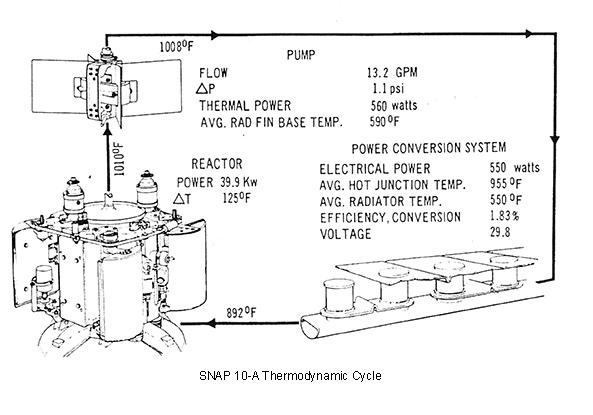
\includegraphics[height=0.45\textheight]{fig/appD}
	\caption[Thermodynamic cycle of SNAP-10A reactor]{Thermodynamic cycle of SNAP-10A reactor~\cite{websnap}}
	\label{appD}
\end{figure}



Even though it wasn't possible to test the SNAP-10A in the same conditions as space, no new environmental interactions were observed, so no modifications needed to be made to the system~\cite{ohlenkamp1966snap}. However, through the ground testing done, there were several systems or components that needed to be re-designed: such as the NaK pump, the thermoelectric modules, expansion compensator, and temperature switches~\cite{voss1984snap}. Even though the power output of the SNAP-10A was low, the systems created and research done is still relevant and reliable. For example the SiGe thermocouples were chosen despite not being the best for the SNAP-10A because of their predicted growth potential~\cite{voss1984snap}. 


The SP-100 space nuclear reactor was run from 1983 to 1992 with a projected power range of 10s to 100s of kWe for systems lighter than 3,000 kg that was operable at full power for seven years with an overall reliability of 95\%~\cite{borgesprimary},~\cite{anderson1983power}. The reactor was capable of making 2.4 MWth using 858 fuel pins and 3 safety rods~\cite{demuth2003sp100}. These fuel pins are arranged into a triangular lattice with a pitch to diameter ratio of 1.07, shown in Figure~\ref{appE}~\cite{el1992decay}. The safety rods are composed of a combination of B4C and BeO, shown in Figure~\ref{appF}~\cite{demuth2003sp100}. The core was cooled with liquid lithium which is coupled to 4 dynamic energy conversion engines, either a Brayton or a Stirling power converter~\cite{el1992decay}. For shielding, B4C and LiH were used for neutron shielding and depleted U was used for gamma shielding~\cite{demuth2003sp100}. A picture of the core is shown in Figure~\ref{appG} with a diagram of the fuel pins displayed in Figure~\ref{appH} and the shielding layout shown in Figure~\ref{appI}.


\begin{figure}[]
	\centering
	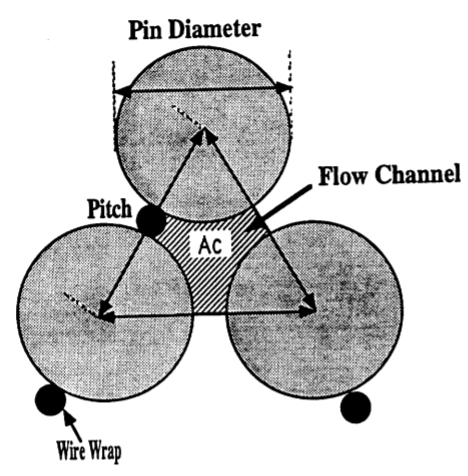
\includegraphics[height=0.45\textheight]{fig/appE}
	\caption[SP-100 Fuel Pin Lattice]{SP-100 Fuel Pin Lattice~\cite{el1992decay}}
	\label{appE}
\end{figure}


\begin{figure}[]
	\centering
	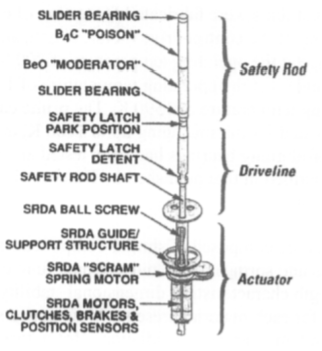
\includegraphics[height=0.45\textheight]{fig/appF}
	\caption[SP-100 Safety Rod Drive Assembly]{SP-100 Safety Rod Drive Assembly~\cite{anderson1983power}}
	\label{appF}
\end{figure}

\begin{figure}[]
	\centering
	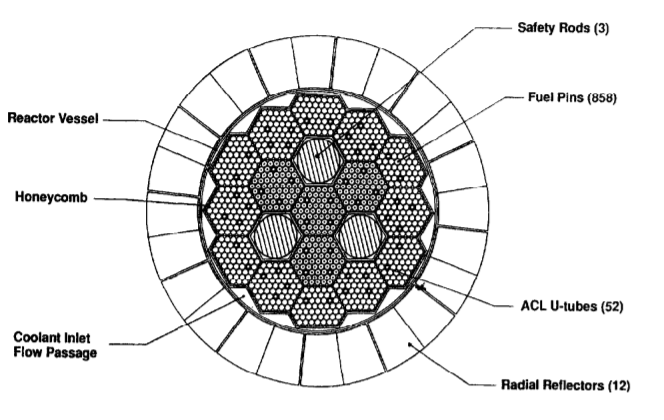
\includegraphics[height=0.45\textheight]{fig/appG}
	\caption[SP-100 core cross section]{SP-100 core cross section~\cite{anderson1983power}}
	\label{appG}
\end{figure}

\begin{figure}[]
	\centering
	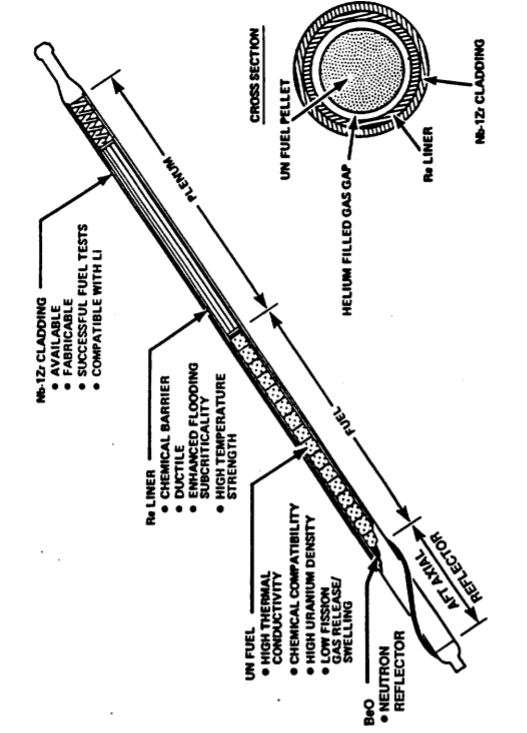
\includegraphics[height=0.45\textheight]{fig/appH}
	\caption[SP-100 Fuel Pin Configuration]{SP-100 Fuel Pin Configuration~\cite{el1992decay}}
	\label{appH}
\end{figure}

\begin{figure}[]
	\centering
	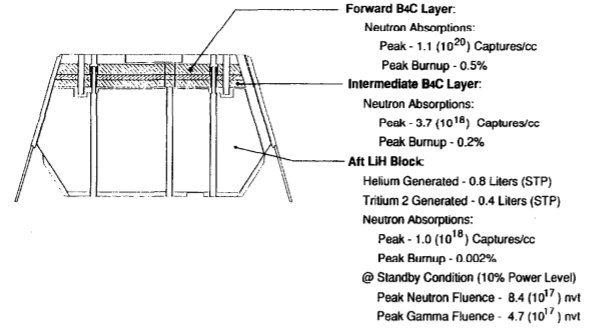
\includegraphics[height=0.45\textheight]{fig/appI}
	\caption[SP-100 Shielding Layout]{SP-100 Shielding Layout~\cite{anderson1983power}}
	\label{appI}
\end{figure}


As there were so many different constraints on this program, a few new things had to be done. Usually UO2 fuel is used in reactors, but because of the mass constraints UN was chosen instead, with a theoretical density of 94\% and enriched to 93.5\%~\cite{demuth2003sp100}. Some advantages to UN is that it has a high thermal conductivity, high uranium density, and low fission gas release~\cite{el1992decay}. Instead of stainless steel used as the fuel pin cladding a new material: bonded Nb-1Zr/Re was used~\cite{el1992decay}. This new material is more chemically inert with respect to the fuel and fission gases and is more compatible with the lithium coolant~\cite{demuth2003sp100}. Since the reactor needed to have a reliability above 95\%, the reactor was designed to~\cite{demuth2003sp100}:
\begin{enumerate}
\item Achieve full power with 1 heat rejection loop inoperative
\item Achieve full power with 1 control reflector stuck open
\item Have redundancy in the safety rod motors, brakes, and clutches
\item Accommodate fission gas leakage due to failure of 1\% of the fuel pins
\item Have excess thermoelectric area to account for lifetime degradation
\item Have a minimum of 2 circuits each with 2 sensors for every signal of critical importance
\end{enumerate}

For safety, the reactor was designed to remain inactive after submerging and flooding the core and ensure the dispersion of radioactive materials upon reentry met the nuclear safety requirements~\cite{anderson1983power}.


Some of the problems encountered with the SP-100 were the materials and the coolant. Since UN was used as the fuel, other cladding materials needed to be used, which led to the invention of the rhenium lined Nb-1\% Zr cladding. There also needed to be mass minimizations, which is why UN was chosen as the fuel and Li was chosen as a coolant. For safety reasons, Li was to be launched as a solid and thawed later~\cite{anderson1983power}. Liquid lithium has a volume of more than 25\% the volume of solid lithium, and the entire vessel had to be designed around repeated freeze and thaw cycles~\cite{anderson1983power}. NaK, a more common coolant, was still used in auxiliary cooling and thawing system because of its lower melting point~\cite{anderson1983power}. The SP-100 was terminated early and was able to achieve its goal of 100 kWe, but had a final mass of 4600 kg~\cite{anderson1983power}.


The SNAP-10A and SP-100 were examples of what could happen if nuclear power was used for powering satellites. Nuclear power can also be used for propulsion and powering satellites at the same time, which would be bimodal systems. Two programs kicked off nuclear thermal rockets: Nuclear Engine for Rocket Vehicle Application or NERVA by the US Atomic Energy Commission and NASA, and Project Rover by the Los Alamos Scientific Laboratory. Project Rover was split into three different phases: Kiwi, Phoebus, and Pewee. However, the Pewee, for which the fuel elements environment and mass loss are displayed on Figure~\ref{appV} was only used to test new fuels, and they didn't try to maximize the specific impulses, so these reactors will be mainly skipped over~\cite{finseth1991rover}. NERVA's designs were based on one of the Project Rover's Kiwi systems. Both Project Rover and NERVA were terminated in 1972. One of the main attractions of nuclear rockets is that they can achieve more than twice the specific impulse of the best chemical rockets~\cite{finseth1991rover}. It also has the capability to start, stop, and restart if necessary, which chemical rockets cannot do~\cite{finseth1991rover}. The best nuclear rockets will have a high exit gas temperature and the propellent should have low molecular weight, meaning hydrogen is the best choice~\cite{finseth1991rover}. A table displaying all the reactors tested, the dates of the tests, the maximum power achieved, and the time at maximum power is shown in Figure~\ref{appJ}.

\begin{figure}[]
	\centering
	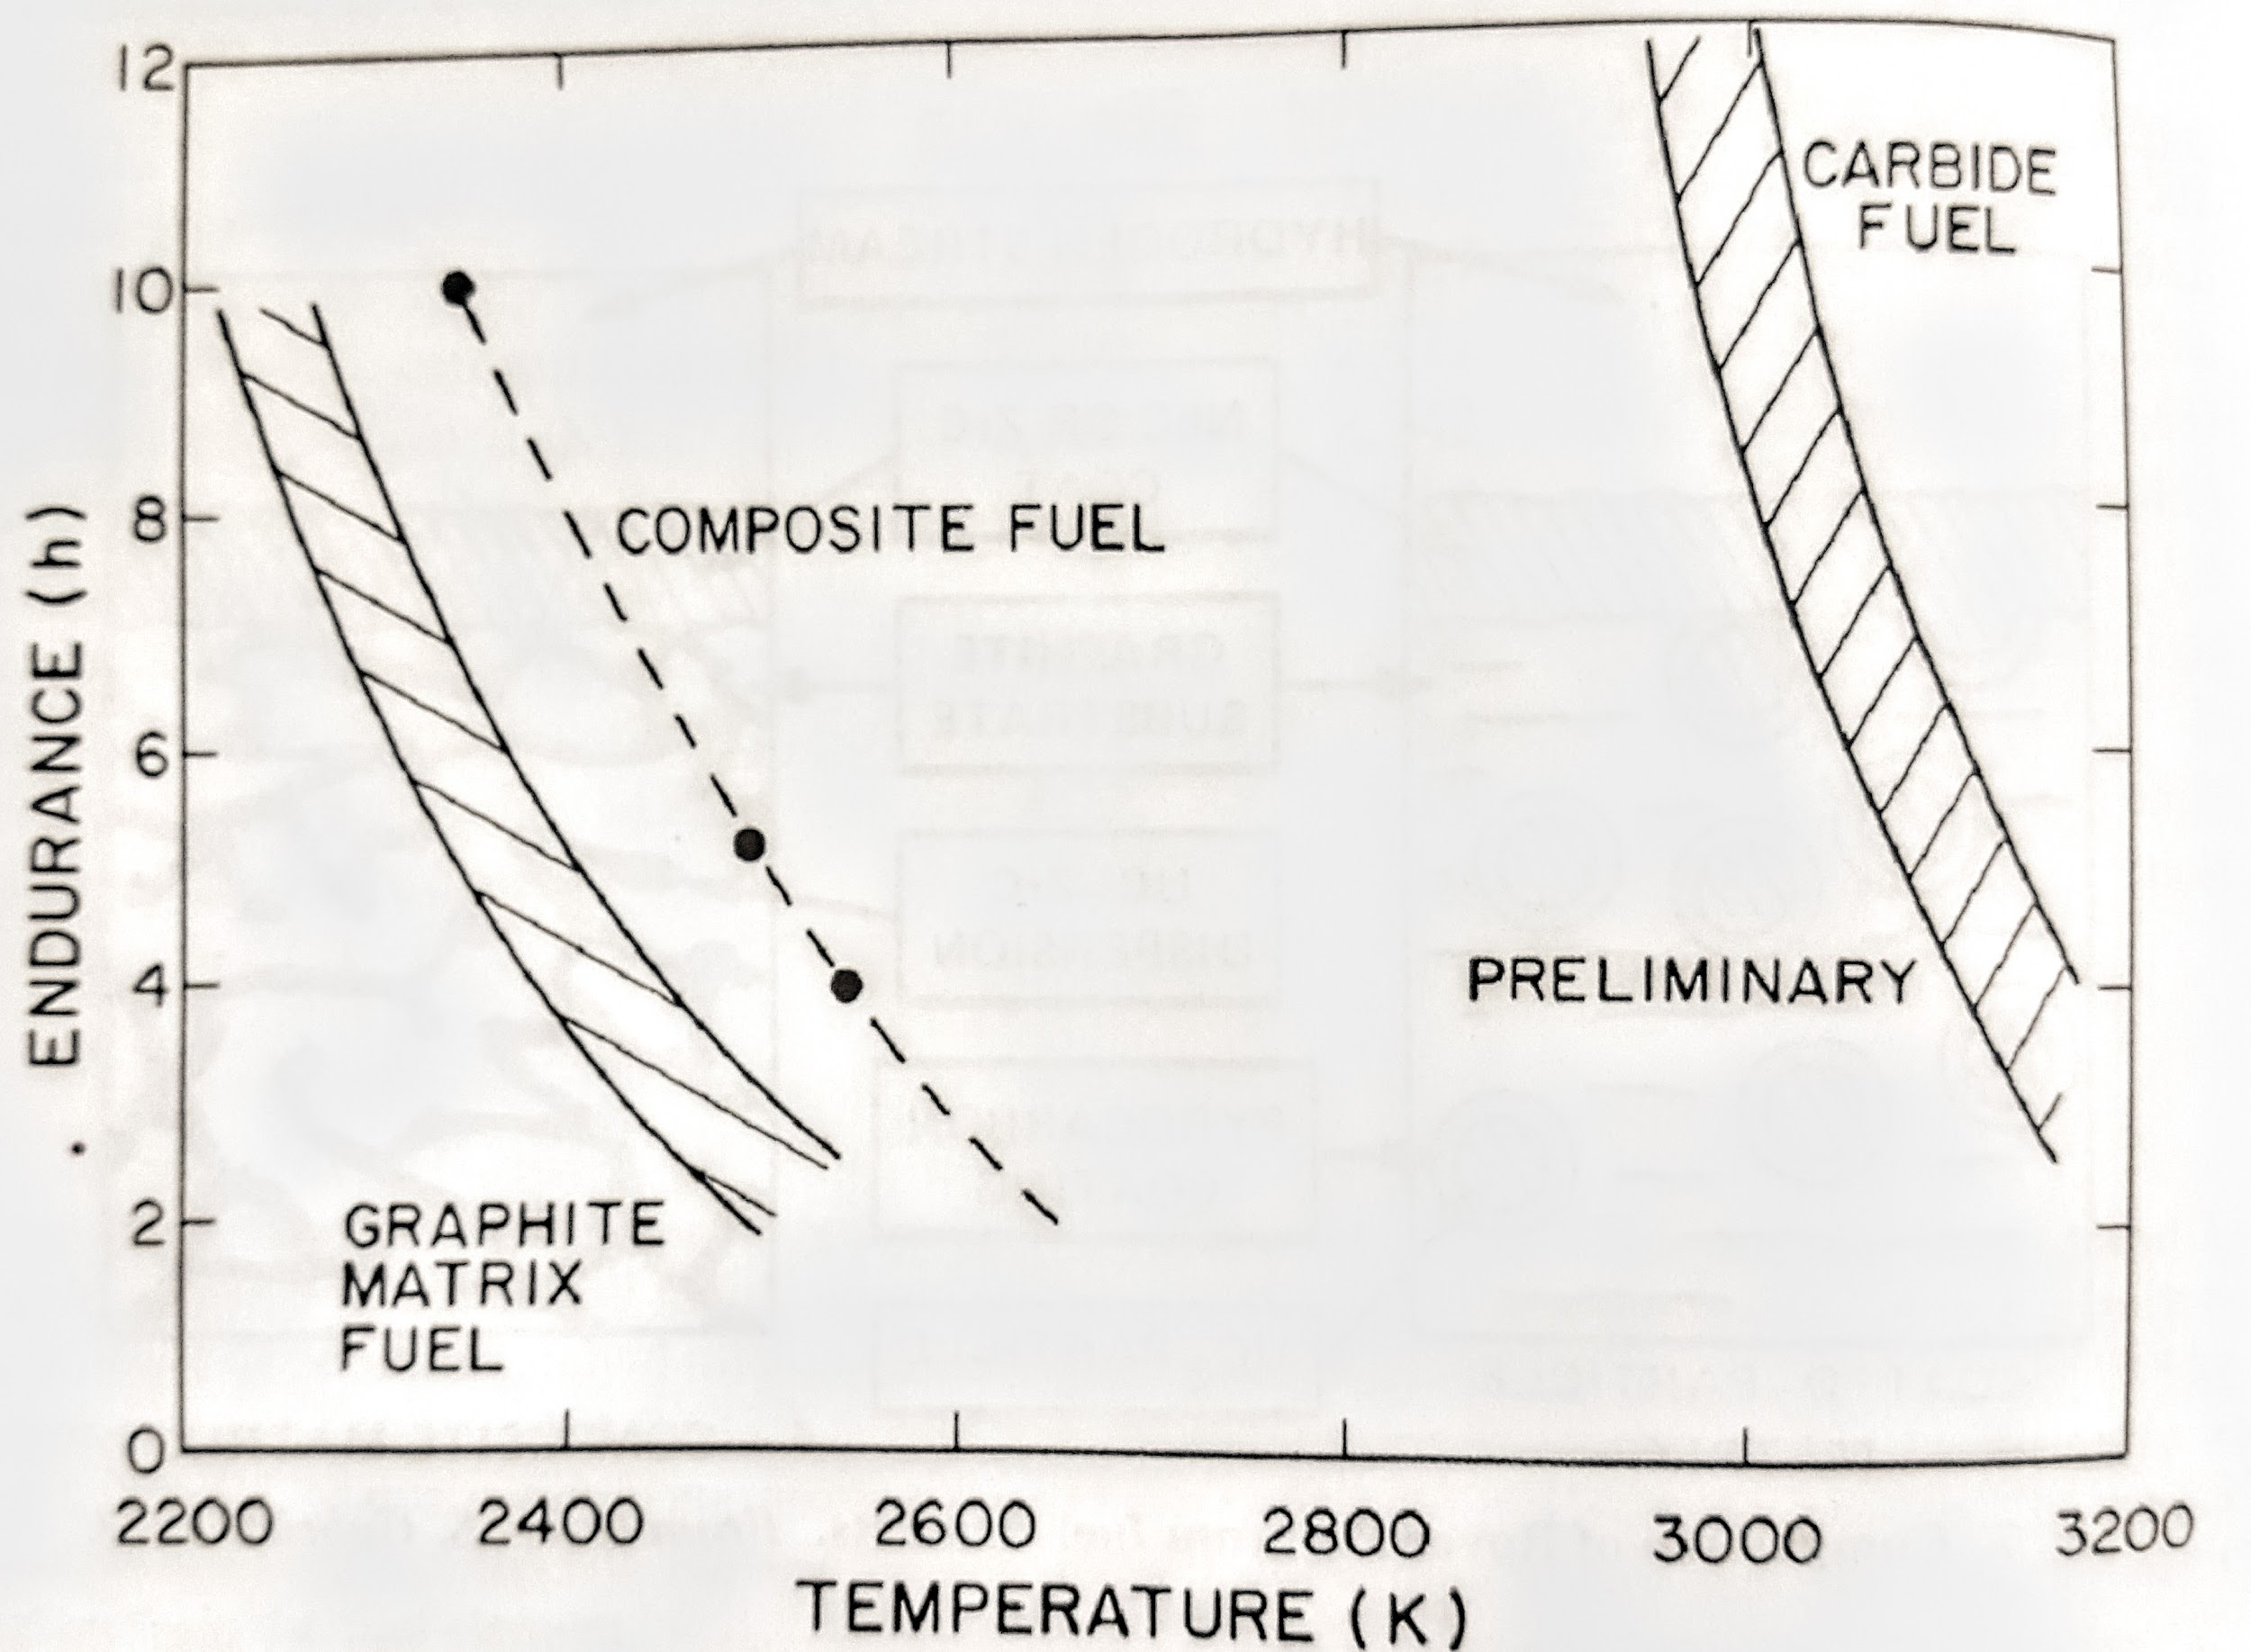
\includegraphics[height=0.45\textheight]{fig/appV}
	\caption[Fuel element environment and mass loss from Pewee and NF-1 fuels]{Fuel element environment and mass loss from Pewee and NF-1 fuels~\cite{lyon1973performance}}
	\label{appV}
\end{figure}

The Rover nuclear rocket schematics are displayed in Figure~\ref{appX}.

\begin{figure}[]
	\centering
	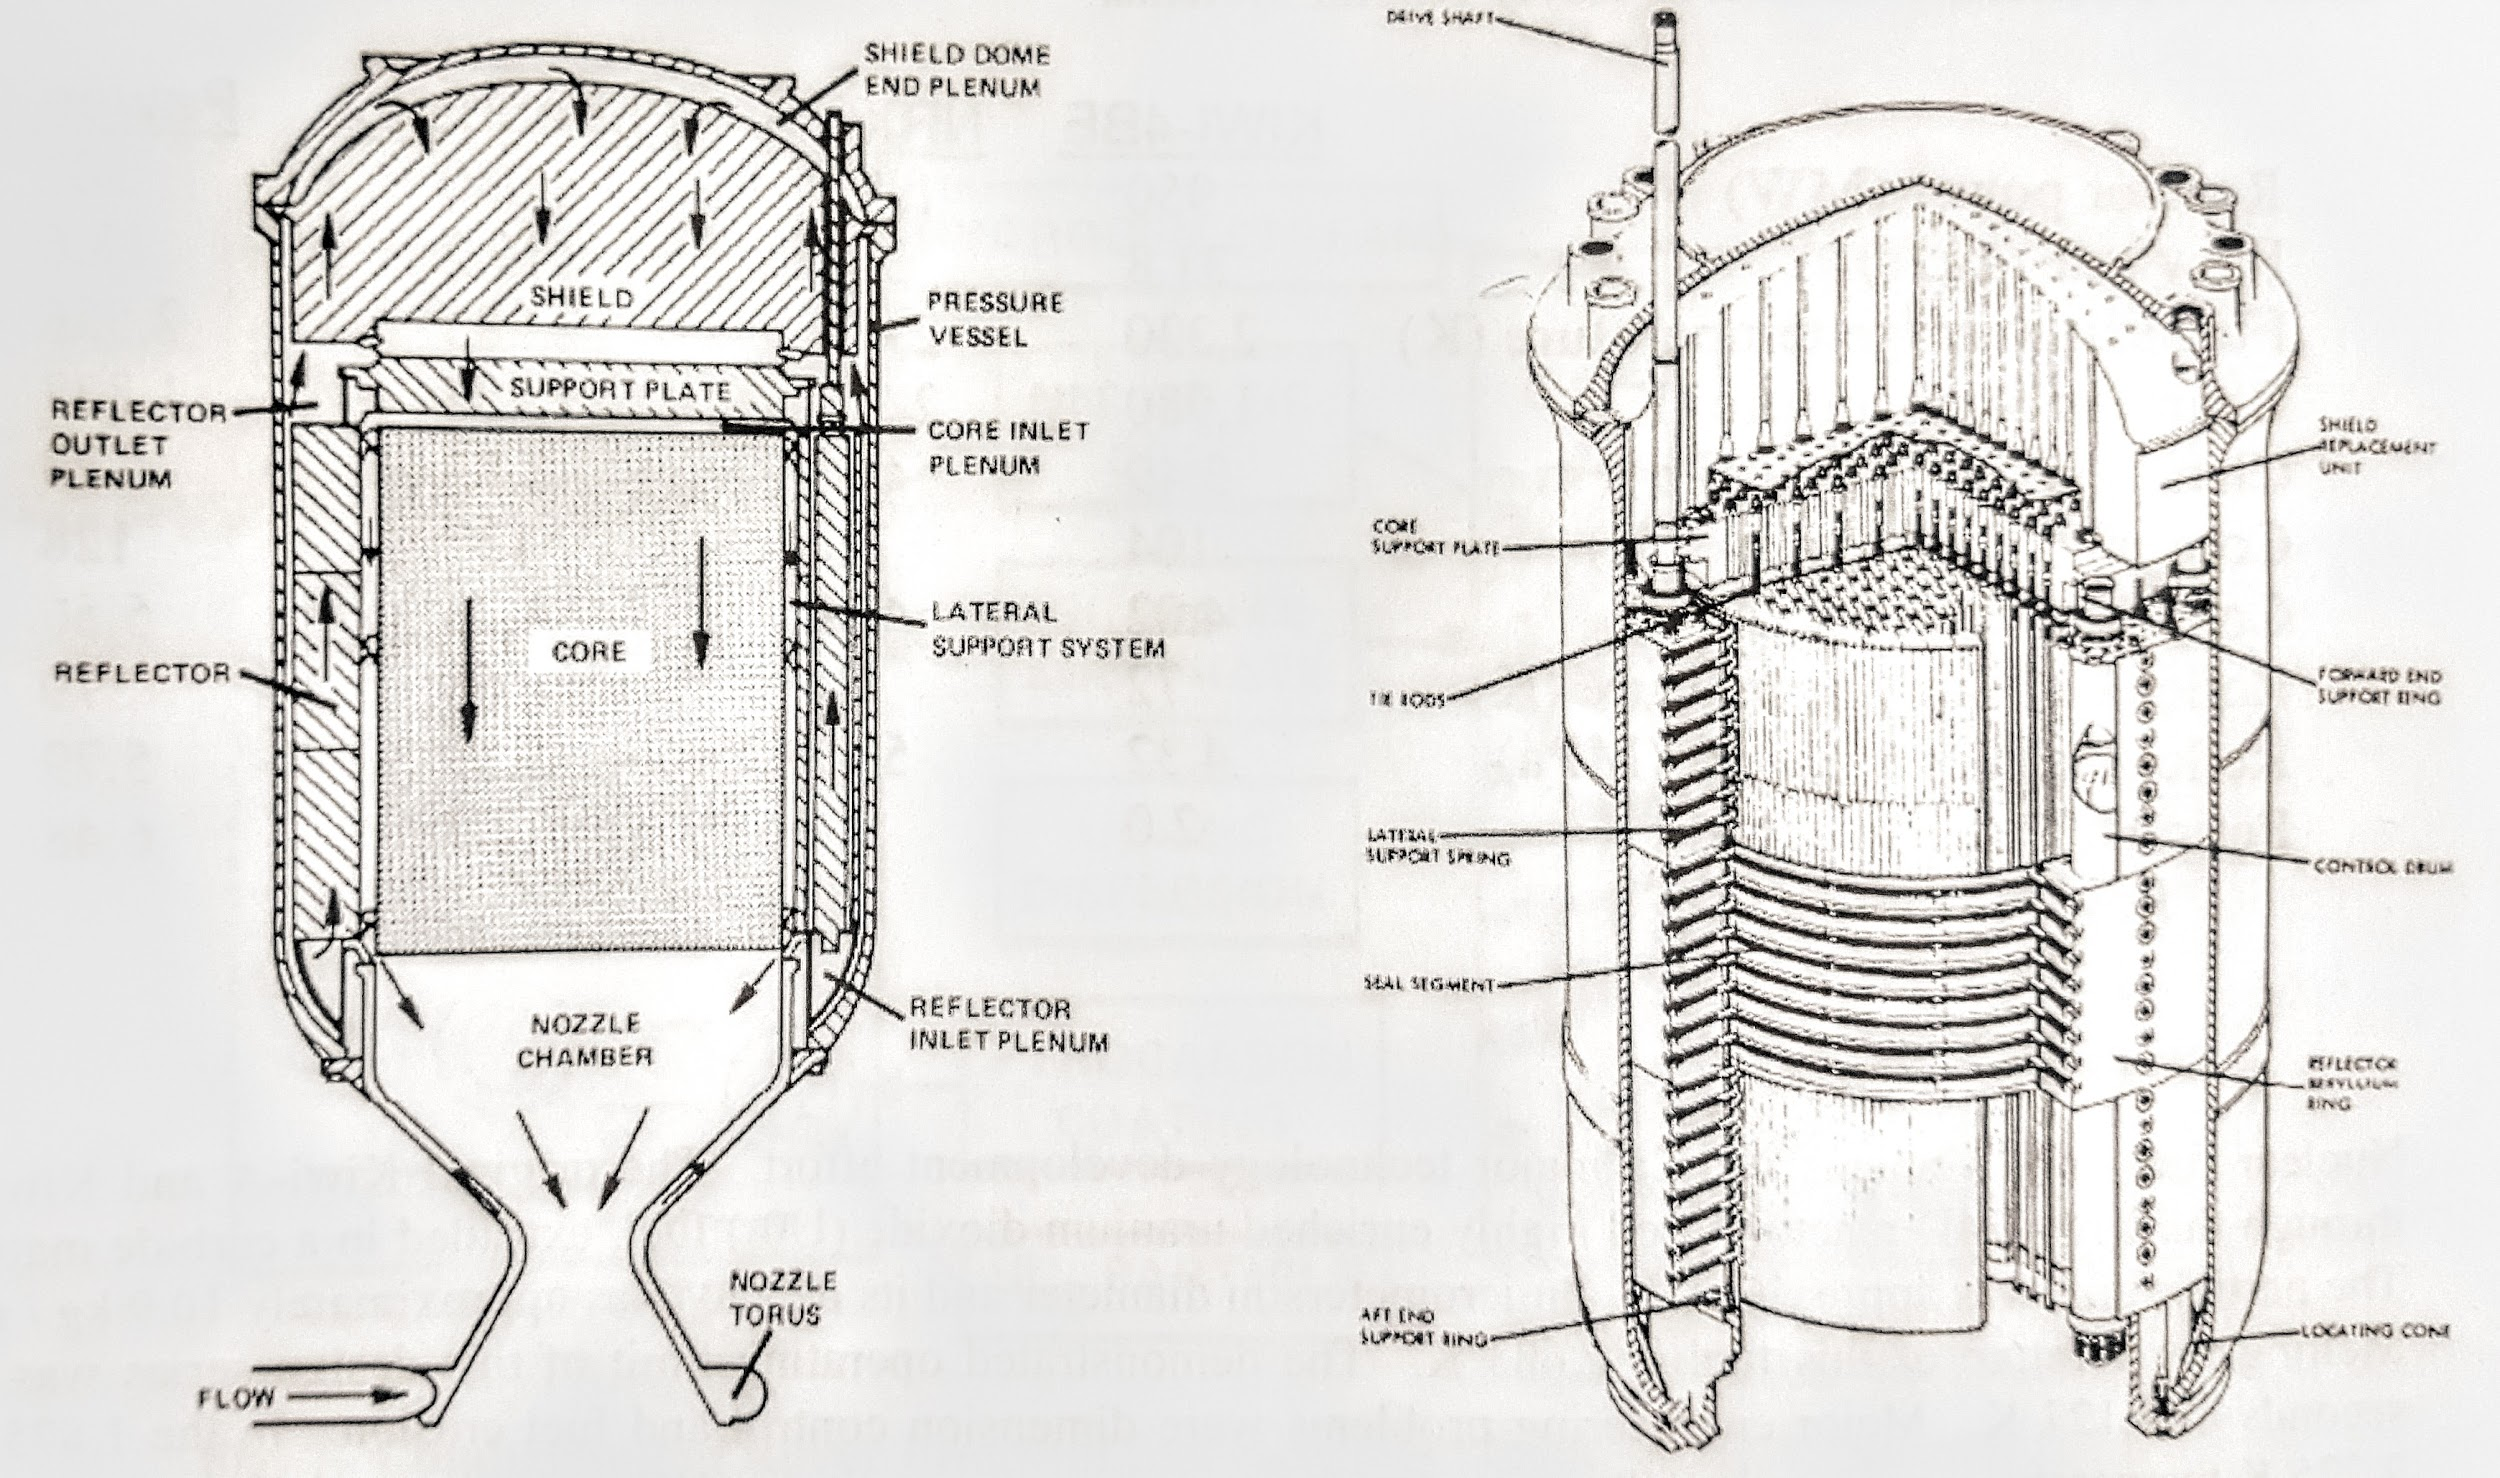
\includegraphics[height=0.45\textheight]{fig/appX}
	\caption[Schematic (left) and cutaway (right) of Rover nuclear rocket reactor]{Schematic (left) and cutaway (right) of Rover nuclear rocket reactor~\cite{wanl1613}}
	\label{appX}
\end{figure}



\begin{figure}[]
	\centering
	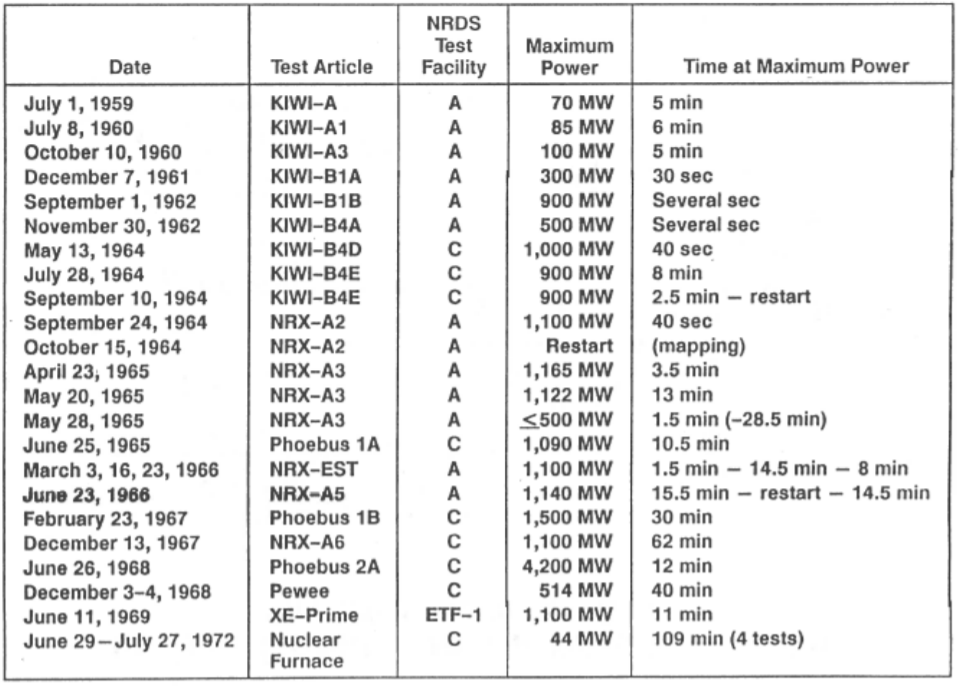
\includegraphics[height=0.45\textheight]{fig/appJ}
	\caption[Project Rover and NERVA Propulsion Tests]{Project Rover and NERVA Propulsion Tests ~\cite{gerrish2014nuclear}}
	\label{appJ}
\end{figure}

The Kiwi rocket had a total of eight different prototypes built and tested, but they were all epithermal reactors~\cite{finseth1991rover}. The Kiwi propulsion systems were split into two series: the Kiwi-A series and the Kiwi-B series~\cite{house1964development}. The main difference between these two was that the Kiwi-A series used gaseous hydrogen as its propellent and the Kiwi-B series used liquid hydrogen~\cite{house1964development}. The first Kiwi reactor tested was the Kiwi A reactor, which was tested in 1959~\cite{finseth1991rover}. This reactor was intended to produce 100 MW of power but instead achieved 70 MW and operated for 300 seconds~\cite{gerrish2014nuclear}. The propellent, gaseous hydrogen, left with a flow rate of 3.2 kg/s~\cite{finseth1991rover}. The nozzle was a double walled nickel, designed for sonic flow at the throat~\cite{finseth1991rover}. The fuel used was UO2 loaded graphite plates, used graphite as a reflector, and was encased in an aluminum pressure shell~\cite{finseth1991rover}. At high temperatures (around 2,000 K), the UO2 reacted with the surrounding carbon, converting it to UC2~\cite{finseth1991rover}. A graphite plate, which was supposed to contain the carbon wool insulation and prevent gas from bypassing, inside the reactor shattered during operation and was ejected out the nozzle~\cite{finseth1991rover}. This caused the gas outlet temperature to increase, which ultimately melted the UC2 that had formed, as it has a lower melting point than UO2~\cite{finseth1991rover}. Despite this, the test was still considered a success, as it showed the possibility of a high temperature nuclear propulsion reactor. 


The next Kiwi-A series reactor was the Kiwi A' reactor. This reactor also operated for around 300 seconds, but at a high power of 88 MW~\cite{gerrish2014nuclear}. One of the main differences between this reactor and the original Kiwi A reactor was the fuel. The Kiwi A' used UO2 fuel elements inside graphite modules which contained 4 coolant channels~\cite{finseth1991rover}. During operation, fuel modules were ejected from the core, but the reactor continued to operate at the designated power, with these ejection only causing short perturbations~\cite{finseth1991rover}. During the inspection after operation, it was found that 4 other fuel modules had cracks and would likely have also been ejected if it had been operated longer~\cite{finseth1991rover}. 

The last Kiwi-A series reactor was the Kiwi A3 reactor, which operated at just above 100 MW for around 300 seconds and was launched to test the structural integrity of different core materials at operating conditions~\cite{gerrish2014nuclear}. Nothing was ejected from the core during these tests, but some of the fuel elements were cracked~\cite{finseth1991rover}. The carbon wool insulation, core, and reflector were found to be in very bad shape as well~\cite{finseth1991rover}. Overall, the Kiwi-A series could be considered a success, as they were able to demonstrate a structurally sound reactor that could be precisely controlled and tested. 


The next reactors were the Kiwi-B series that mostly used liquid hydrogen as its propellent. The exception was the first reactor, the Kiwi B1A, which still used gaseous hydrogen~\cite{finseth1991rover}. This reactor was designed to be the same size as the Kiwi A, but output 10 times as much power~\cite{gerrish2014nuclear}. The Kiwi B1A achieved around 250 MW for around 30 seconds before a hydrogen fire near the nozzle stopped the test early~\cite{gerrish2014nuclear}. The average hydrogen mass flow at full power was 9.1 kg/s and the reactor achieved an ideal specific impulse of over 750 seconds~\cite{finseth1991rover}. Some of the major differences were a beryllium reflector, pyrographite as insulation, a regeneratively-cooled nozzle, 7 coolant holes per fuel element, hexagonal graphite modules, and fuel elements coated in NbC for corrosion resistance~\cite{finseth1991rover}. 


Kiwi B1B was the next reactor tested, and the first one to be tested with liquid hydrogen. It was rated for 1100 MW but only operated at around 900 MW for a few seconds~\cite{gerrish2014nuclear}. Its main objective was to investigate cryogenic hydrogen during reactor start up~\cite{finseth1991rover}. They were worried that the hydrogen may be flowing through as a 2-phase solution. Kiwi B1B's run was stopped early due to fuel elements being ejected from the core and small hydrogen fire started~\cite{finseth1991rover}. 11 modules were ejected and an addition 50 were broken, causing the B1B to stop being worked on~\cite{finseth1991rover}. The main differences between B1A and B1B were: there were more core periphery modules and it used full length fuel elements when the B1A used half-length elements~\cite{finseth1991rover}. 
The next reactor, the Kiwi B4A, had its run prematurely ended when it ejected its core~\cite{gerrish2014nuclear}. It used a new hexagonal fuel element with a flat to flat dimension of 0.75 inches and a length of 52 inches, which became the standard fuel element used~\cite{finseth1991rover}. This element used UO2 and had 19 coolant holes, and was coated in NbC for corrosion resistance~\cite{finseth1991rover}. It was later found that core vibrations from hydrogen flow caused the fuel elements to fracture~\cite{gerrish2014nuclear}. 


The Kiwi B4A's successor was the Kiwi B4D which aimed to eliminate these core vibrations. It reached full power at 1000 MW for around a minute before a hydrogen leak, which caused a fire, stopped the test early~\cite{gerrish2014nuclear}. This time, the fire didn't break any fuel elements and no mechanical damage was seen on the inside of the core~\cite{finseth1991rover}. The Kiwi B4D included leaf springs for lateral core support and was started completely automatically~\cite{finseth1991rover}. This reactor had a gas exit temperature of 2,222 K, a thrust of 45,851 lbf, and a vacuum specific impulse of 780 seconds~\cite{presrovernerva}.
The last Kiwi reactor was the Kiwi B4E which operated at over 900 MW for over 8 minutes, which was by far the most successful Kiwi iteration~\cite{gerrish2014nuclear}. The exiting gas temperature was 2,389 K with a propellent flow rate of 31.8 kg/s, a thrust of 45,851 lbf, and a vacuum specific impulse of 820 seconds~\cite{finseth1991rover},~\cite{presrovernerva}. It was operated again at almost 900 MW for another 2.5 minutes which confirmed the same gas temperature and propellent rate~\cite{finseth1991rover},~\cite{gerrish2014nuclear}. Two images of the reactor are shown in Appendices K and L. The main differences were: All fuel elements were loaded were graphite with pyrocarbon UC2 beads and a different nozzle, the Rocketdyne nozzle, was used~\cite{finseth1991rover}. The coolant holes were slightly smaller in diameter and different uranium loading were used to try to flatten the radial power distribution~\cite{finseth1991rover}.


This successful Kiwi B4E reactor was the baseline for the NRX classes of engines, or the engines used in the NERVA program. The first engine made was the NRX A2, which was tested in 1964 and ran at 1,100 MW for 40 seconds with a propellent flow of 71 lb/s~\cite{gerrish2014nuclear},~\cite{ledbetter1969nerva}. The reactor contained 1626 fuel elements and had a vacuum specific impulse 811 seconds~\cite{finseth1991rover}. Despite a successful test and no ejections, corrosion from hydrogen was found on the fuel elements near the hot end of the core, leading to decision to coat this area with NbC in the next iteration~\cite{finseth1991rover}.


The next reactor was the NRX A3, which was operated for 8 minutes total, with max power of 1,122 MW for 3.5 minutes~\cite{gerrish2014nuclear}. The reactor core contained 1626 fuel elements containing 172 kg of enriched uranium~\cite{finseth1991rover}. A Be reflector was used along with 12 Be control drums~\cite{finseth1991rover}. The full power run achieved a vacuum specific impulse of at least 800 seconds and had a calculated thrust of 53,400 lb with a propellent flow rate of 71 lb/s~\cite{finseth1991rover},~\cite{ledbetter1969nerva}. One of the major changes in this engine was the external NbC coating in the outermost row of the core periphery, which lead to less corrosion~\cite{finseth1991rover}. However, there were pinhole formations in the fuel elements that the NbC did not seem to have an effect on~\cite{finseth1991rover}. 


The NRX/EST was the first NERVA reactor to test all the major engine components, and ran at a max power of 1,100 MW multiple times, as it was tested 11 times~\cite{finseth1991rover},~\cite{gerrish2014nuclear}. It was estimated to have a propellent flow rate of 71 lb/s and operable at full power for 30 minutes~\cite{ledbetter1969nerva}. The core contained 1584 fuel elements containing 176 kg of enriched uranium~\cite{finseth1991rover}. An Aerojet nozzle was implemented, which was a steel-jacketed U-tube type~\cite{finseth1991rover}. A bleed port was used to move some hot gases to the turbopump~\cite{finseth1991rover}.


The NRX A5 was essentially the same core as the NRX/EST, except two core periphery rows of fuel elements were coated in NbC~\cite{finseth1991rover}. This reactor reached a maximum power of 1,140 MW and ran for 15.5 minutes on day and 14.5 minutes 2 weeks later~\cite{gerrish2014nuclear}. It had a propellent flow rate of 71 lb/s and was operable at full power for up to 30 minutes~\cite{ledbetter1969nerva}. It was discovered that the more weight loss a fuel element incurred, the more likely they were to break~\cite{finseth1991rover}.


The next reactor in line was the NRX A6, which had a goal of running as long as it could or until it reached one hour. The reactor operated at 1,150 MW for 62 minutes with a propellent flow rate of 72 lb/s~\cite{gerrish2014nuclear},~\cite{ledbetter1969nerva}. The NRX A6 has the same general configuration as the NRX 5A, except it removed the graphite inner reflector and changed the fuel loading and coating~\cite{finseth1991rover}. A lighter coating of NbC was applied to improve adherence and a Mo overcoating was applied to reduce corrosion~\cite{finseth1991rover}. It was also the first reactor to achieve all of its objectives, with the only core damage being fuel rods cracking due to a 200$^{\circ}$C temperature spike towards the end of the run and a reflector cracking~\cite{finseth1991rover}.


The last Nerva reactor is the XE-PRIME, which was rated for 1,140 MW, a chamber pressure of 560 psi, a chamber temperature of 2,272 K, a thrust of 55,430 lb, propellent flow rate of 70lb/s, and a vacuum specific impulse of 710 seconds~\cite{finseth1991rover}. This was the most rigorously tested reactor, with 28 restarted in 1969~\cite{gerrish2014nuclear}. The reason for this is it was designed for flight more so than testing, and did not utilize the independent liquid hydrogen feed system all the other reactors used~\cite{finseth1991rover}. This reactor was still using the fuel from the NRX A5, so it was supposed to be testing other components~\cite{gerrish2014nuclear}.


Phoebus was the next series in Project Rover, designed to be higher power and longer lasting than the Kiwi reactors, but still based off the Kiwi B4E. There were three total Phoebus reactors: Phoebus 1A, Phoebus 1B, and Phoebus 2A, which were all epithermal reactors~\cite{finseth1991rover}. Phoebus 1A's goal was to be a 5,000 MW reactor, but its first test was only at 1100 MW for 10.5 minutes, when it ran out of propellent~\cite{gerrish2014nuclear}. Full power resulted in a propellent flowrate of 31.4 kg/s and fuel temperature of 2,444 K~\cite{finseth1991rover}. The thrust was 66,993 lbf and had a vacuum specific impulse of 835 seconds~\cite{presrovernerva}. The Phoebus 1A had a larger power density due to it increasing the diameter of the coolant flow channels in the fuel elements in order to reduce thermal stress and core pressure drop~\cite{finseth1991rover}. Its core contained 1534 full-length hexagonal fuel elements, using the same pyrolytic-graphite UC2 particles as the Kiwi B4E~\cite{finseth1991rover}. However, it used 27 different UC2 loadings to further flatten the radial power distribution.


Phoebus 1B was only rated for 1500 MW and ran above 1250 MW for over 30 minutes with a max power of 1450 MW, resulting in an exit gas temperature of 2,444 K ~\cite{finseth1991rover},~\cite{gerrish2014nuclear}. This reactor core had 1498 full length fuel elements with a thinner NbC coating~\cite{finseth1991rover}. Phoebus 1B achieved the highest power density, of around 1 MW per fuel element. The thrust was 66,993 lbf and had a vacuum specific impulse of 828 seconds~\cite{presrovernerva}.


The Phoebus 2A was the most powerful rocket, achieving over 4000 MW for over 12 minutes~\cite{gerrish2014nuclear}. Once again the power density was increased by enlarging the diameter of the coolant flow channels and also by making it a two pass regenerative cooling system by diverting 10\% of the liquid hydrogen to the core.~\cite{finseth1991rover} The core had 4789 fuel elements overcoated in a small amount of Mo to reduce corrosion in the graphite~\cite{finseth1991rover}. This reactor was capable of 805 seconds of impulse in space and 250,251 lbf of thrust~\cite{gerrish2014nuclear},~\cite{presrovernerva}. 


One of the more recent developments is Project Prometheus, which was started in 2003 but discontinued in 2005~\cite{taylor2005prometheus}. One of the main objectives was to launch a nuclear electric propulsion powered spaceship to explore the 3 icy moons of Jupiter and end in orbit around Europa~\cite{edwards2012overview}. A picture of the spaceship is shown in Figure~\ref{appS}. One of the initial problems encountered was the lack of characterization of materials at high temperatures and no existing fuel system would work for the long mission planned~\cite{wollman2006prometheus}. On top of this, there is no fast neutron spectrum test reactors in the United States that can test structural and fuel materials~\cite{wollman2006prometheus}. Several technologies needed to be advanced, and the team looked into~\cite{taylor2005prometheus}:
\begin{enumerate}
\item Space Reactor
\item Power Conversion
\item Heat Rejection
\item Electric Propulsion
\item High Power Telecommunications
\item Radiation Hardened Parts and Electronics
\item Low Thrust Trajectory Tools
\end{enumerate}


\begin{figure}[]
	\centering
	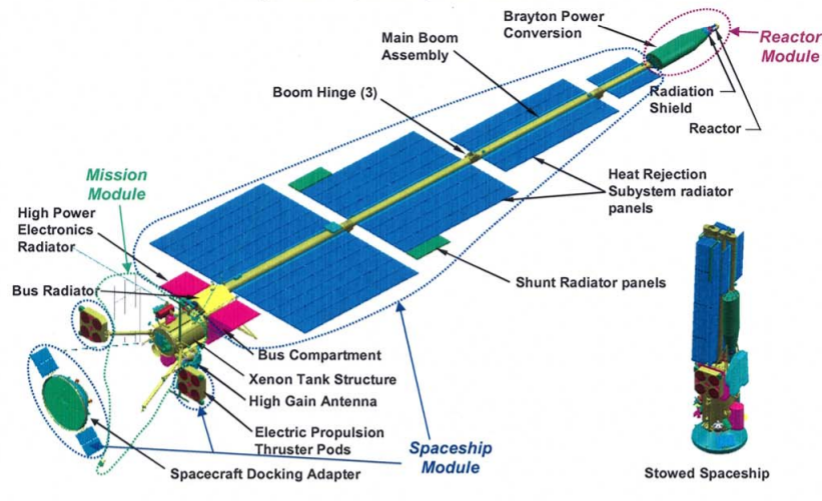
\includegraphics[height=0.45\textheight]{fig/appS}
	\caption[Jupiter Icy Moon Spaceship]{Jupiter Icy Moon Spaceship~\cite{edwards2012overview}}
	\label{appS}
\end{figure}

Since Project Prometheus only operated for a few years, many of these systems were not completed, and there is only information of what was tested. The types of reactors being tested were liquid metal, heatpipe, and gas cooled reactors~\cite{wollman2006prometheus}. The possible coolants were liquid alkali metals like Li, non-alkaala metals like Pb-Bi, molten salts like F, and gas like He-Xe~\cite{wollman2006prometheus}. The fuel material was planned to be UO2, UN, or UC/UC2 in fuel pellets similar to TRISO or in ceramic or metallic spheres~\cite{wollman2006prometheus}. Cladding and core would be refractory metal alloys like Nb or Re, conventional metal alloys like stainless steel, and SiC ceramics~\cite{wollman2006prometheus}. The power conversion was a Brayton type and two main types were investigated: super alloys in inert gases and IN-792, Hast-X, IN-617, and MA956 in air~\cite{taylor2005prometheus}. Heatpipes were planned for heat rejection, using water heatpipes, high temperature organic, and ceramic materials~\cite{taylor2005prometheus}. Heat rejection would use coolants such as NaK, water, or Li~\cite{wollman2006prometheus}.


The electric propulsion systems were completed, showing that either NEXIS or HiPEP could give the required specific impulse of 6,000 to 9,000 seconds, have an efficiency greater than 65\%, and had power levels of 20 to 40 kW~\cite{taylor2005prometheus}. The high power telecommunicators were to be two 180W Ka-Band Traveling Wave Tubes or a 250W Traveling Wave Tube~\cite{taylor2005prometheus}. Progress was made in finding radiation hardened electronics/parts, completing the Honeywell Rad Hard ASIC fabrication line, the Rad Hard ASICs for IEEE 1394A and 12C data bases, the Rad Hard power control mixed signals ASICs, and the RAD750 processor development~\cite{taylor2005prometheus}. On top of this, radiation models for valves and pressure transducers for the propellent management were completed~\cite{taylor2005prometheus}. For low thrust trajectory tools, dynamic prototype software tools were designed~\cite{taylor2005prometheus}.


Several shielding configurations and materials were tried, including an Al/Ta shield material which was found to give the same properties as pure Al with 10\% less mass. The other materials used were the usual BeO, B4C, LiH~\cite{wollman2006prometheus}. The initial shield mass was estimated to be 1500 kg for the final design, but was expected to decrease as models and configurations were developed~\cite{taylor2005prometheus}. A full list of materials considered with developmental concerns is available in Figure~\ref{appT} with the pros and cons of fuel materials listed in Figure~\ref{appU}. 


\begin{figure}[]
	\centering
	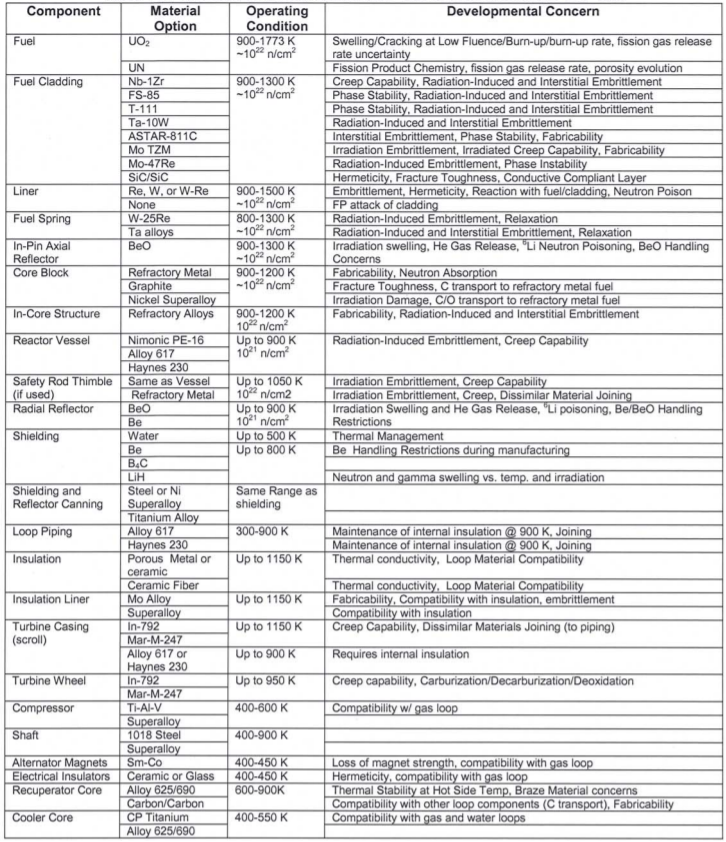
\includegraphics[height=0.85\textheight]{fig/appT}
	\caption[JIMO Materials and Developmental Concerns]{JIMO Materials and Developmental Concerns~\cite{wollman2006prometheus}}
	\label{appT}
\end{figure}

\begin{figure}[]
	\centering
	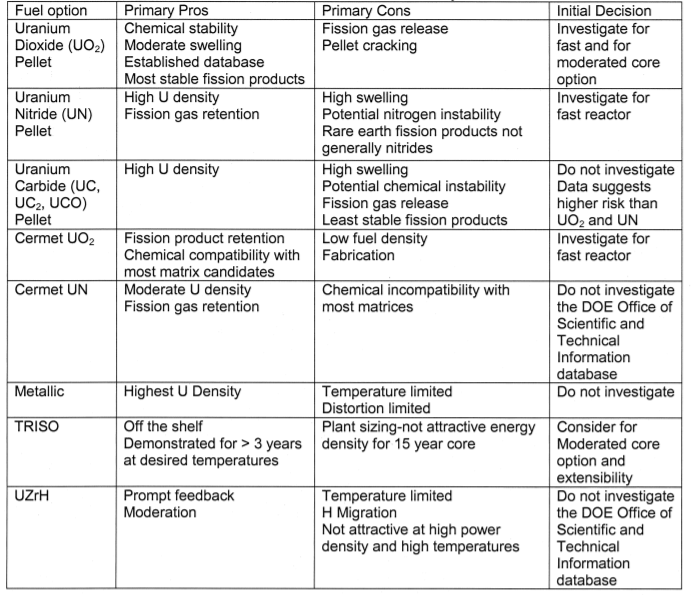
\includegraphics[height=0.45\textheight]{fig/appU}
	\caption[Pros and Cons of Fuel Types considered on the JIMO]{Pros and Cons of Fuel Types considered on the JIMO~\cite{wollman2006prometheus}}
	\label{appU}
\end{figure}






\section{Propulsion Systems}

When discussing rocket science, a fundamental measure of performance is that of specific impulse, which roughly speaking is the amount of thrust you get per unit mass flow of fuel and is in units of inverse seconds. One equation used to describe impulse is :

\begin{equation}
\label{eq1}
I_{sp} = A*C_f*\left(\frac{T_c}{M}\right)^{\frac{1}{2}}
\end{equation}

where $A$ is a thermophysical of the property of the propellant, $C_f$ is the thrust coefficient and is a function of nozzle parameters, $T_c$ is the temperature of the chamber, and $M$ is the molecular weight of the exhaust gases~\cite{buden2011space}. Nuclear powered rockets have an edge over other conventional rocket designs because of the high chambers emperatures they can reach, and without combusting hydrogen, thereby increasing the specific impulse of the exhaust compared to conventional rockets. Typical conventional rockets have impulses in the realm of 400-500 $s$~\cite{buden2011space}. Nuclear rockets, through several research initiatives, proved to have specific impulses on the order of 1000 $s$~\cite{matthews1993fuels}. A high specific impulse allows a vehicle to reach higher speeds with the same amount of fuel. With missions concerning distant objects such as the oort cloud, many missions are prohibited simply by the timescale involved. With high specific impulses, even standard maneuvers offer much shorter time commitments for missions, and missions to the very edge of the solar system become possible. Based off of many parameters from the New Horizons mission, it is within the realm of possibility to reach the Oort cloud within five or six years.


From Equation~\ref{eq1}, one may see that the specific impulse may be maximized by having as high of temperatures as possible, while have the lowest molecular weight as possible~\cite{specimp}. The gas with the lowest molecular weight is hydrogen, which is already used in most rockets. In terms of nuclear reactor physics, this is a benefit since hydrogen is an excellent thermalizing medium for neutrons. However, two problems arise from using hydrogen. The first is that many of the early designs for nuclear rockets involved the use of graphite, which was the primary moderator~\cite{matthews1993fuels}. When hydrogen is put in contact with carbon based materials at high temperatures, hydrocarbon gases are produced which impedes on the specific impulse due to the higher molecular weight of the exhaust. Second, is that the high temperature of the chamber involves operating at the very edge of the material constraints. In other words, the high temperature performance results in a much lower reactor lifetime~\cite{lyon1973performance}. Despite these two design hurdles, the early nuclear rocket programs were able to produce design of specific impulses of about 1000 $s$, and the NERVA program was able to produce a design capable of 10 hours of run time~\cite{buden2011space}.

A typical nuclear propulsion module is displayed in Figure~\ref{appAA}.

\begin{figure}[]
	\centering
	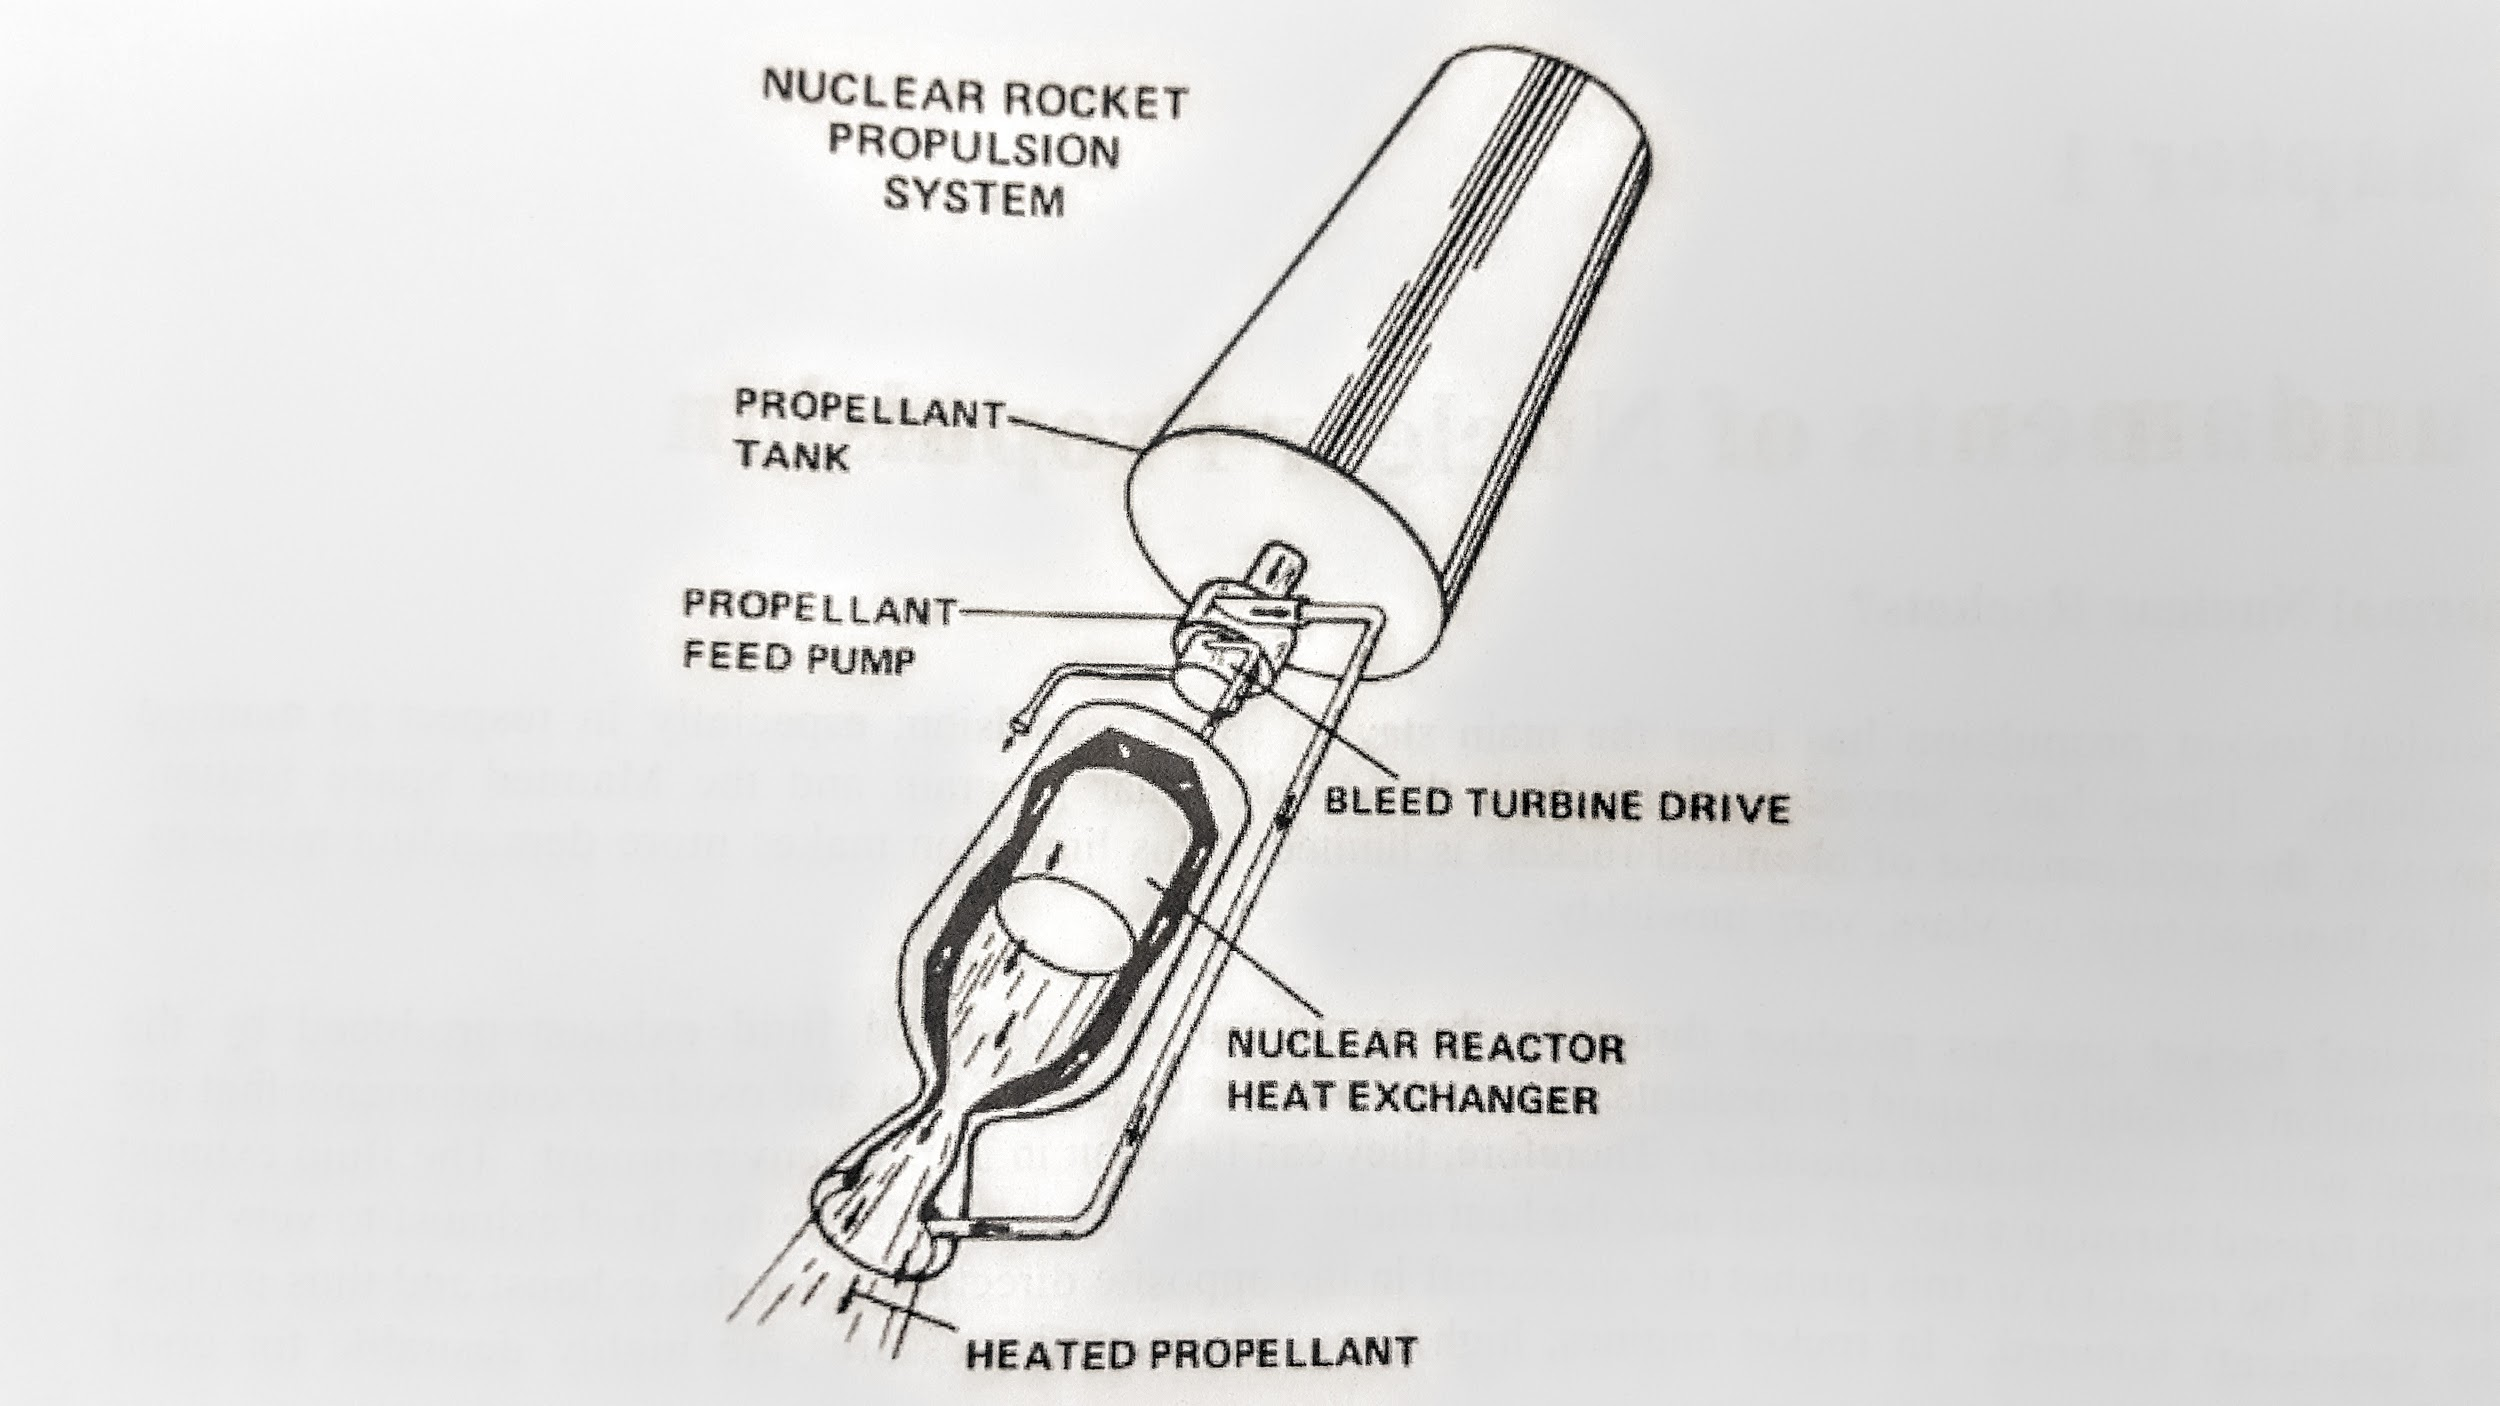
\includegraphics[height=0.45\textheight]{fig/appAA}
	\caption[Typical Nuclear Propulsion Module]{Typical Nuclear Propulsion Module~\cite{taub1975review}}
	\label{appAA}
\end{figure}

One difference between these missions and this project is that the earlier programs all operated on very high enriched uranium fuel assemblies (~93\% U-235), whereas this project calls for low-enriched uranium. This means that many of the key design concepts from the missions that are known cannot be used. Many geometric aspects will change, such as diameter, length size of fuel rods, which will in turn aggravate known issues in existing reactors both in nuclear rocket designs and conventional reactors. For instance, there may be larger temperature gradients, less distributed reactivity may cause the reactor be more temperamental to perturbations etc.


A mission to the Oort cloud, fortunately, does not require a large thrust for a short time. A smaller thrust over a longer period of time may yield the same results. This however may require special attention to erosion to the core. One specific issue with earlier missions was that of “mid-range corrosion.” In these reactors, hydrogen flowed from top to bottom, with the hydrogen gas entering at a relatively low temperature, heating, and exiting through the bottom of the core. In the middle of the reactor, because of the high neutron flux and the hydrogen being most of the way heated, the fuel suffered particularly large corrosion in the middle-range of the reactor~\cite{raj2015development}. This effect limits the highest temperatures to be in the center of the core, which will lower the heat transfer to the hydrogen. One workaround for this effect was the use of the thruster cone as a pre-heater. That is, before going through the core, the hydrogen was pumped through a portion of the thruster skirt. This not only cooled the skirt which increased liability, but it also allowed the hydrogen entering the core to receive more heat from the reactor core, and lowered the temperature gradient through the core.


Much of the testing involved in the earlier programs involved analysis of different material choices for the fuel and coolant channels in order to counter the corrosion of the core over time. Carbide fuels were found to be the most reliable, and various amounts of ZrC were added to test strength as a coating or mixed with the Uranium Carbide and graphite in a composite~\cite{lyon1973performance}. Much of the design process will rely heavily on the experimental results from these and other tests, since the ability to test materials in-house is severely limited. The most favorable combination found was a carbide fuel with ZrC coating when operating at 3000 K which produced a theoretical specific impulse of near 1200 s-1, however all material choices performed identically near 2000 K with a specific impulse of approximately 750 s-1. A more in-depth astro mechanical analysis will need to be performed to determine what minimum specific impulse will be required.
Another design constraint was the ability of the engine to restart. As a mechanical requirement, the reactor will have to be periodically cooled to remove the decay heat from the reactor. The decay heat produces thermal power proportional to the power the reactor was running at. After the engine has run through it's primary burn, and if it is expected to be used again, hydrogen will have to pump through the core to cool it off in order to protect reactor components. Additionally, the speed may be increased with less propellant by performing perigee maneuvers. In a perigee maneuver, a vehicle uses the Earth as a gravity assist one or more time before the vehicle finally leaves orbit~\cite{rom1991review}. A perigee maneuver, depending on the number of passes, may drastically lower the amount of power needed by the reactor, which in turn lowers the decay heat, which lowers the number of restarts. In the NERVA and ROVER programs, a secondary mode was planned in which the reactor operated at 1MWt for this purpose~\cite{booth1975}.


Since the NERVA and ROVER programs, fast-neutron reactor designs that have come out using UN fuel as opposed to UC fuel. For instance, the SCoRe reactor from the University of New Mexico is a fast reactor design that  utilizes UN fuel with a BeO reflector. The reactor is made to operate on the fast spectrum, so that in the event of a failed launch and the reactor is submerged, the reactor will not go critical~\cite{hatton2009sectored}. This is partially done by the use of spectral shift absorbers, which are thermal neutron absorbers that leech thermal neutrons. One downside to design such as these are that the reactors, in and of themselves, are not bimodal. That is, a robust power conversion system would be required to produce electricity for a propulsion system.


Other reactors, notably the Safe Affordable Fission Engine (SAFE) and the Heatpipe Operated Mars Exploration Reactor (HOMER) were researched and showed promising design specifications. They were both considered reliable power systems with a range of power production levels~\cite{poston2001heatpipe,van2002testing}. They too, however, were only made to produce electricity and not direct thrust. The SCoRe, SAFE, and HOMER reactors were also never tested, whereas the thermal rocket programs from the Apollo era were tested extensively and have reliable data. Going forward, a decision will have to be made as to whether the Oort Cloud explorer will have a reactor that offers direct thrust, or a more robust electric conversion system for a secondary thrust system. With the direct thrust, designs based off of NERVA, Phoebus, and Kiwi reactors will have a high confidence in overall performance, because they were proven nearly up to flight readiness~\cite{buden2011space}. If the project follows the line of the the SCoRe, Safe, and HOMER reactors then much of the design will rely on the theoretical performance that was left unproven.



\begin{figure}[H]
	\centering
	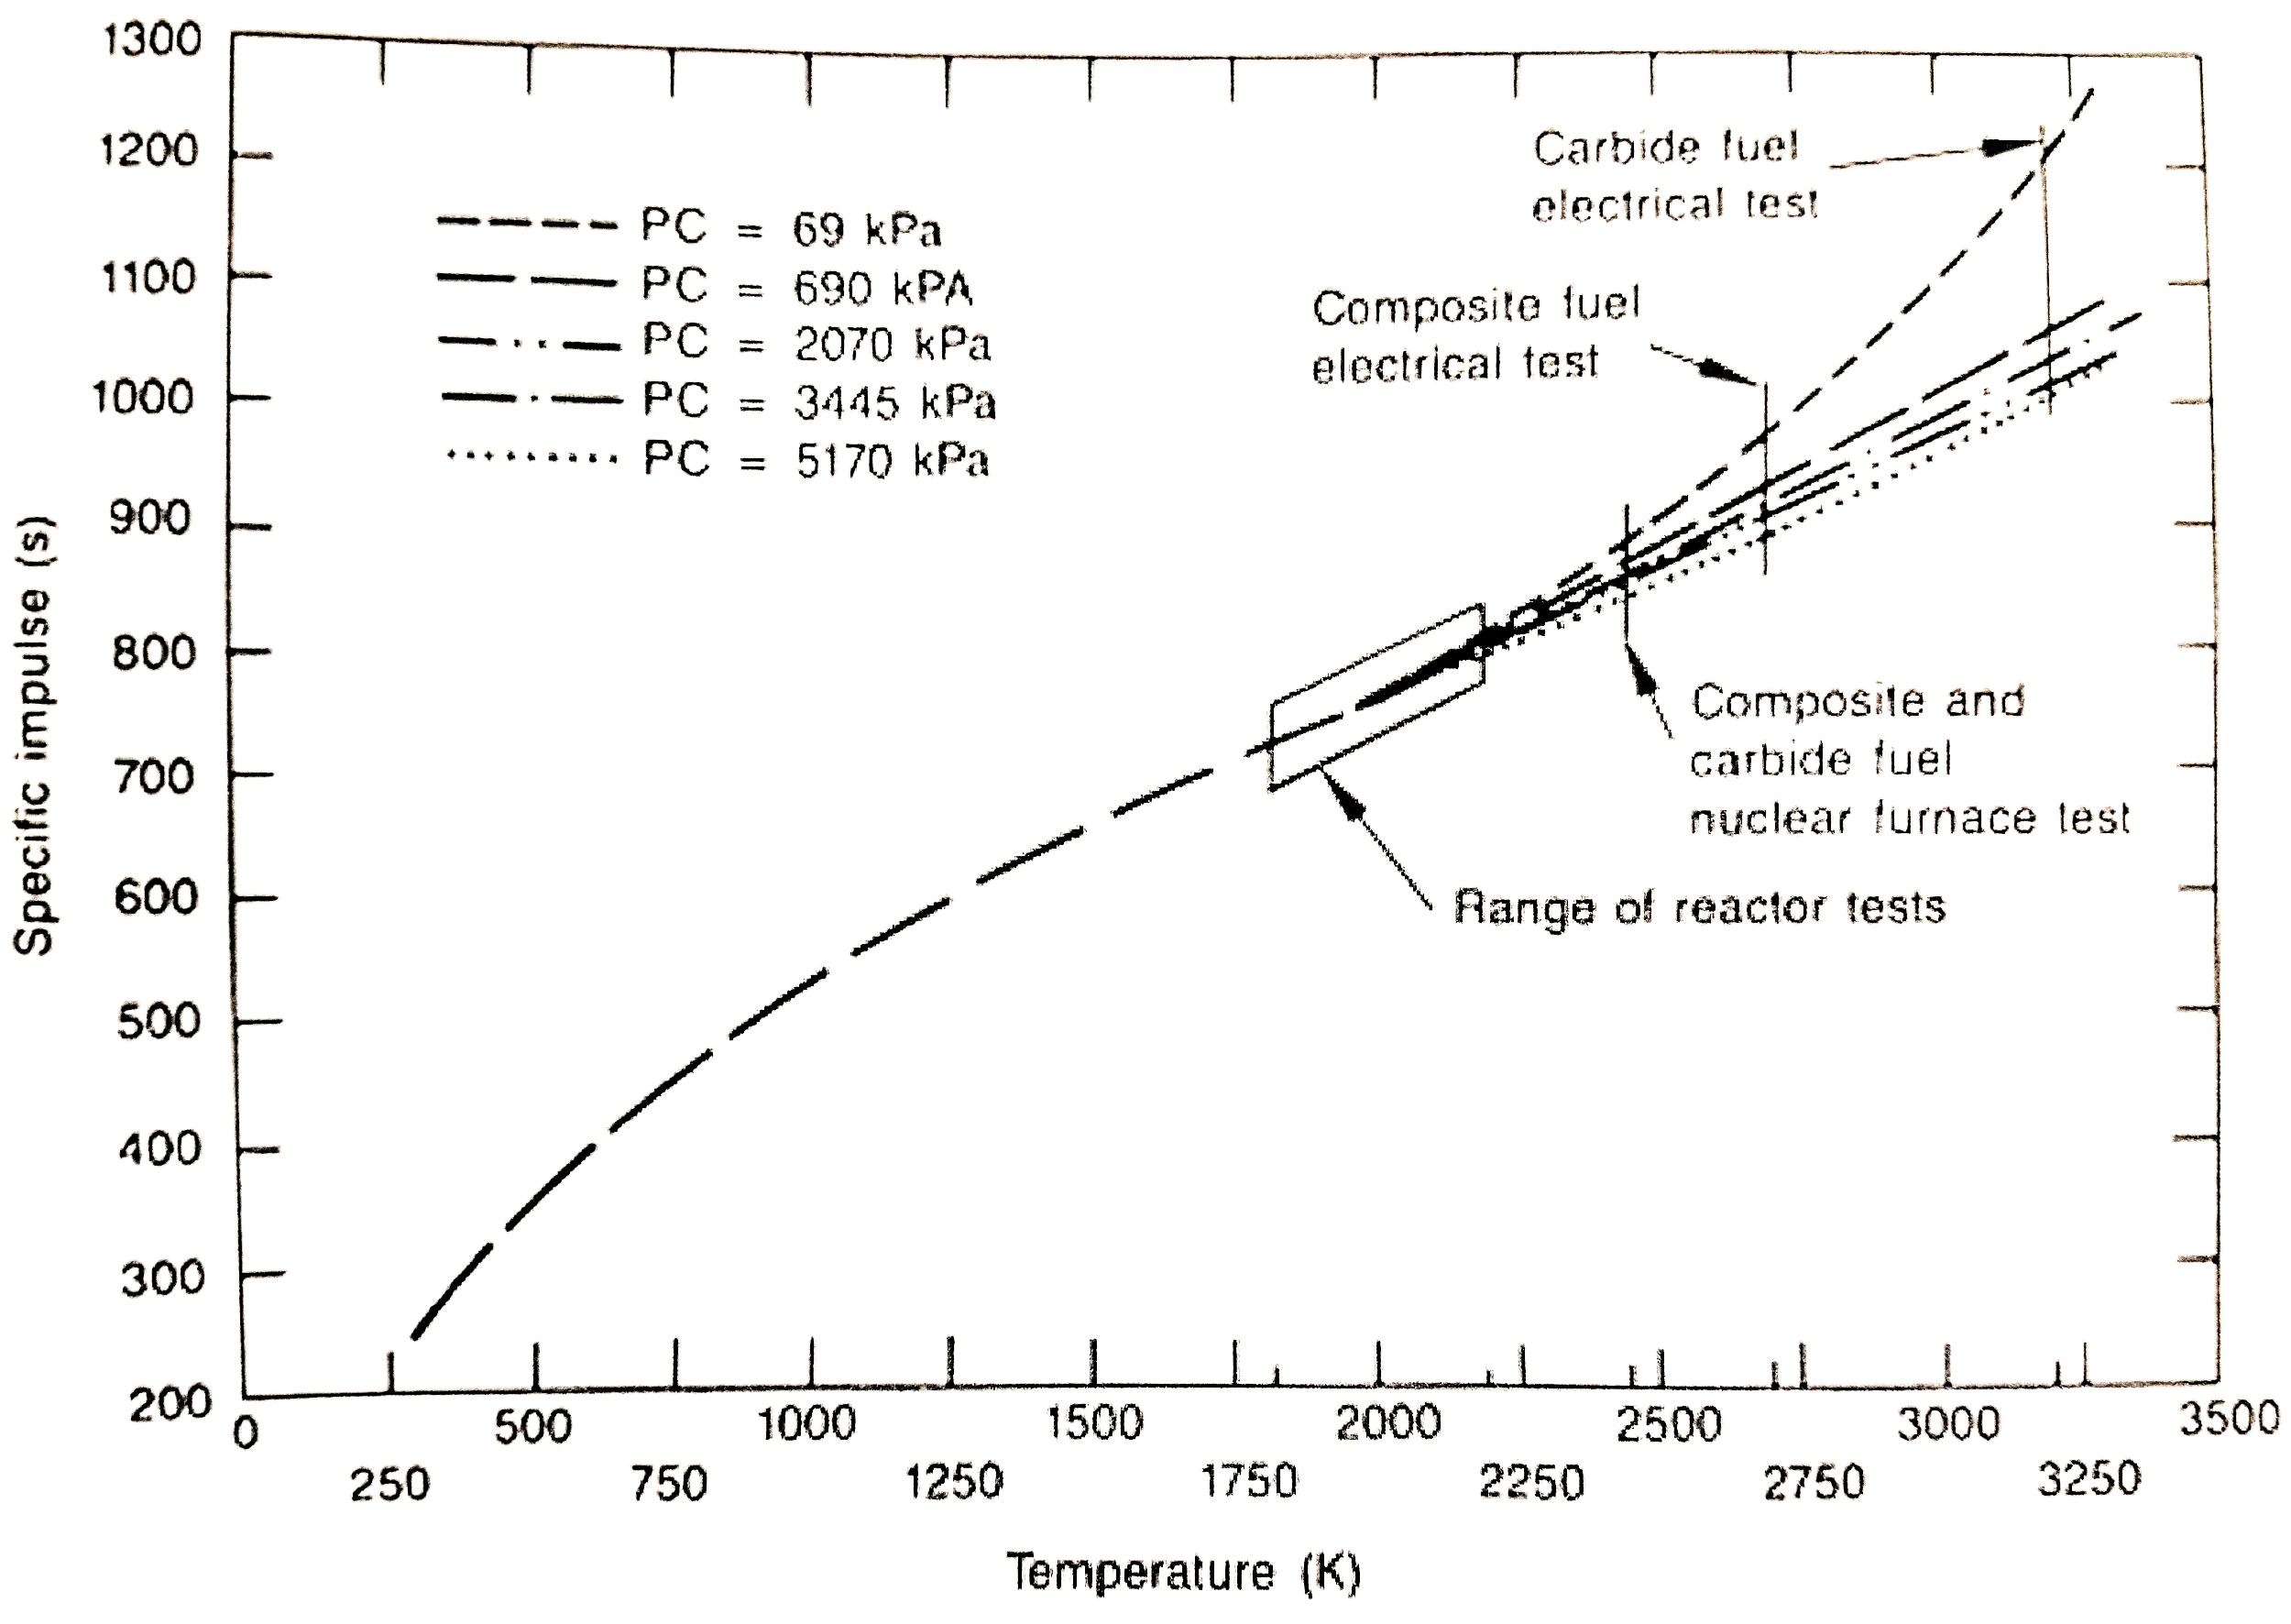
\includegraphics[height=0.45\textheight]{fig/appW}
	\caption[Specific impulse versus exhaust nozzle temperature for nozzle area ratio 300]{Specific impulse versus exhaust nozzle temperature for nozzle area ratio 300~\cite{buden1970operational}}
	\label{appW}
\end{figure}


\begin{figure}[H]
	\centering
	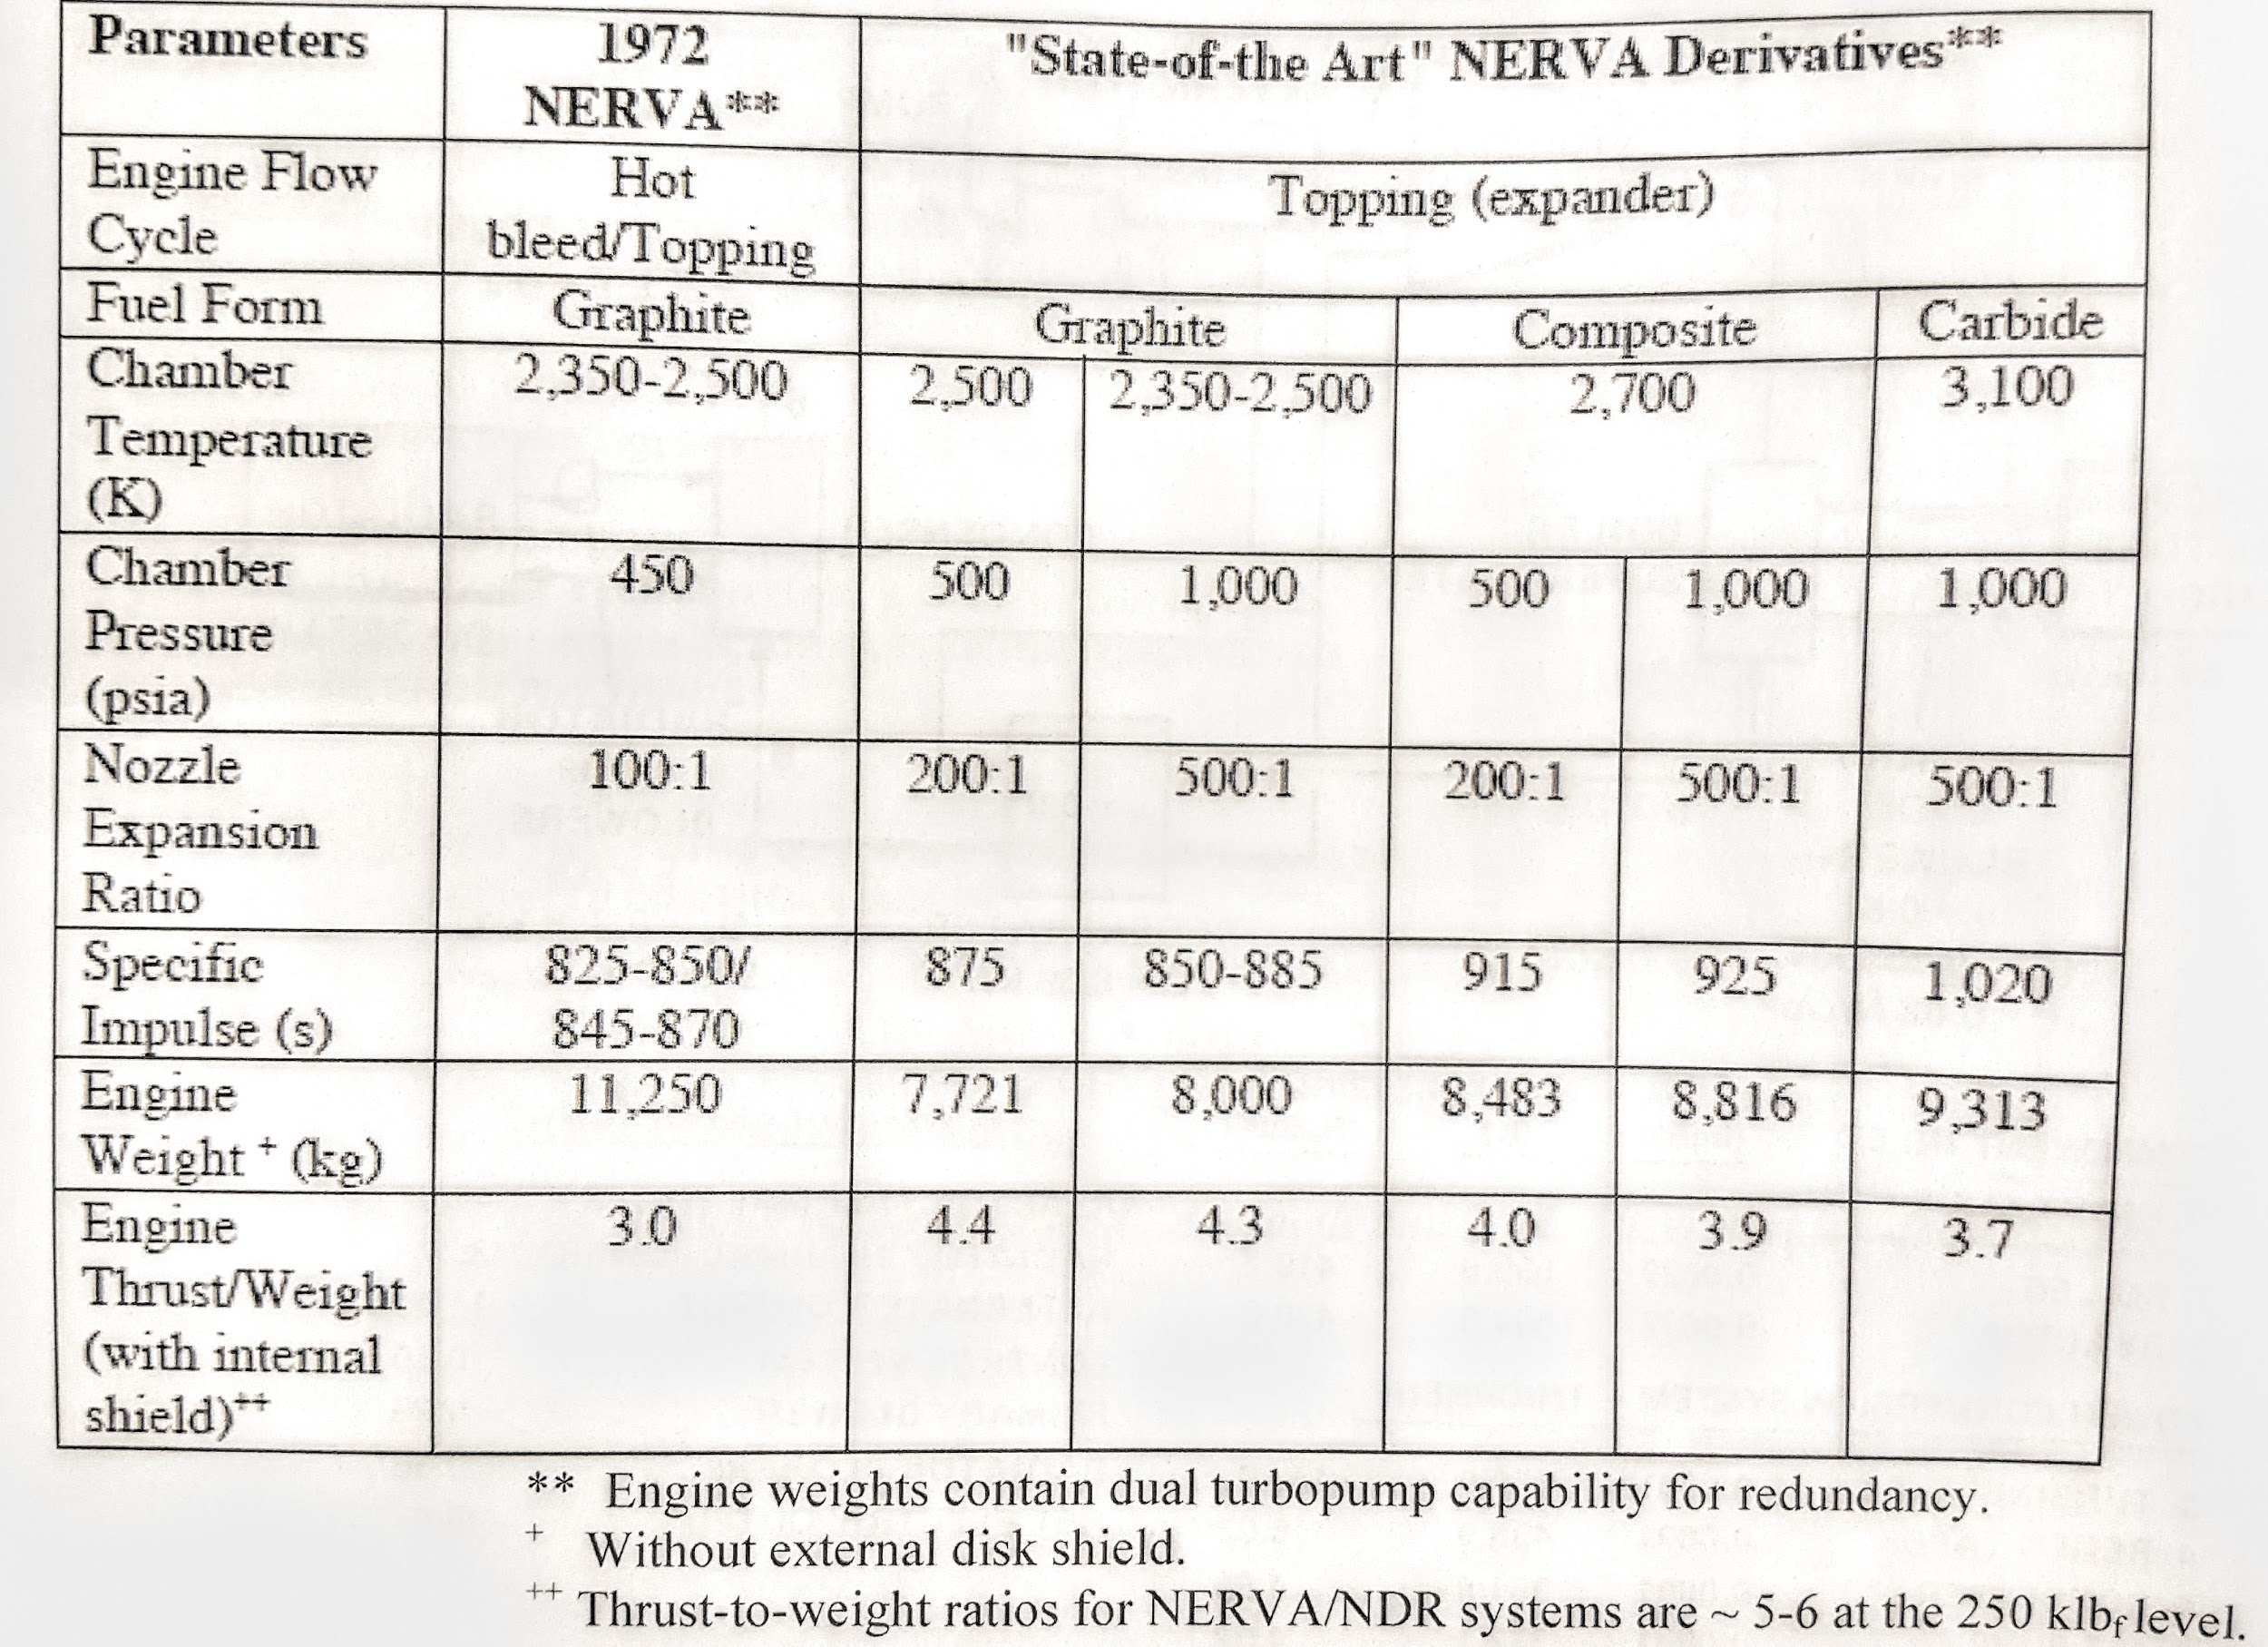
\includegraphics[height=0.45\textheight]{fig/appY}
	\caption[Characteristics for 337 kN (75,000 lbf) NERVA type engines]{Characteristics for 337 kN (75,000 lbf) NERVA type engines~\cite{borowski1994rationale}}
	\label{appY}
\end{figure}


\begin{figure}[H]
	\centering
	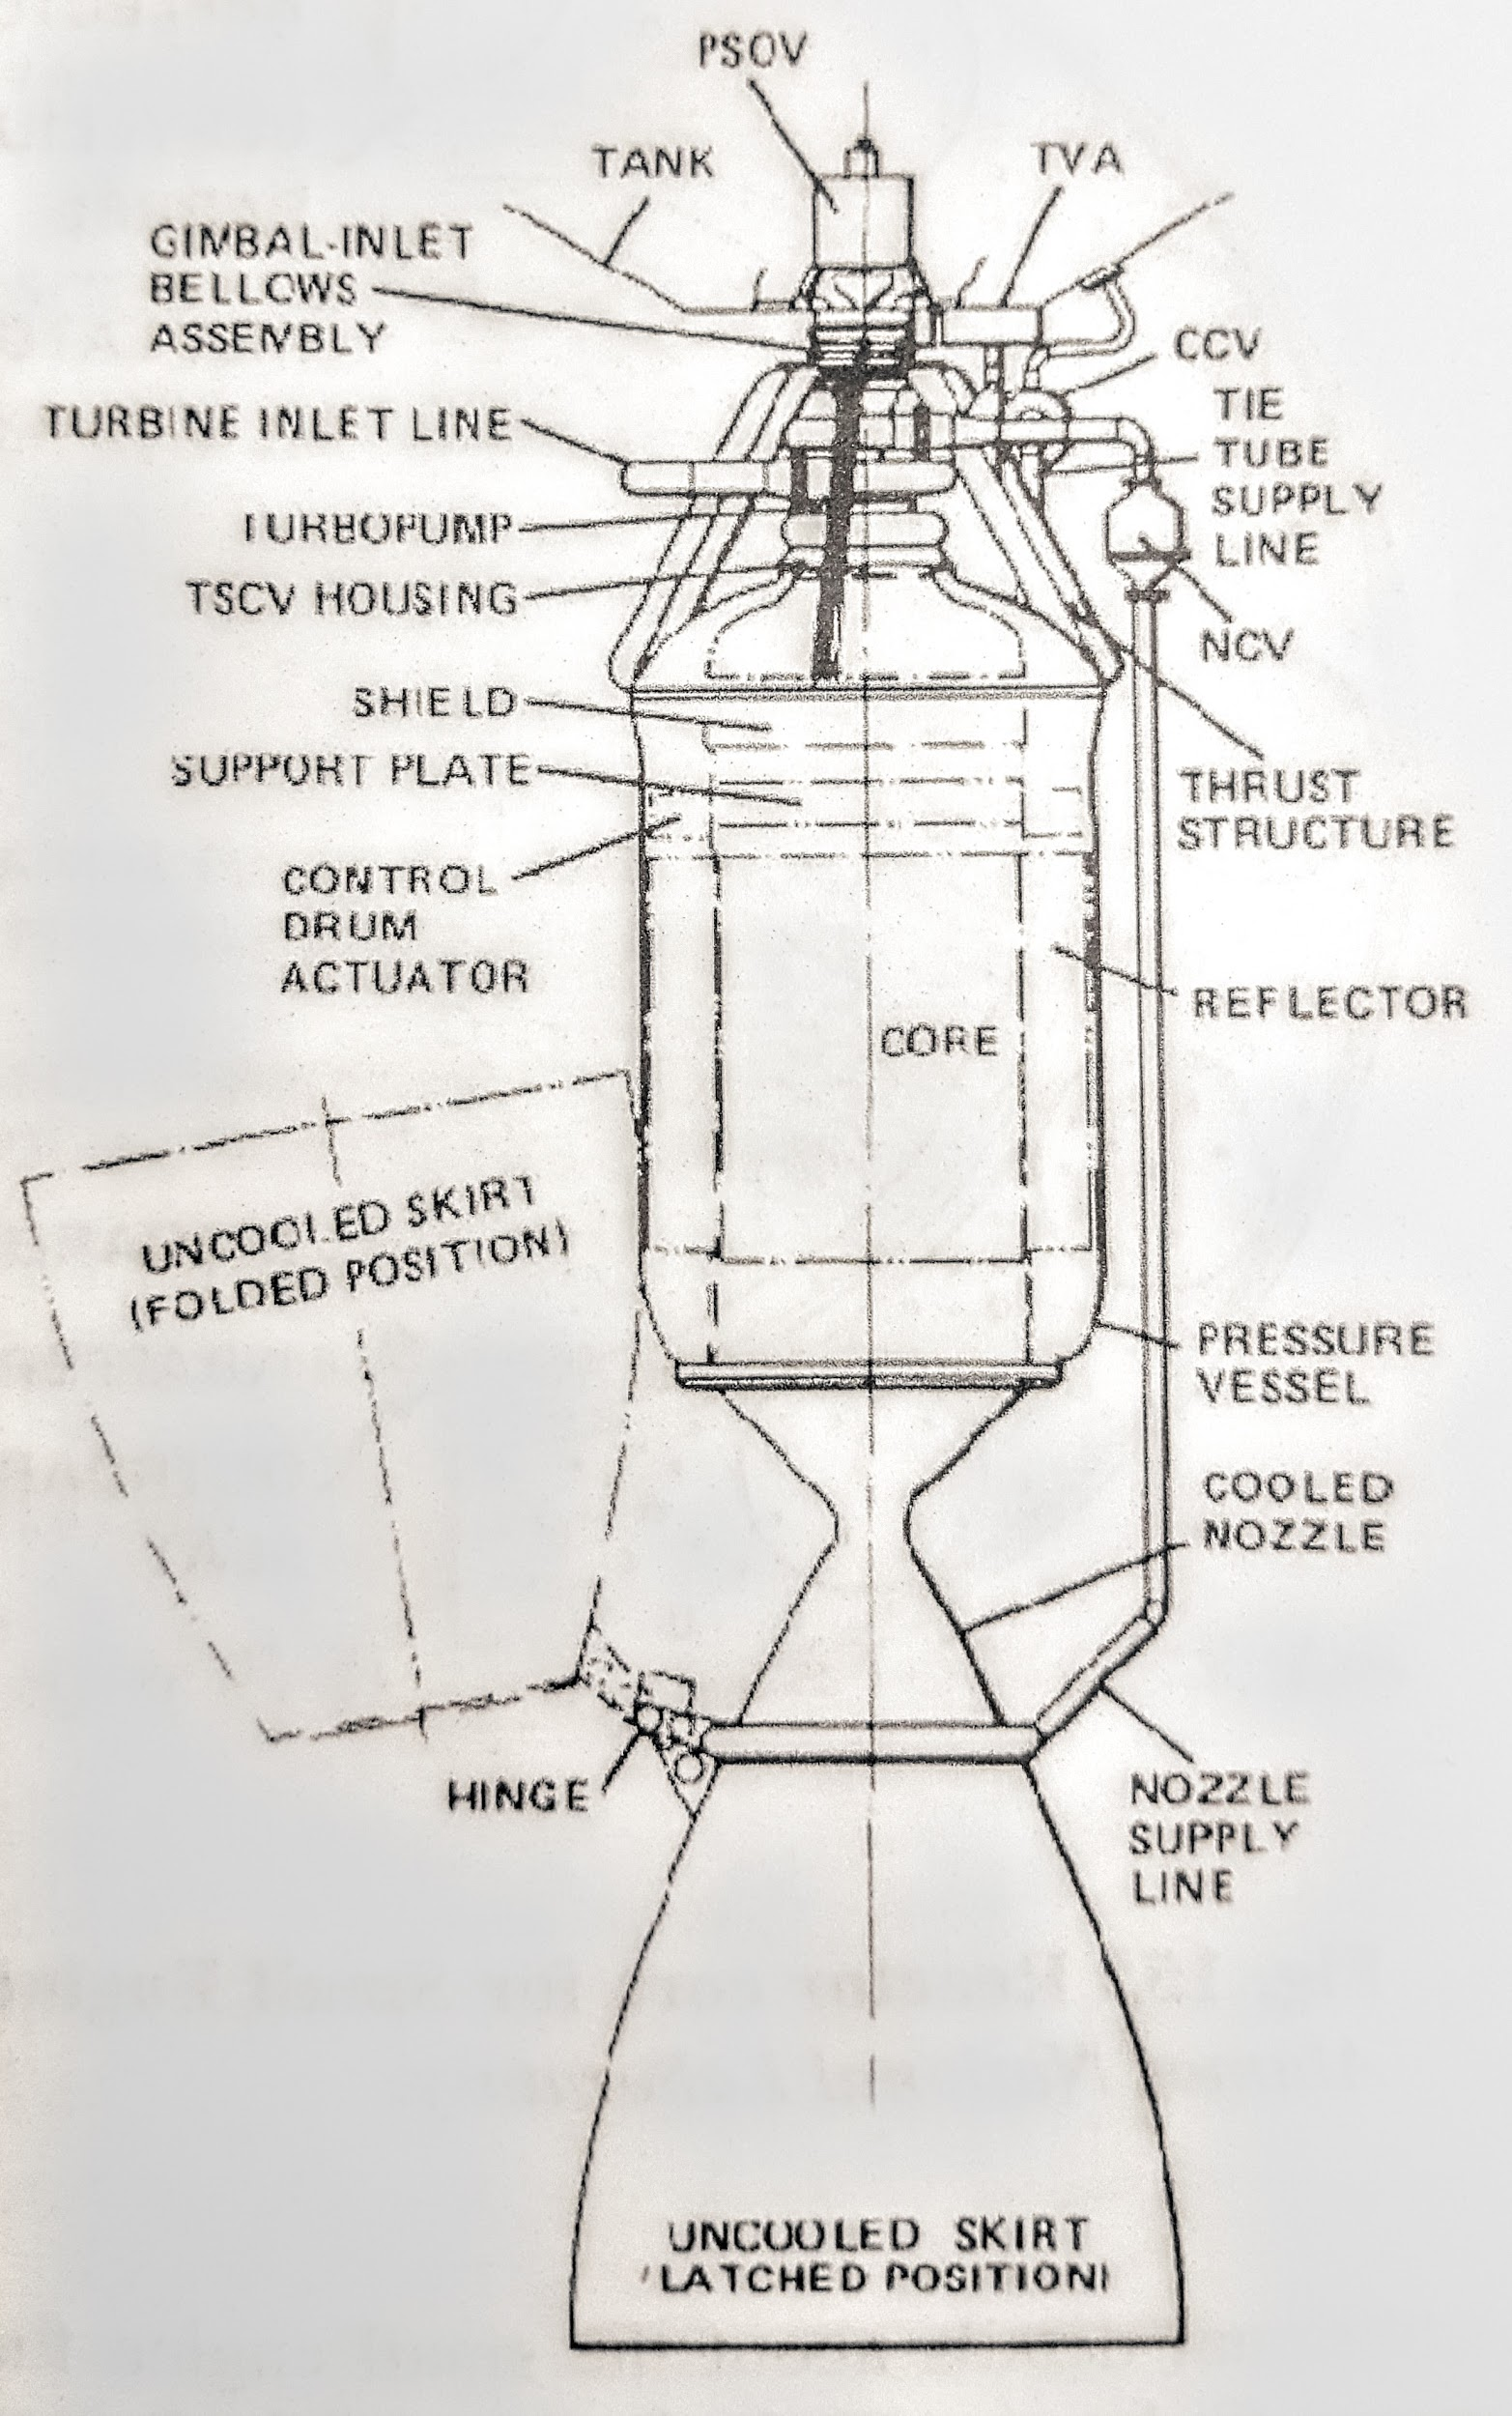
\includegraphics[height=0.45\textheight]{fig/appZ}
	\caption[Small Engine Nuclear Rocket design schematic]{Small Engine Nuclear Rocket design schematic~\cite{durham1972nuclear}}
	\label{appZ}
\end{figure}



\section{Electrical Systems}

\subsection{Early Generations of Thermoelectric Generators}

Currently, all US space missions have employed a thermoelectric (TE) conversion system for space missions. They have the distinct advantage of containing no moving parts, allowing them to be high reliable. However, they generally suffer from low efficiencies, around 10\%. Thermoelectric power systems take advantage of the Seebeck effect, a phenomenon where two dissimilar metals at different temperatures induces an electromotive force, causing a current to appear. Ideal thermoelectric generators have a high Seebeck coefficient, low thermal conductivity to ensure a high temperature gradient, and high electric conductivity. Low resistivity also allows systems to become more efficient.~\cite{buden1979selection}

	Several thermoelectric power systems have been employed, and can be split into their semiconductor materials~\cite{anderson1983space}. Systems that have utilized Tellurides include Transit Navigation Satellites (SNAP-3A, SNAP-9A), the Nimbus III Meteorological Satellite (SNAP-19B), and the Pioneer 10 and 11 flybys of Jupiter, Saturn, and beyond (SNAP-19). Further Telluride TE systems were present on the Viking Mars Lander (SNAP-19), the Apollo Lunar Landings (SNAP-27), and may be used on the Mars Science Laboratory Rover (MRTG), as seen in Tables~\ref{table1} and~\ref{table2}. 

	TE systems were also available with a semiconductor made of Silicon Germanium. Several missions were made possible through this technology, including the Lincoln Experimental Satellites 8/9 (Multihundred Watt Generator-MHW), Voyager 1 and 2 (MHW), the SNAP-10A U-ZrH Experimental Nuclear Reactor in Earth Orbit, the Galileo Jupiter Orbiter (GPHS-RTG), the Ulysses Planetary/Solar Exploration (GPHS-RTG), the Cassini Orbiter to Saturn, and New Horizons (GPHS-RTG)~\cite{dassoulas2007rtgs}.

	TE systems must employ a heat rejection subsystem to get rid of waste heat. Radiators are designed to vent the excess heat to space, and their design depends on the amount of heat to be ejected and the operating temperature of the system. For most TE power systems, operating temperatures are around 575K, due to the amount of heat that may be directly radiated to space. This is dependent on the Stefan-Boltzmann law, and states that the heat that can be radiated is proportional to the fourth power of the radiator surface area.


\begin{figure}[]
	\centering
	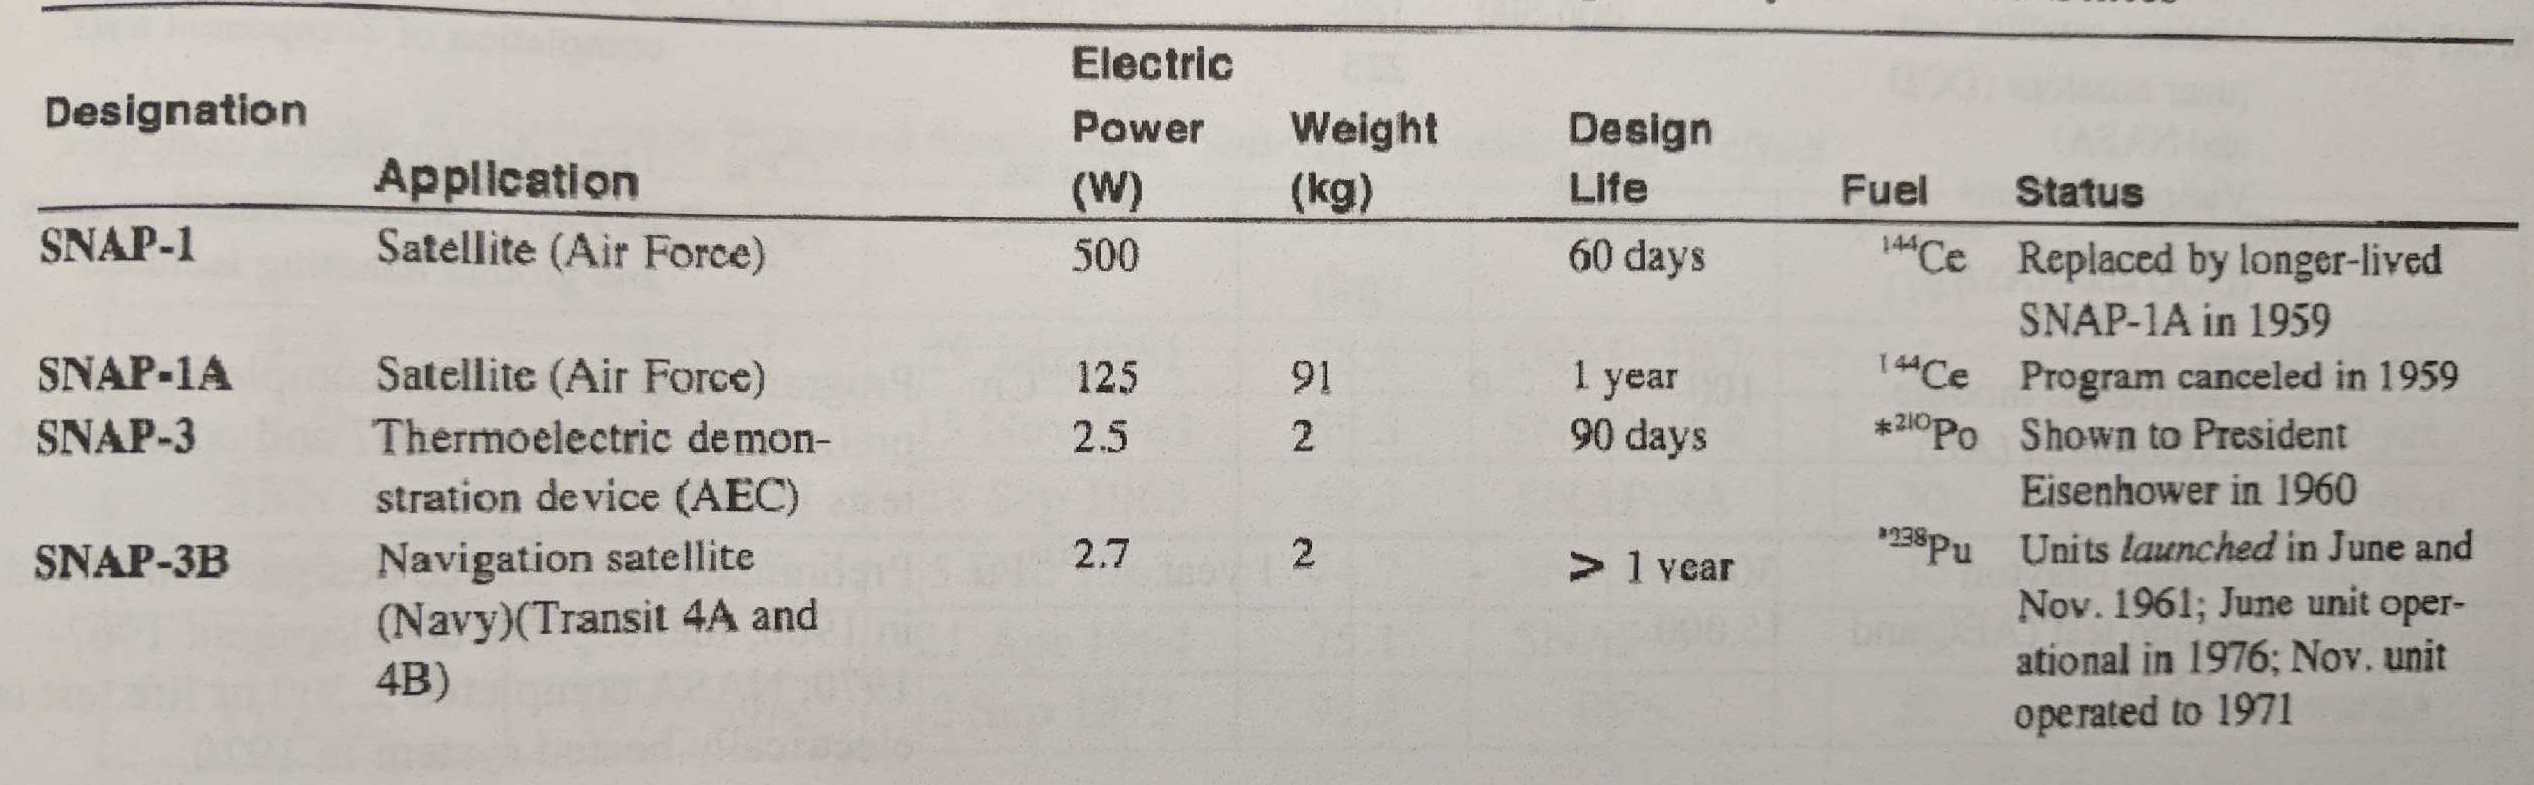
\includegraphics[height=0.20\textheight]{fig/table1}
	\caption[Radioisotope Generators Developed for Space Electric Power by the USA]{Radioisotope Generators Developed for Space Electric Power by the USA~\cite{buden2011spacebook1}}
	\label{table1}
\end{figure}

\begin{figure}[]
	\centering
	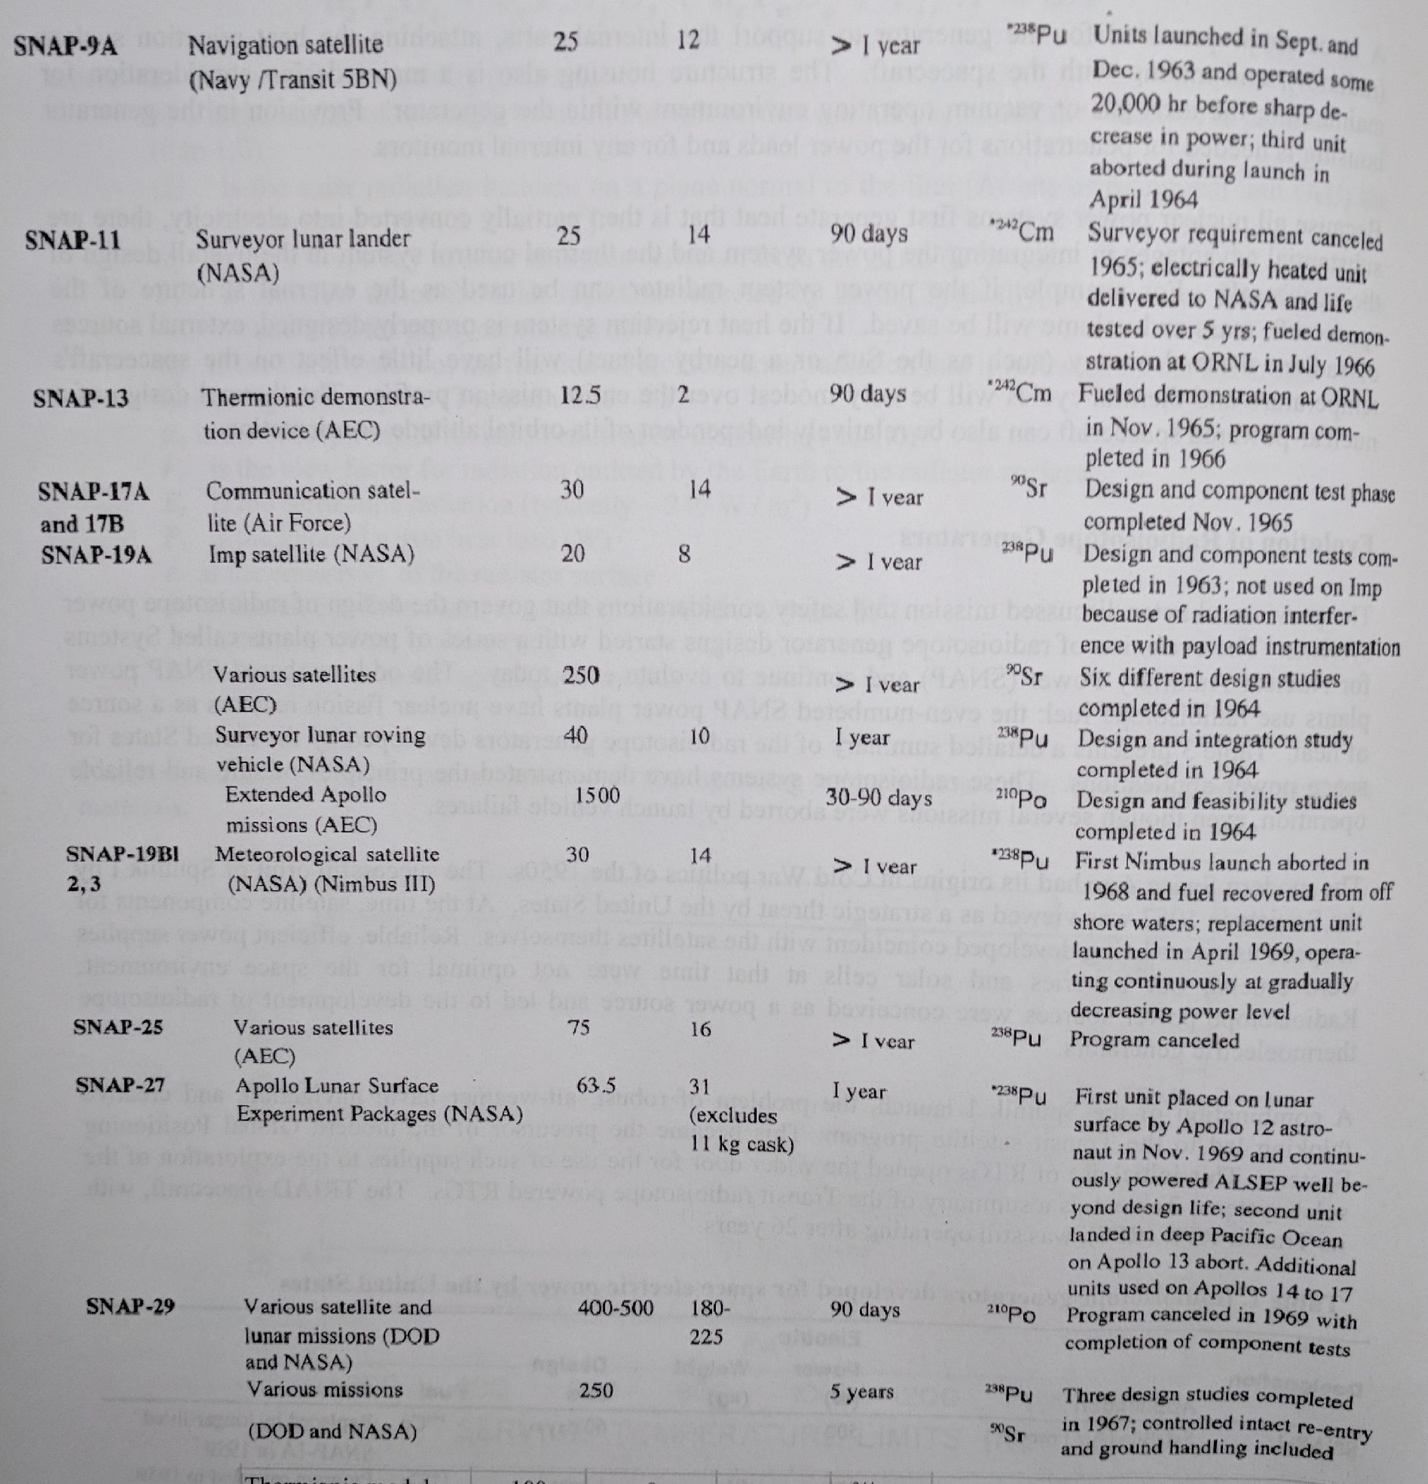
\includegraphics[height=0.55\textheight]{fig/table2}
	\caption[Radioisotope Generators Developed for Space Electric Power by the USA]{Radioisotope Generators Developed for Space Electric Power by the USA~\cite{buden2011spacebook1}}
	\label{table2}
\end{figure}

\begin{figure}[]
	\centering
	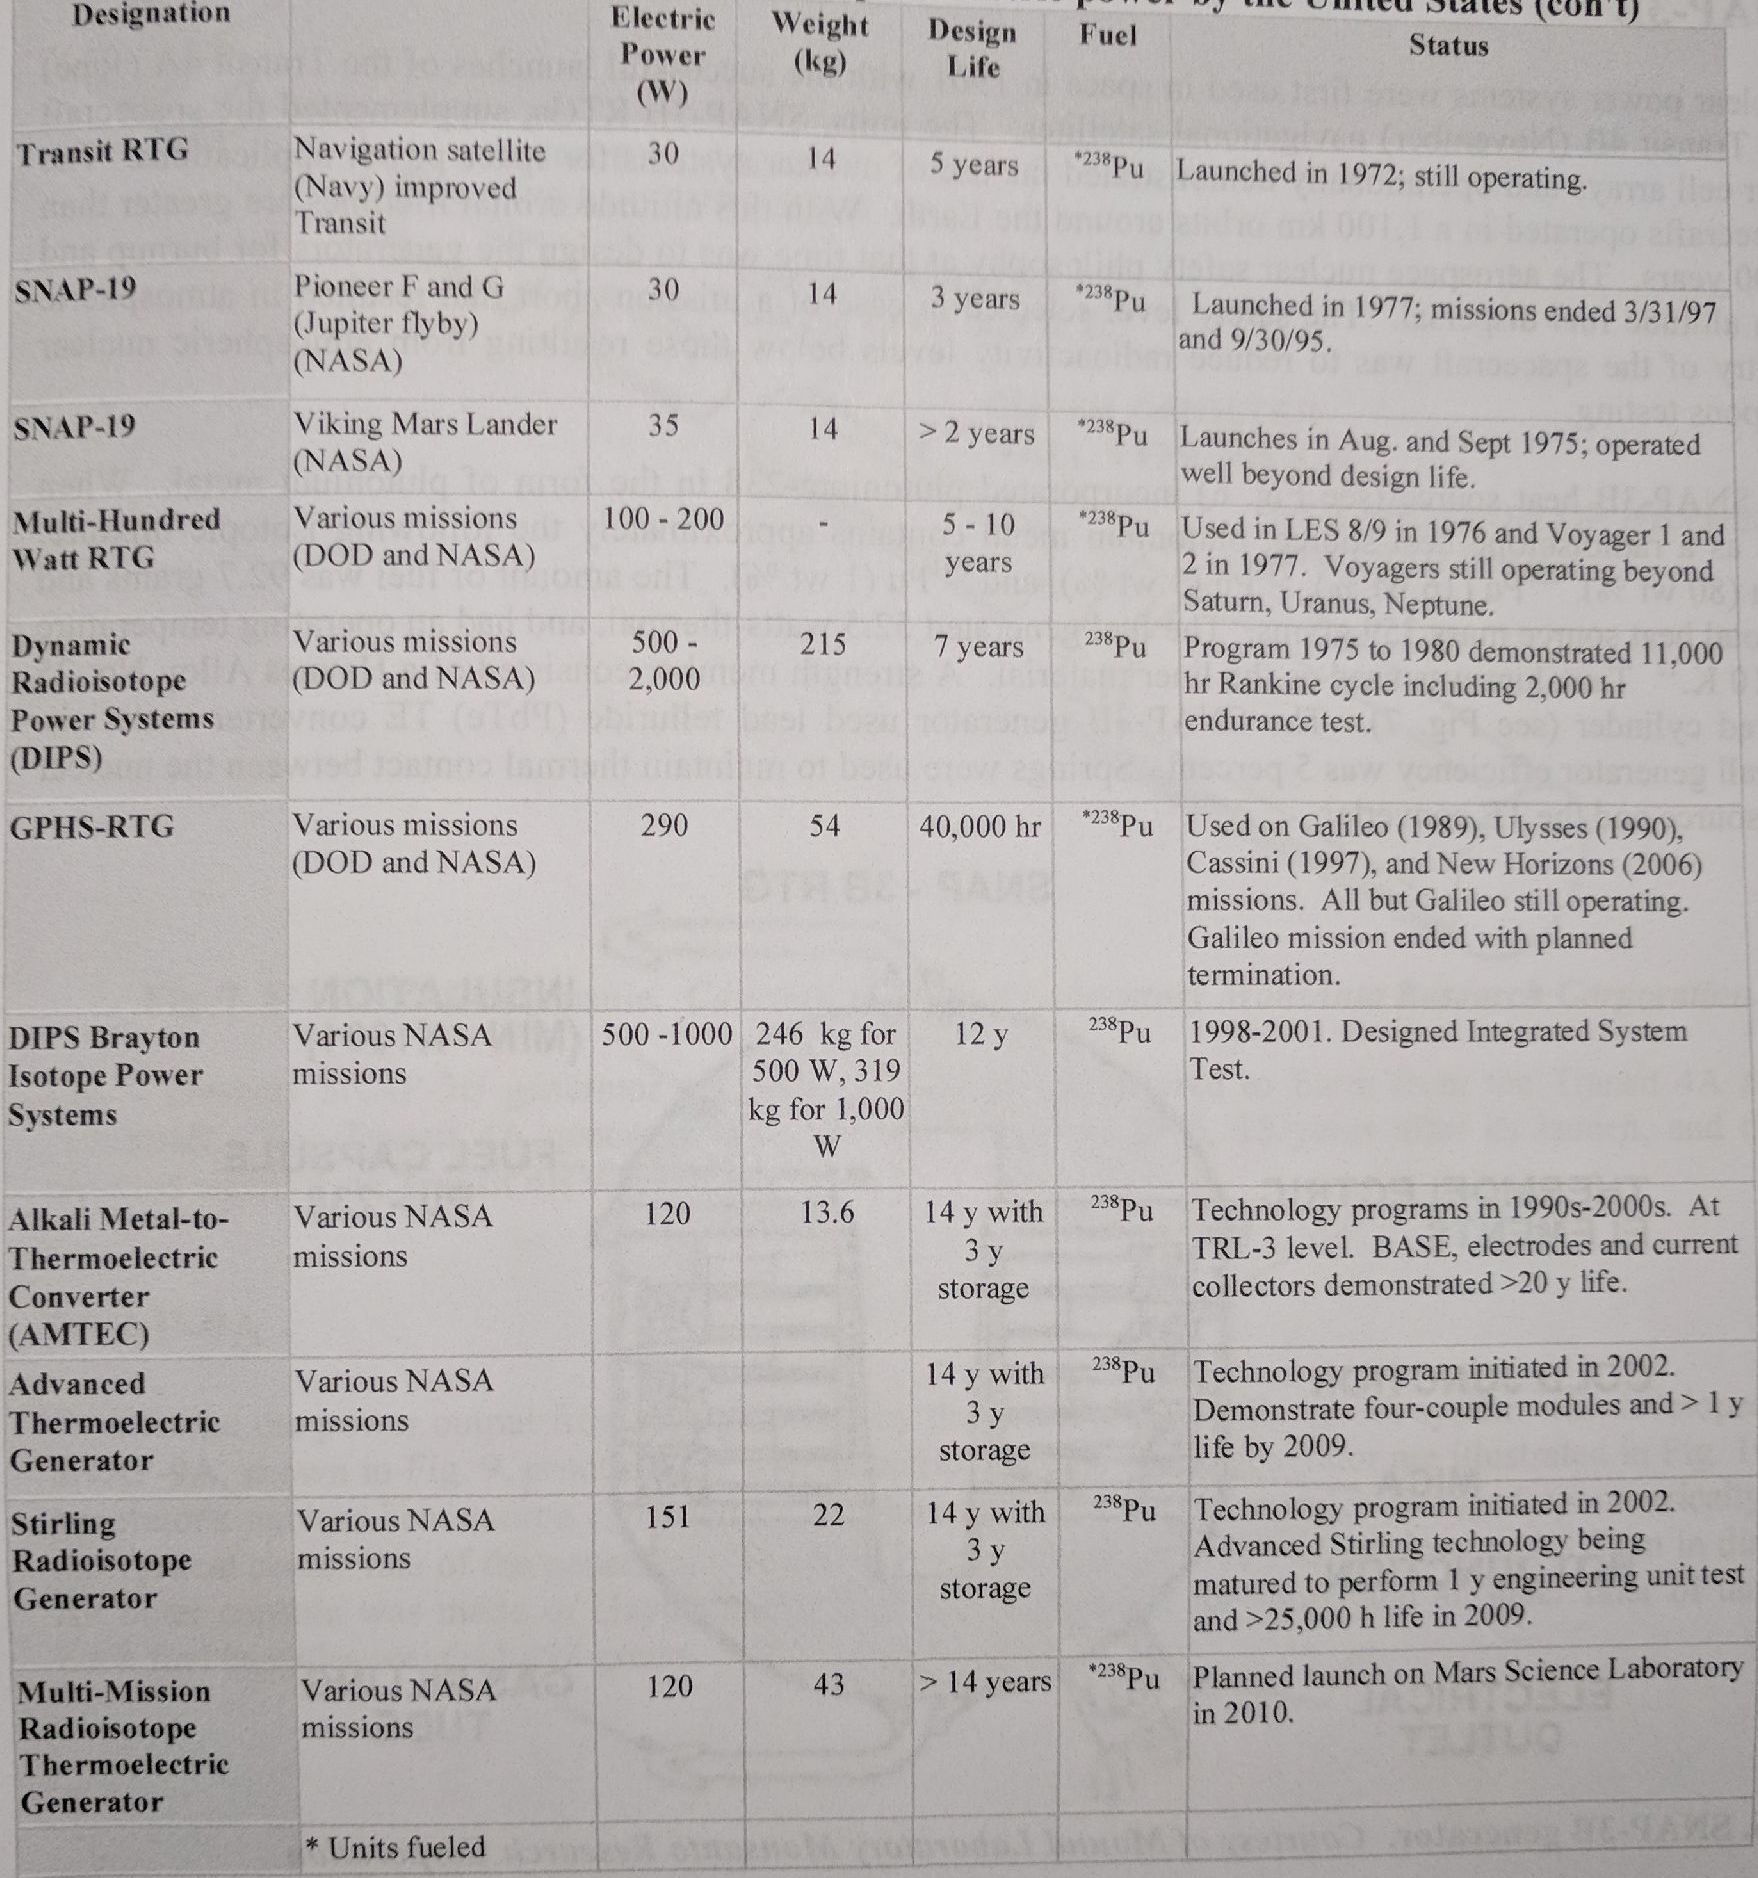
\includegraphics[height=0.55\textheight]{fig/table3}
	\caption[Radioisotope Generators Developed for Space Electric Power by the USA]{Radioisotope Generators Developed for Space Electric Power by the USA~\cite{buden2011spacebook1}}
	\label{table3}
\end{figure}

\begin{figure}[]
	\centering
	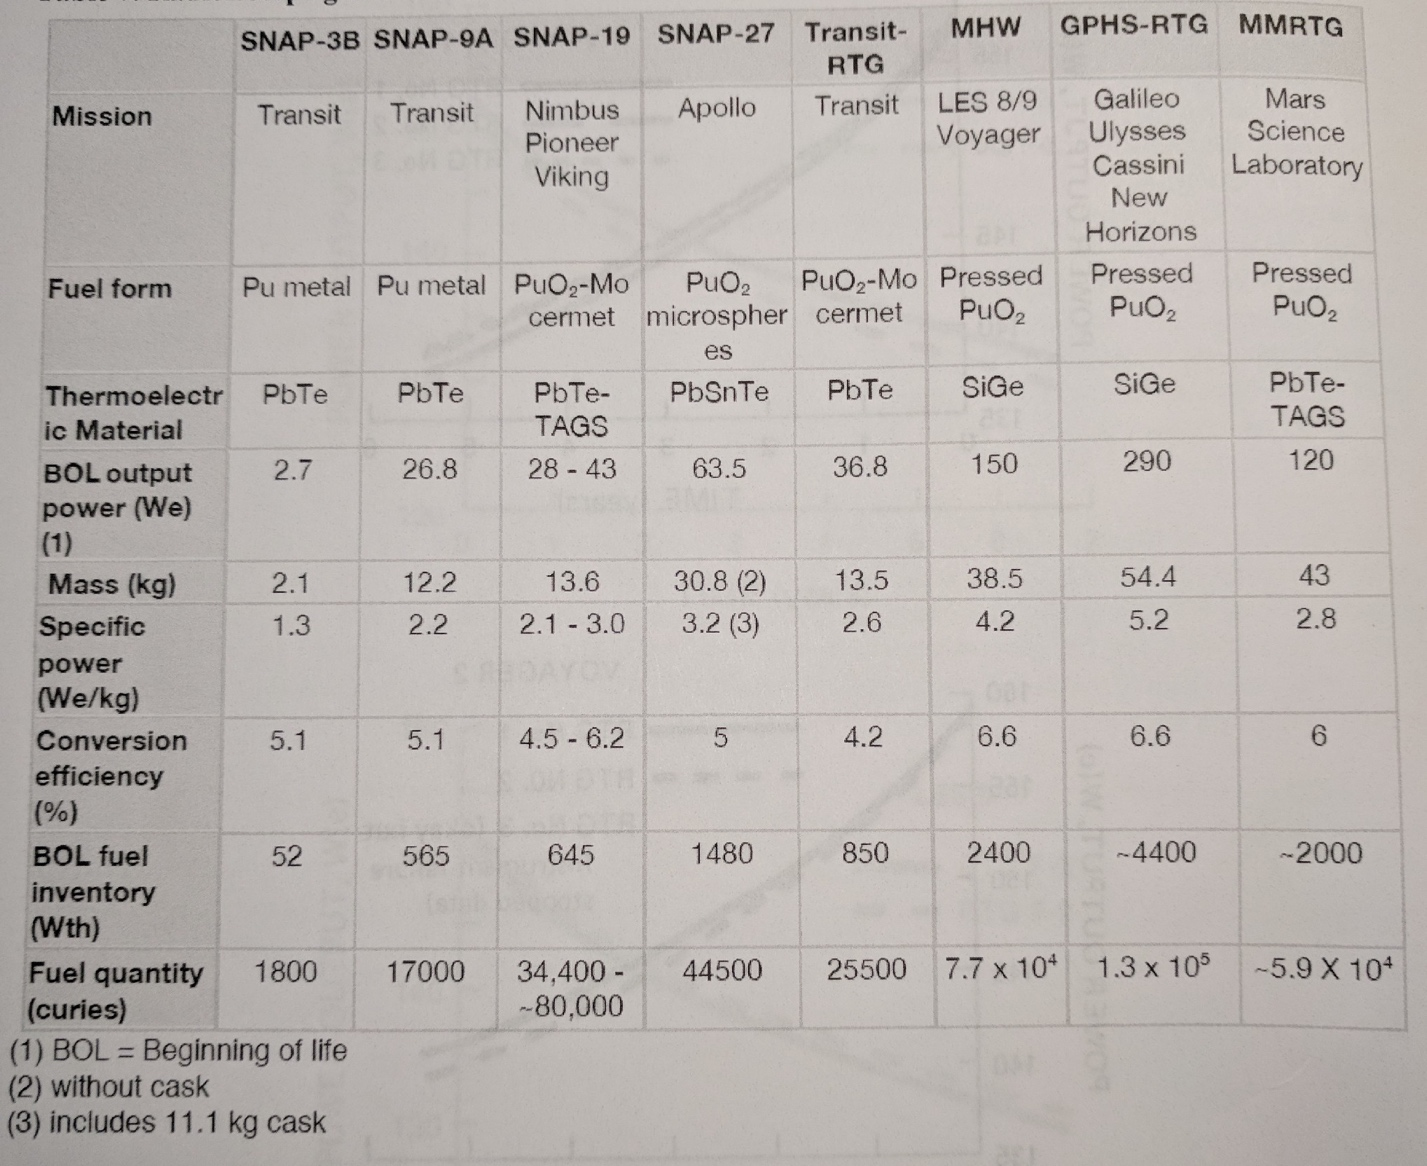
\includegraphics[height=0.35\textheight]{fig/table3bis}
	\caption[Radioisotope Generator Characteristics]{Radioisotope Generator Characteristics~\cite{buden2011spacebook1}}
	\label{table3bis}
\end{figure}


\subsection{Recent Radioisotope Generator Systems}

As space missions grew more advanced, more power was required to meet the electrical
needs of key onboard systems. Missions began to add extra generators to spacecraft, but this
meant that weight and volume were added. To curtail these drawbacks, modular power
systems were developed~\cite{bennett2006mission}. The first was the General Purpose Heat Source (GPHS) which replaced
the Multihundred Watt (MHW) generator systems~\cite{kelly1975mhw}. The GPHS has been proven through its use
on Galileo, Ulysses, Cassini, and most recently, New Horizons.

GPHS-RTG systems contain a stacked column of 18 modules in the fuel assembly and
572 silicon-germanium thermoelectric unicouples. Each of these modules produces around 245
W t and the system is capable of producing more than 300We. A TE converter surrounds the
GPHS heat source. The SiGe unicouples operate at a hot-side temperature of 1273K and a cold-
side reject temperature of 555K. They produce an electric efficiency of 6.6\%~\cite{lange1984tutorial}. Performance data
of the GPHS-RTG system is presented in Table~\ref{table4}.


\begin{figure}[]
	\centering
	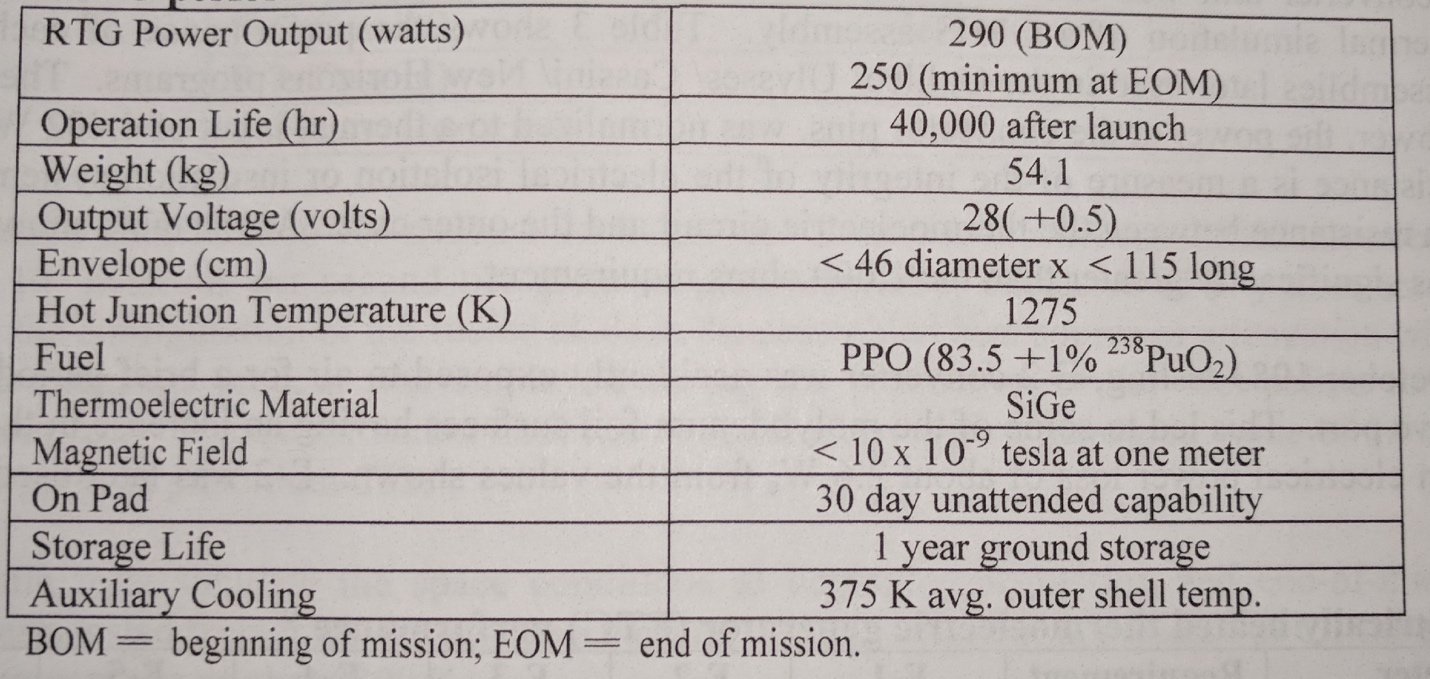
\includegraphics[height=0.35\textheight]{fig/table4}
	\caption[GPHS-RTG Performance]{GPHS-RTG Performance~\cite{buden2011spacebook1}}
	\label{table4}
\end{figure}

NASA is planning on using a Multi-Mission Radioisotope Thermoelectric Generator
(MMRTG) for the Mars Science Laboratory rover~\cite{von2006mmrtg}. An overview of the key system requirements
is presented in Table 5. The MMRTG is the latest generation of RTGs, and utilizes conversion
designs from the two Viking missions that landed on Mars. They are very similar to the SNAP-19
project. It combines a GPHS heat source that has had flight missions ranging from Galileo to
New Horizons, totaling more than nineteen years of operational success. The converters, using
lead telluride were used on SNAP-19 missions. The proven success of the GPHS power source and power conversion systems onboard Viking 1 and 2 show that MMRTG should be mission ready.


\begin{figure}[]
	\centering
	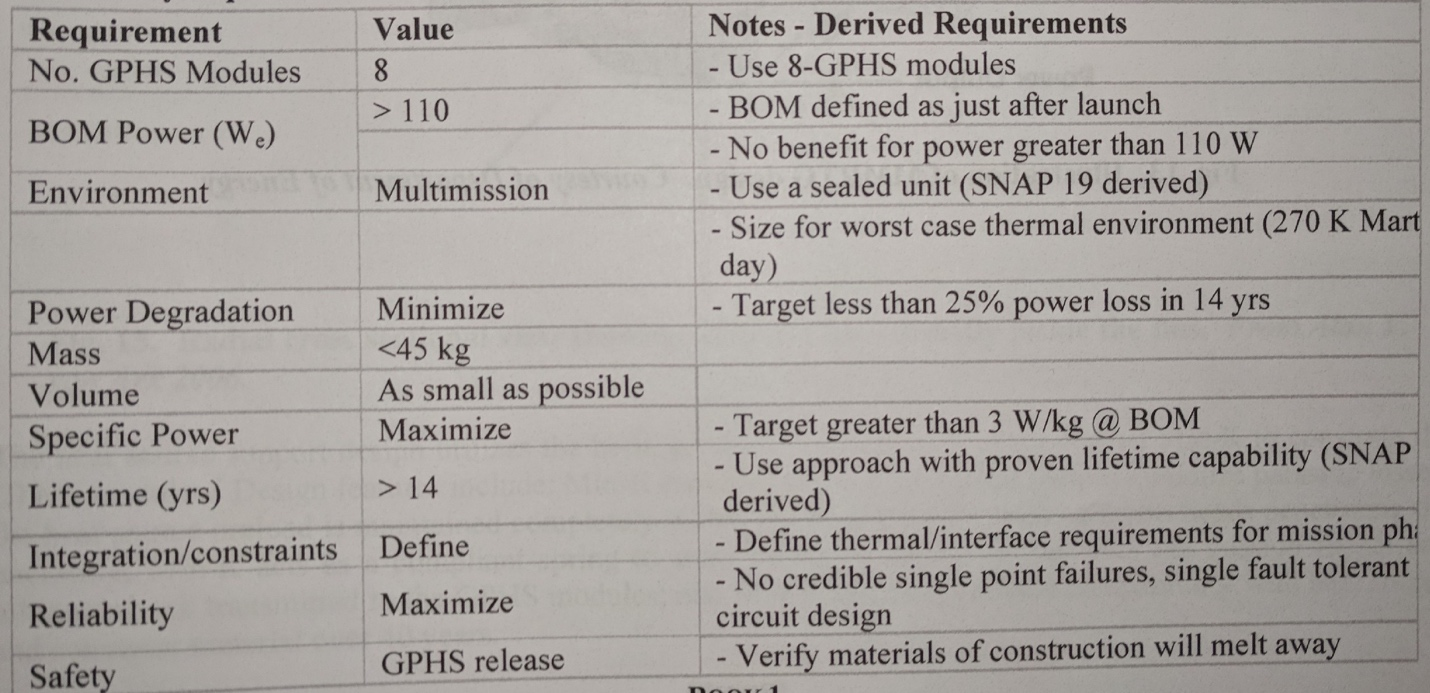
\includegraphics[height=0.35\textheight]{fig/table5}
	\caption[Requirements for MMRTG]{Requirements for MMRTG~\cite{buden2011spacebook1}}
	\label{table5}
\end{figure}

\subsection{Alternate Power Conversion Systems}

The expensive cost and low availability of plutonium-238 limits the use and creation of radioisotope power systems. Various programs have existed to develop higher efficiency conversion subsystems. Higher efficiencies and lighter weight conversion subsystems not only reduce the quantity of Pu-238 that is needed, but also reduce generator costs, and launch costs. Higher efficiencies also have the added benefit of making more power available to a spacecraft per unit volume or unit kg. The radioisotope heat sources are capable of coupling with dynamic thermal-to-electrical energy conversion systems, and are able to achieve efficiencies as high as three times that of traditional RTGs. Three systems, Brayton, Rankine, and Stirling types, have already been through development cycles~\cite{mason2007historical}.

\subsubsection{Brayton Isotope Power System (BIPS)}

The Brayton cycle follows several stages. A working fluid is kept in a gaseous state. Constant pressure heat addition is achieved from stage 1 to stage 2. Isentropic expansion occurs from stage 2 to stage 3 in the turbine to generate electricity. A portion of the output work at this stage goes to compressing the working fluid. Constant pressure at the heat rejection site occurs from stage 3 to stage 4. Isentropic compression occurs from stage 4 to stage 1. Figure~\ref{figure1} shows the process.

\begin{figure}[]
	\centering
	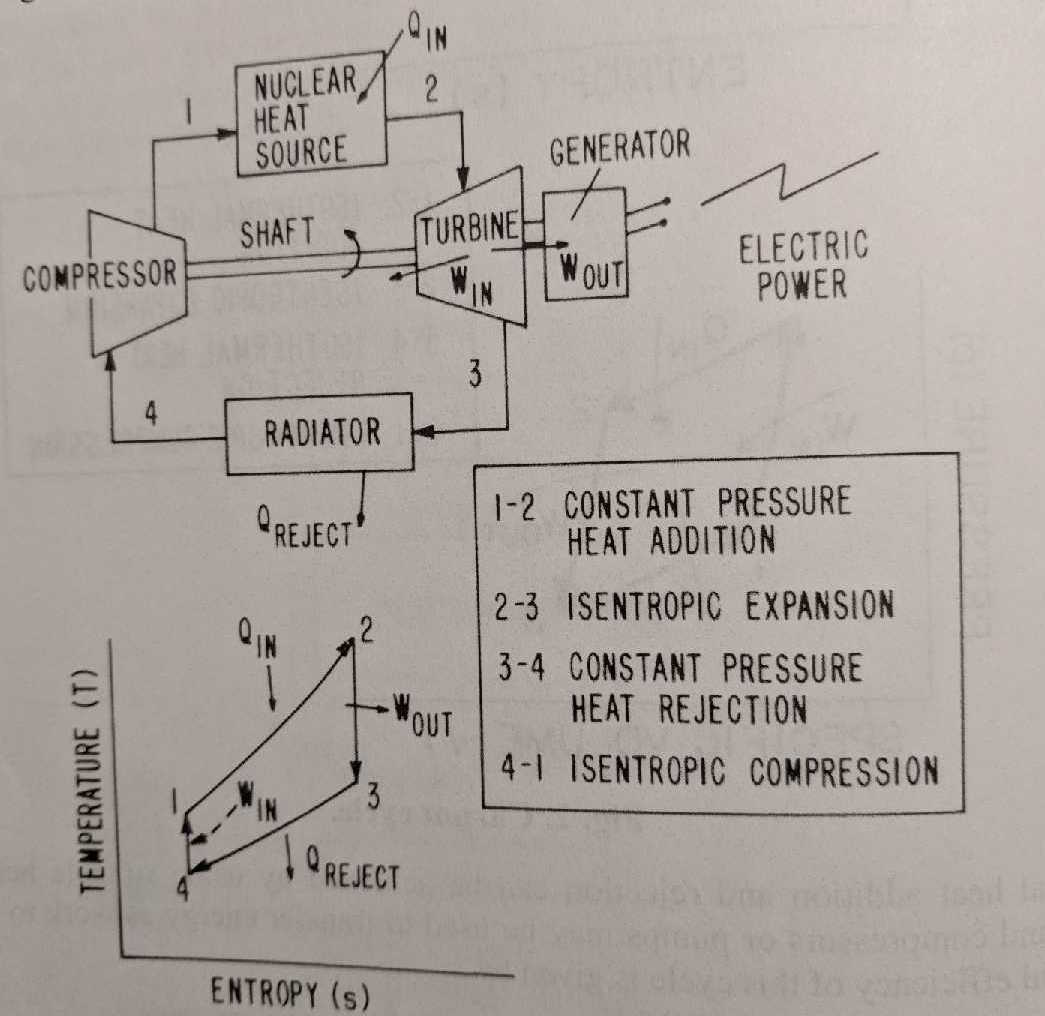
\includegraphics[height=0.45\textheight]{fig/figure1}
	\caption[Illustration of Brayton Cycle]{Illustration of Brayton Cycle~\cite{buden2011spacebook1}}
	\label{figure1}
\end{figure}


To increase the thermal efficiencies of the basic closed cycle, a regenerator can be employed. The regenerator uses the hot gases expelled from the turbine to preheat the working fluid as it exits the compressor. To further increase efficiencies, multistage compression with intercooling and multistage expansion with reheating may be employed. Ideally, the intercooler chills the gases to the initial inlet temperature before entering the next stage. The ideal regeneration system is presented in Figure~\ref{figure2}. 

\begin{figure}[]
	\centering
	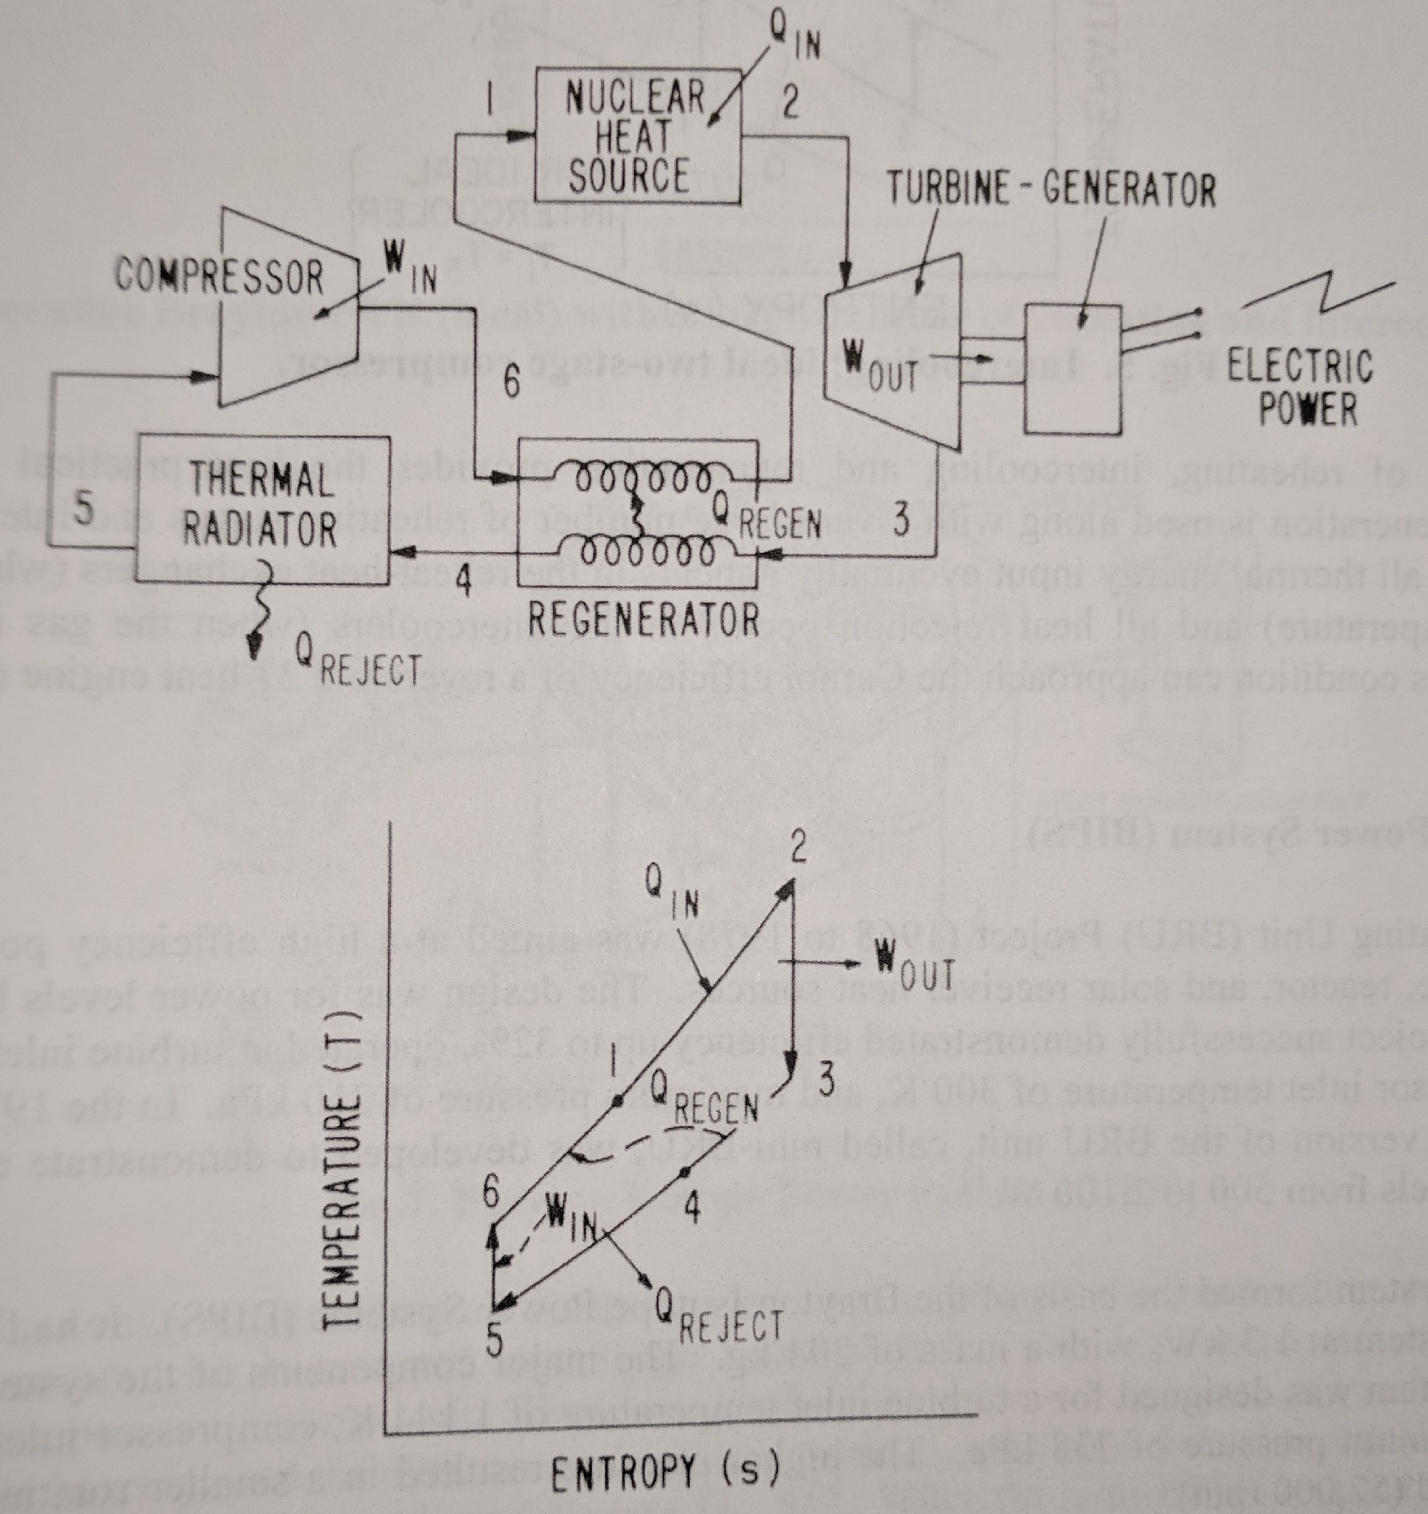
\includegraphics[height=0.45\textheight]{fig/figure2}
	\caption[Brayton Cycle with Regenerator]{Brayton Cycle with Regenerator~\cite{buden2011spacebook1}}
	\label{figure2}
\end{figure}


From 1968 to 1978, the Brayton Rotating Unit (BRU) was designed. It operated between 2.25 and 10.5 kWe and demonstrated efficiencies up to 32\%. The turbine operated at 1144K and the compressor temperature was 300K. from 1974 to 1978, the mini-BRU was developed. It was a smaller version of the conventional BRU, and demonstrated efficiencies of 30\% for power levels from 500-2100 Watts. 


	The mini-BRU laid the groundwork for the creation of the Brayton Isotope Power System (BIPS). BIPS demonstrated a system capable of 1.3kWe. It operated at a maximum pressure of 738 kPa, about double that of the BRU units. This higher pressure resulted in a smaller rotating assembly, with a higher shaft speed. The shaft was capable of spinning at more than 52,000 RPM. This shaft was the only rotating component in the whole assembly. BIPS accumulated 1000 hours of testing with no system problems. Brayton cycle components are presented in Table~\ref{table6}.

\begin{figure}[]
	\centering
	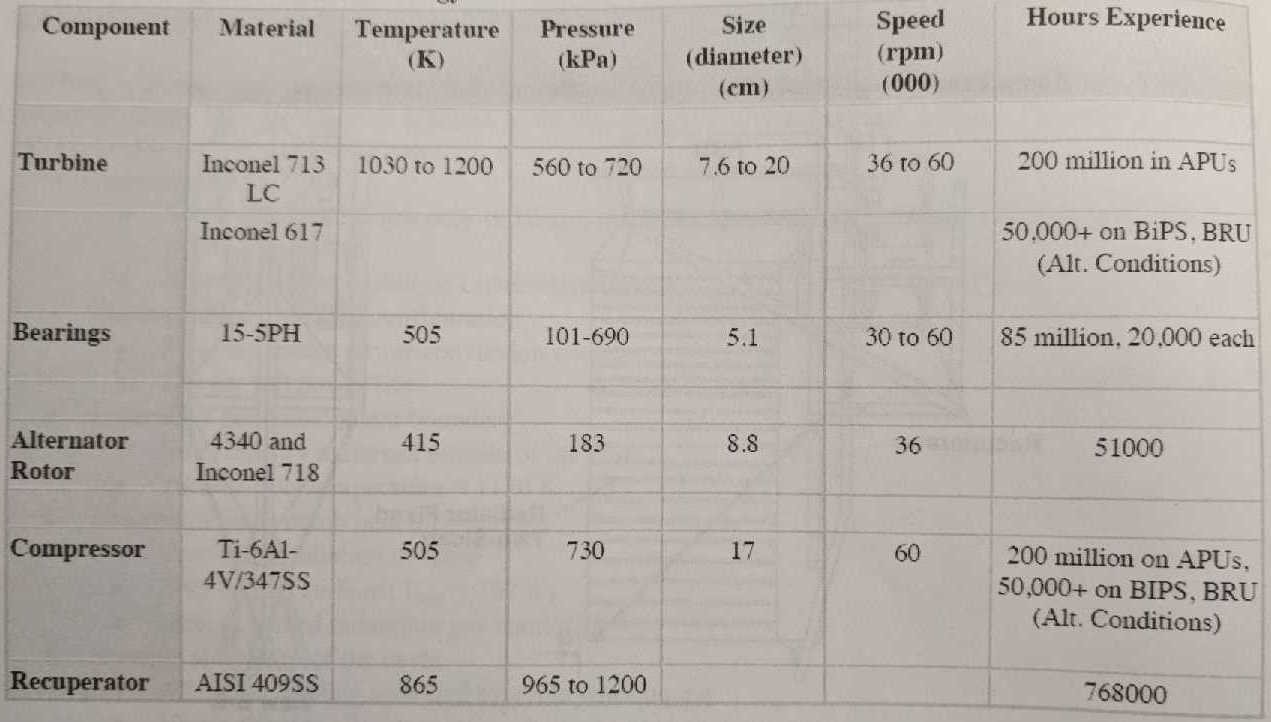
\includegraphics[height=0.45\textheight]{fig/table6}
	\caption[Power Conversion Technology for Brayton Cycle]{Power Conversion Technology for Brayton Cycle~\cite{buden2011spacebook1}}
	\label{table6}
\end{figure}


\subsubsection{Rankine Cycle Converters}

A Rankine cycle heat engine contains a heat source (the radioisotope fuel), a turbine-generator to convert heat to electricity, a heat radiator, and a pump to increase the working fluid pressure. The heat radiator causes the working fluid to experience a phase change, and rejects waste heat to space. A diagram of an ideal Rankine cycle heat engine is presented in Figure~\ref{figure3}.

\begin{figure}[]
	\centering
	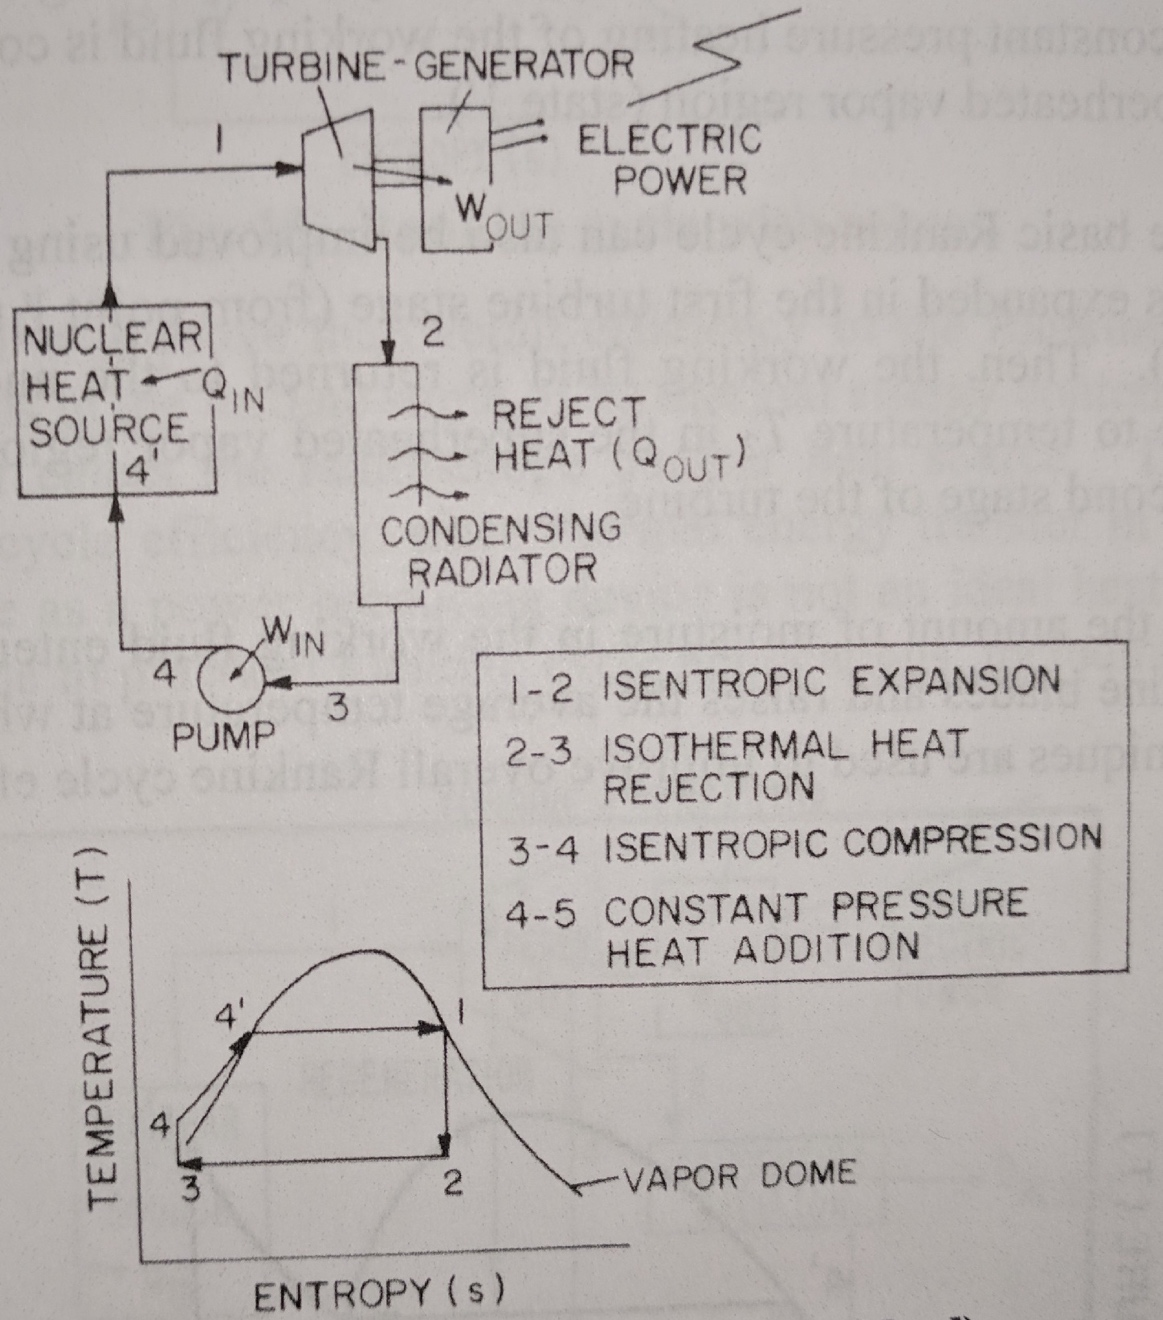
\includegraphics[height=0.45\textheight]{fig/figure3}
	\caption[Rankine Cycle]{Rankine Cycle~\cite{buden2011spacebook1}}
	\label{figure3}
\end{figure}


The Kilowatt Isotope Power System (KIPS) has been designed to use an organic working fluid Rankine cycle, and reached ground testing, though the program has now been inactive since 1980. Around 10\% of the working fluid flows through the regenerator. It spirals around tubes surrounding the heat source, where it becomes vapor at 630K. The vapor passes through the turbine to generate electricity. The system is capable of efficiencies of 18.1\%. A table of a Dynamic Isotope Power System (DIPS) is presented in Table~\ref{table7}~\cite{pearson1988dynamic}.

\begin{figure}[]
	\centering
	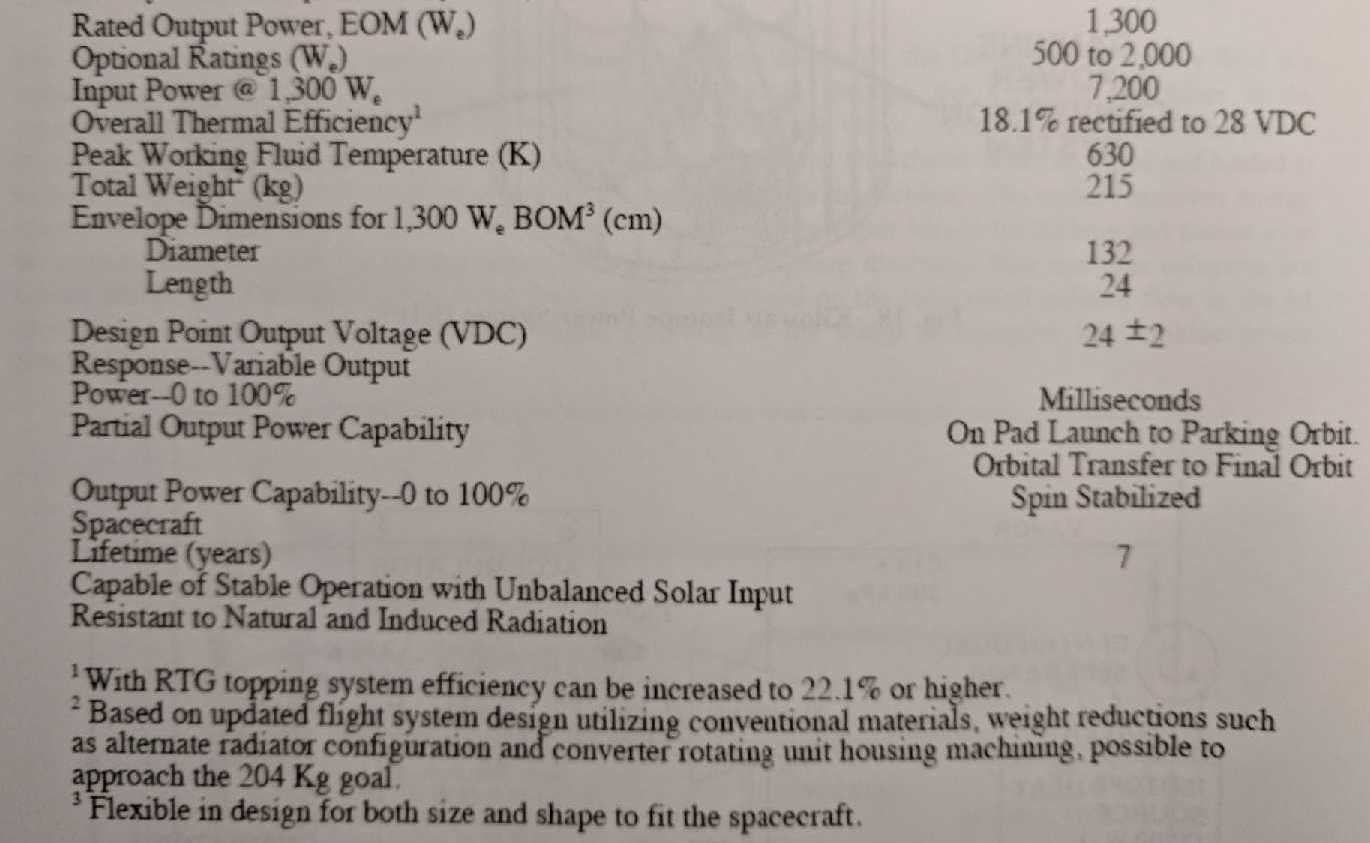
\includegraphics[height=0.45\textheight]{fig/table7}
	\caption[Dynamic Isotope Power System Overview]{Dynamic Isotope Power System Overview~\cite{buden2011spacebook1}}
	\label{table7}
\end{figure}

\subsubsection{Stirling Cycle Converters}

Stirling engines were first designed in the early 19th century. A regenerator is incorporated to store heat, then reversibly recover it. Working fluid transfers heat and drops in temperature. Then, as it passes back through the regenerator, it regains the heat that was stored there. A free piston Stirling engine (FPSE) has been examined for space applications~\cite{goldwater1977demonstration}. 


	An FPSE consists of three major components, a power piston, a displacer piston, and a sealed cylinder. The two pistons are the only two moving parts in the system. Figure~\ref{figure4} shows a simple schematic of the system.

\begin{figure}[]
	\centering
	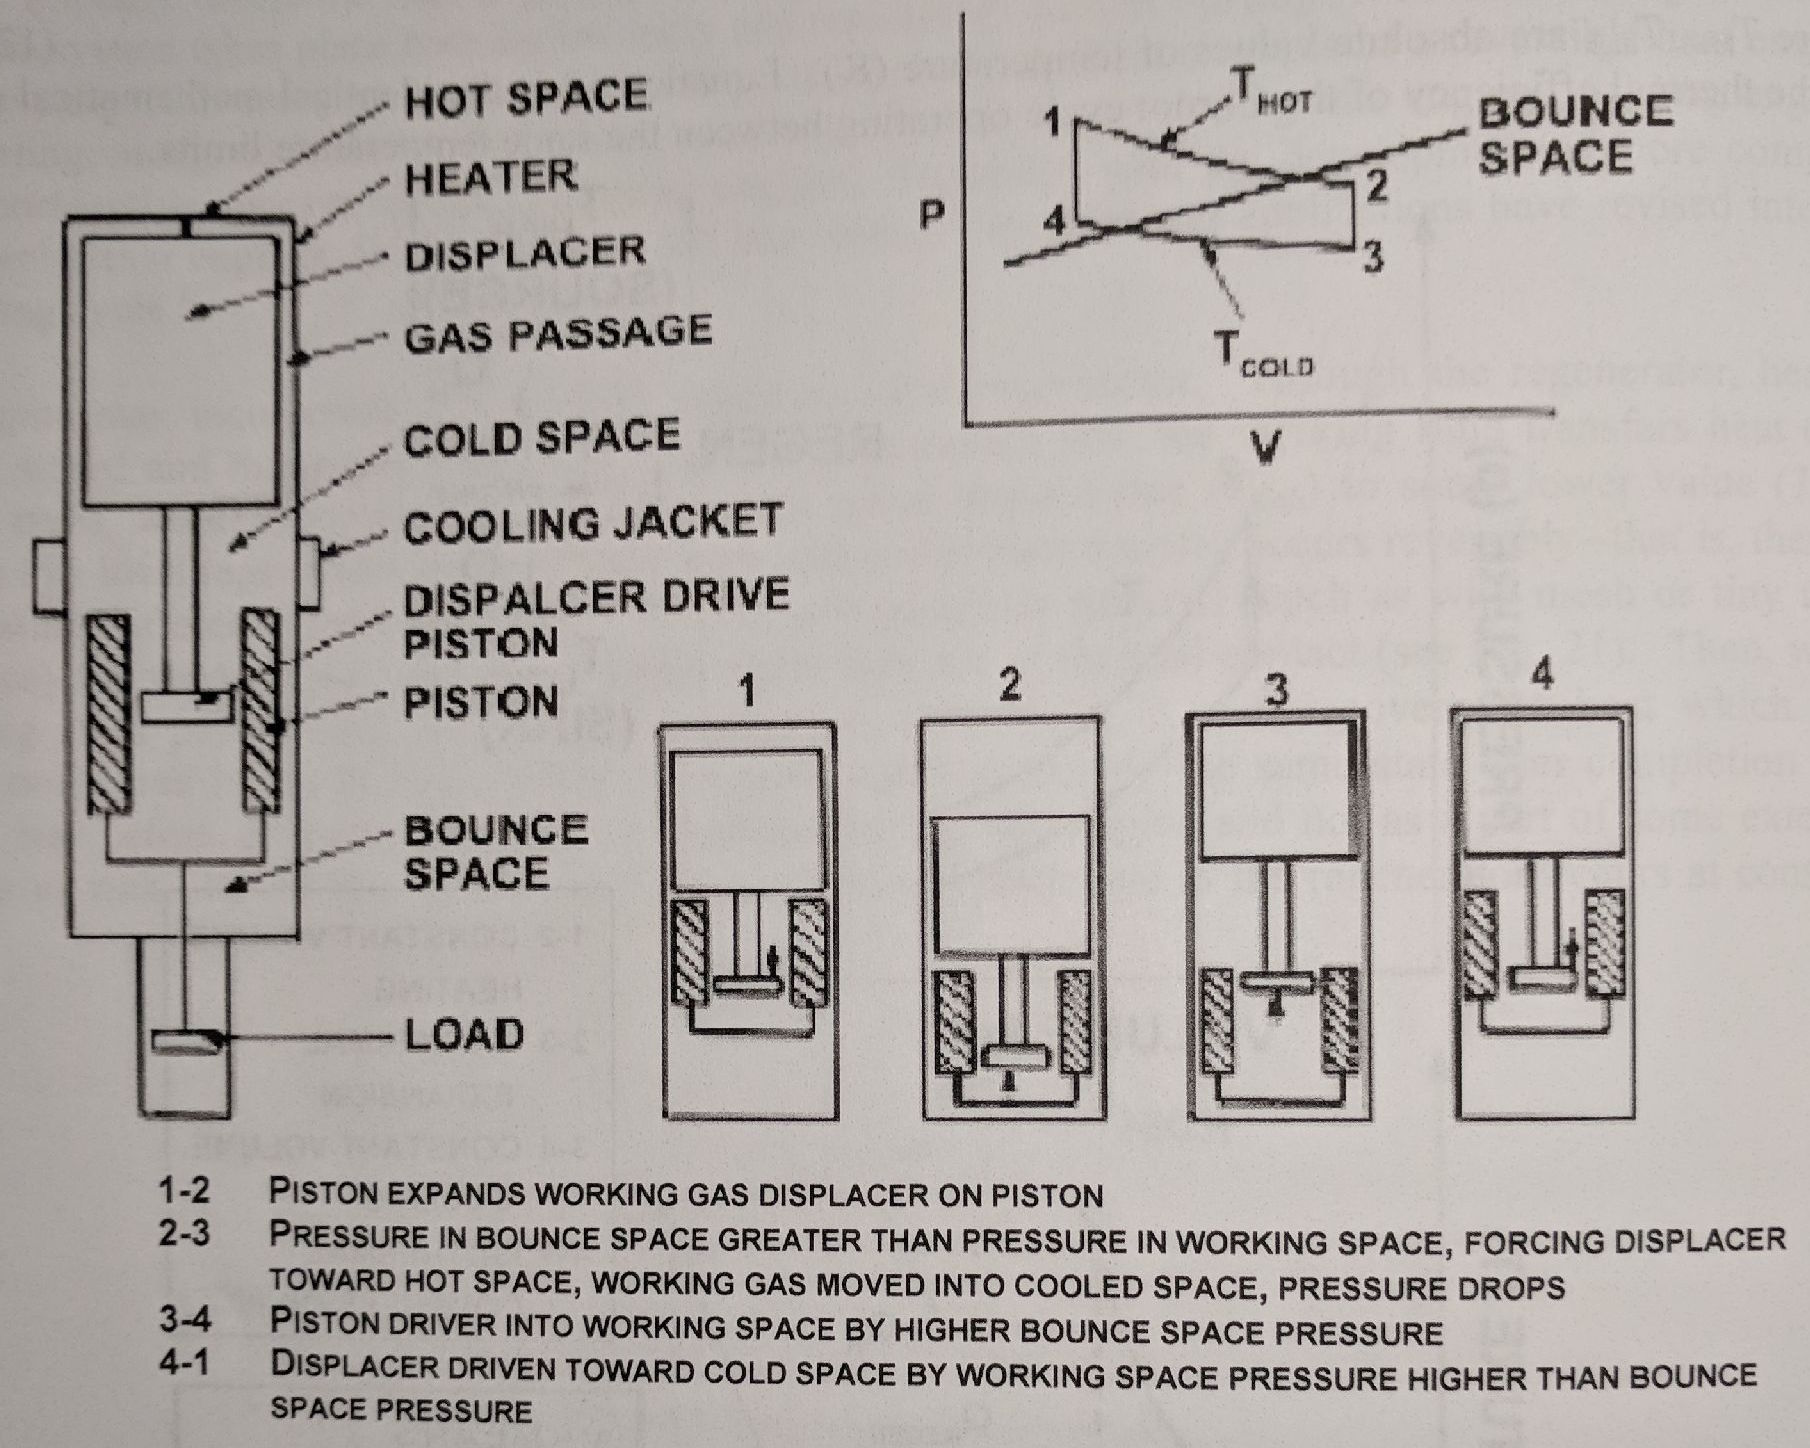
\includegraphics[height=0.45\textheight]{fig/figure4}
	\caption[Stirling Cycle]{Stirling Cycle~\cite{buden2011spacebook1}}
	\label{figure4}
\end{figure}


The Advanced Stirling Radioisotope Generator (ASRG) uses two Stirling engines for power production~\cite{wood2006advanced}. They are coaxially aligned to minimize any vibrations from operation. ASRG's are designed to produce 151 We and can operate for 14 years or more. They are capable of nearly 40\% efficiencies. 

\subsubsection{Advanced Thermoelectric Converters}

Current TE converters achieve efficiencies of only 6\%. New advancements in the technology aim to increase performance of We/kg by 57\%. They aim to improve efficiencies by 8-10\% over traditional GPHS-RTGs and MMRTGs~\cite{mondt2002advanced}.

\subsubsection{Alkali Metal Thermal-To-Electric Converters}

Alkali Metal Thermal-To-Electric Converters (AMTEC) use thermally regenerative electrochemical devices to convert the heat generated directly to electricity~\cite{spence2003development}. They are still under development, but could prove to be advantageous as there are no moving parts. A sodium concentration cell using beta-alumina solid electrolytes (BASE) as a separator between the high and low pressure regions is being considered. AMTEC is forecasted to provide 20We/kg with 15-20\% conversion efficiency. Several problems still exist for the design that have prevented its implementation, including problems developing a BASE to metal ceramic seal, and problems developing an electrical feed-through fabrication process. 










\section{Conclusions}

The limitations for our mission are to have a bimodal nuclear thermal rocket and to use low enriched uranium. Based on our preliminary research, our team has decided to proceed basing our rocket on the heatpipe design described earlier. The main advantages to the heatpipe system are reliability, compactness, and longevity, as fuel burnup limits will not be reached for several decades. Since the Oort
cloud is, at its closest, 5,000 AU away, longevity is one of the most important factors for our rocket.

Potential problems with the heatpipe system are the fuel and low power. All the fuels tested have been highly enriched uranium, usually around 95+\%. The most promising heatpipe system has an output of 100 kWe, which may not be enough power. However, due to their versatility and longevity, they seem to be the best option to meet our mission goals and limitations.


\section*{Acronyms}
\addcontentsline{toc}{section}{Acronyms}

\begin{tabular}{ l  l }
    $SCoRE$       &Sectored Compact Space Reactor\\
    $HOMER$         &Heatpipe-Operated Mars Exploration Reactor\\
    $SAFE$         &Safe Affordable Fission Engine\\
    $UN$         & Uranium nitride\\
    $UO2$         & Uranium dioxide\\
    $SS$           & Stainless Steel\\
    $S^4$         & Submersion-Subcritical Safe Space reactor\\
    $HEU$         & High Enriched Uranium\\
    $LEU$         & Low Enriched Uranium\\
    $NTP$  & Nuclear Thermal Propulsion\\
    $RTG$  & Radioisotope thermoelectric generators\\
    $SNAP$  & Systems for Nuclear Auxiliary Power\\
    $SER$   & SNAP Experimental Reactor\\
    $GPHS$  & General Purpose Heat Source\\
    $MHW$ & Multihundred Watt\\
    $MMRTG$  & Multi-Mission Radioisotope Thermoelectric Generator\\
 \end{tabular}


\clearpage
% Bibliography
% ---------------------------------------------------------------------------------
\bibliographystyle{apacite}
\bibliography{pfbn}
% ---------------------------------------------------------------------------------


\end{document}


